\documentclass[12pt]{article}

\author{Matthew D. Cocci}
\title{Asset Pricing}
\date{\today}

%% Formatting & Spacing %%%%%%%%%%%%%%%%%%%%%%%%%%%%%%%%%%%%

%\usepackage[top=1in, bottom=1in, left=1in, right=1in]{geometry} % most detailed page formatting control
\usepackage{fullpage} % Simpler than using the geometry package; std effect
\usepackage{setspace}
%\onehalfspacing
\usepackage{microtype}

%% Formatting %%%%%%%%%%%%%%%%%%%%%%%%%%%%%%%%%%%%%%%%%%%%%

%\usepackage[margin=1in]{geometry}
    %   Adjust the margins with geometry package
%\usepackage{pdflscape}
    %   Allows landscape pages
%\usepackage{layout}
    %   Allows plotting of picture of formatting
\usepackage{multicol}
\setlength{\columnsep}{1cm}



%% Header %%%%%%%%%%%%%%%%%%%%%%%%%%%%%%%%%%%%%%%%%%%%%%%%%

%\usepackage{fancyhdr}
%\pagestyle{fancy}
%\lhead{}
%\rhead{}
%\chead{}
%\setlength{\headheight}{15.2pt}
    %   Make the header bigger to avoid overlap

%\fancyhf{}
    %   Erase header settings

%\renewcommand{\headrulewidth}{0.3pt}
    %   Width of the line

%\setlength{\headsep}{0.2in}
    %   Distance from line to text


%% Mathematics Related %%%%%%%%%%%%%%%%%%%%%%%%%%%%%%%%%%%

\usepackage{amsmath}
\usepackage{amssymb}
\usepackage{amsfonts}
\usepackage{mathrsfs}
\usepackage{amsthm} %allows for labeling of theorems
\theoremstyle{plain}
\newtheorem{thm}{Theorem}[section]
\newtheorem{lem}[thm]{Lemma}
\newtheorem{prop}[thm]{Proposition}
\newtheorem{cor}[thm]{Corollary}
\newtheorem{ax}[thm]{Axiom}

\theoremstyle{definition}
\newtheorem{defn}[thm]{Definition}
\newtheorem{ex}[thm]{Example}
\newtheorem{assump}[thm]{Assumption}

\theoremstyle{remark}
\newtheorem*{rmk}{Remark}
\newtheorem*{note}{Note}

% Below supports left-right alignment in matrices so the negative
% signs don't look bad
\makeatletter
\renewcommand*\env@matrix[1][c]{\hskip -\arraycolsep
  \let\@ifnextchar\new@ifnextchar
  \array{*\c@MaxMatrixCols #1}}
\makeatother


%% Font Choices %%%%%%%%%%%%%%%%%%%%%%%%%%%%%%%%%%%%%%%%%

\usepackage[T1]{fontenc}
\usepackage{lmodern}
\usepackage[utf8]{inputenc}
%\usepackage{blindtext}
\usepackage{courier}


%% Figures %%%%%%%%%%%%%%%%%%%%%%%%%%%%%%%%%%%%%%%%%%%%%%

\usepackage{tikz}
%\usepackage{tikz-3dplot}
\usetikzlibrary{decorations.pathreplacing}
\usetikzlibrary{patterns}
\usepackage{graphicx}
\usepackage{subfigure}
    %   For plotting multiple figures at once
%\graphicspath{ {Directory/} }
    %   Set a directory for where to look for figures

%\pgfdeclarepatternformonly[\LineSpace]{my north east lines}{\pgfqpoint{-1pt}{-1pt}}{\pgfqpoint{\LineSpace}{\LineSpace}}{\pgfqpoint{\LineSpace}{\LineSpace}}%
%{
    %\pgfsetlinewidth{0.4pt}
    %\pgfpathmoveto{\pgfqpoint{0pt}{0pt}}
    %\pgfpathlineto{\pgfqpoint{\LineSpace + 0.1pt}{\LineSpace + 0.1pt}}
    %\pgfusepath{stroke}
%}

%\pgfdeclarepatternformonly[\LineSpace]{my north west lines}{\pgfqpoint{-1pt}{-1pt}}{\pgfqpoint{\LineSpace}{\LineSpace}}{\pgfqpoint{\LineSpace}{\LineSpace}}%
%{
    %\pgfsetlinewidth{0.4pt}
    %\pgfpathmoveto{\pgfqpoint{0pt}{\LineSpace}}
    %\pgfpathlineto{\pgfqpoint{\LineSpace + 0.1pt}{-0.1pt}}
    %\pgfusepath{stroke}
%}

%\newdimen\LineSpace
%\tikzset{
    %line space/.code={\LineSpace=#1},
    %line space=3pt
%}


%% Hyperlinks %%%%%%%%%%%%%%%%%%%%%%%%%%%%%%%%%%%%%%%%%%%%
\usepackage{hyperref}
\hypersetup{%
    colorlinks,
        %   This colors the links themselves, not boxes
    citecolor=black,
        %   Everything here and below changes link colors
    filecolor=black,
    linkcolor=black,
    urlcolor=black
}

%% Colors %%%%%%%%%%%%%%%%%%%%%%%%%%%%%%%%%%%%%%%%%%%%%%%

\usepackage{color}
\definecolor{codegreen}{RGB}{28,172,0}
\definecolor{codelilas}{RGB}{170,55,241}

% David4 color scheme
\definecolor{d4blue}{RGB}{100,191,255}
\definecolor{d4gray}{RGB}{175,175,175}
\definecolor{d4black}{RGB}{85,85,85}
\definecolor{d4orange}{RGB}{255,150,100}


%% Including Code %%%%%%%%%%%%%%%%%%%%%%%%%%%%%%%%%%%%%%%

\usepackage{verbatim}
    %   For including verbatim code from files, no colors
\usepackage{listings}
    %   For including code snippets written directly in this doc

\lstdefinestyle{bash}{%
  language=bash,%
  basicstyle=\footnotesize\ttfamily,%
  showstringspaces=false,%
  commentstyle=\color{gray},%
  keywordstyle=\color{blue},%
  xleftmargin=0.25in,%
  xrightmargin=0.25in
}

\lstdefinestyle{matlab}{%
  language=Matlab,%
  basicstyle=\footnotesize\ttfamily,%
  breaklines=true,%
  morekeywords={matlab2tikz},%
  keywordstyle=\color{blue},%
  morekeywords=[2]{1}, keywordstyle=[2]{\color{black}},%
  identifierstyle=\color{black},%
  stringstyle=\color{codelilas},%
  commentstyle=\color{codegreen},%
  showstringspaces=false,%
    %   Without this there will be a symbol in
    %   the places where there is a space
  numbers=left,%
  numberstyle={\tiny \color{black}},%
    %   Size of the numbers
  numbersep=9pt,%
    %   Defines how far the numbers are from the text
  emph=[1]{for,end,break,switch,case},emphstyle=[1]\color{red},%
    %   Some words to emphasise
}

\newcommand{\matlabcode}[1]{%
    \lstset{style=matlab}%
    \lstinputlisting{#1}
}
    %   For including Matlab code from .m file with colors,
    %   line numbering, etc.

%% Bibliographies %%%%%%%%%%%%%%%%%%%%%%%%%%%%%%%%%%%%

\usepackage{natbib}
    %---For bibliographies
%\setlength{\bibsep}{3pt} % Set how far apart bibentries are


%% Misc %%%%%%%%%%%%%%%%%%%%%%%%%%%%%%%%%%%%%%%%%%%%%%

\usepackage{enumitem}
    %   Has to do with enumeration
\usepackage{appendix}
%\usepackage{natbib}
    %   For bibliographies
\usepackage{pdfpages}
    %   For including whole pdf pages as a page in doc


%% User Defined %%%%%%%%%%%%%%%%%%%%%%%%%%%%%%%%%%%%%%%%%%

%\newcommand{\nameofcmd}{Text to display}
\newcommand*{\Chi}{\mbox{\large$\chi$}} %big chi
    %   Bigger Chi

% In math mode, Use this instead of \munderbar, since that changes the
% font from math to regular
\makeatletter
\def\munderbar#1{\underline{\sbox\tw@{$#1$}\dp\tw@\z@\box\tw@}}
\makeatother

% Misc Math
\newcommand{\ra}{\rightarrow}
\newcommand{\diag}{\text{diag}}
\newcommand{\proj}{\operatorname{proj}}
\newcommand{\ch}{\text{ch}}
\newcommand{\dom}{\text{dom}}
\newcommand{\one}[1]{\mathbf{1}_{#1}}


% Command to generate new math commands:
% - Suppose you want to refer to \boldsymbol{x} as just \bsx, where 'x'
%   is any letter. This commands lets you generate \bsa, \bsb, etc.
%   without copy pasting \newcommand{\bsa}{\boldsymbol{a}} for each
%   letter individually. Instead, just include
%
%     \generate{bs}{\boldsymbol}{a,...,z}
%
% - Uses pgffor package to loop
% - Example with optional argument. Will generate \bshatx to represent
%   \boldsymbol{\hat{x}} for all letters x
%
%     \generate[\hat]{bshat}{\boldsymbol}{a,...,z}

\newcommand{\generate}[4][]{%
  % Takes 3 arguments (maybe four):
  % - 1   wrapcmd (optional, defaults to nothing)
  % - 2   newname
  % - 3   mathmacro
  % - 4   Names to loop over
  %
  % Will produce
  %
  %   \newcommand{\newnameX}{mathmacro{wrapcmd{X}}}
  %
  % for each X in argument 4

  \foreach \x in {#4}{%
    \expandafter\xdef\csname%
      #2\x%
    \endcsname%
    {\noexpand\ensuremath{\noexpand#3{\noexpand#1{\x}}}}
  }
}

% MATHSCR: Gen \sX to stand for \mathscr{X} for all upper case letters
\generate{s}{\mathscr}{A,...,Z}


% BOLDSYMBOL: Generate \bsX to stand for \boldsymbol{X}, all upper and
% lower case.
%
% Letters and greek letters
\generate{bs}{\boldsymbol}{a,...,z}
\generate{bs}{\boldsymbol}{A,...,Z}
\newcommand{\bseta}{\boldsymbol{\eta}}
\newcommand{\bstheta}{\boldsymbol{\theta}}
\newcommand{\bsTheta}{\boldsymbol{\Theta}}
\newcommand{\bsmu}{\boldsymbol{\mu}}
\newcommand{\bsSigma}{\boldsymbol{\Sigma}}
\newcommand{\bssigma}{\boldsymbol{\sigma}}
\newcommand{\bsvarepsilon}{\boldsymbol{\varepsilon}}
\newcommand{\bsalpha}{\boldsymbol{\alpha}}
\newcommand{\bsbeta}{\boldsymbol{\beta}}
\newcommand{\bsPi}{\boldsymbol{\Pi}}
\newcommand{\bsgamma}{\boldsymbol{\gamma}}
\newcommand{\bsGamma}{\boldsymbol{\Gamma}}
\newcommand{\bslambda}{\boldsymbol{\lambda}}
\newcommand{\bsLambda}{\boldsymbol{\Lambda}}
\newcommand{\bshatLambda}{\boldsymbol{\hat{\Lambda}}}
\newcommand{\bshatG}{\boldsymbol{\hat{G}}}
\newcommand{\bsdelta}{\boldsymbol{\delta}}
\newcommand{\bsOmega}{\boldsymbol{\Omega}}
\newcommand{\bsPsi}{\boldsymbol{\Psi}}
\newcommand{\bspsi}{\boldsymbol{\psi}}
\newcommand{\bsPhi}{\boldsymbol{\Phi}}
\newcommand{\bsphi}{\boldsymbol{\phi}}

% Special cases like \bshatb for \boldsymbol{\hat{b}}
\generate[\hat]{bshat}{\boldsymbol}{a,b,y,x,X,V,S,W,A,B,P}
\newcommand{\bshatbeta}{\boldsymbol{\hat{\beta}}}
\newcommand{\bshatmu}{\boldsymbol{\hat{\mu}}}
\newcommand{\bshattheta}{\boldsymbol{\hat{\theta}}}
\newcommand{\bsbartheta}{\boldsymbol{\bar{\theta}}}
\newcommand{\bshatSigma}{\boldsymbol{\hat{\Sigma}}}
\newcommand{\bstildebeta}{\boldsymbol{\tilde{\beta}}}
\newcommand{\bstildetheta}{\boldsymbol{\tilde{\theta}}}
\newcommand{\bstildePsi}{\boldsymbol{\tilde{\Psi}}}
\newcommand{\bsbarbeta}{\boldsymbol{\overline{\beta}}}
\newcommand{\bshatOmega}{\boldsymbol{\hat{\Omega}}}
\newcommand{\bsbarg}{\boldsymbol{\overline{g}}}
\newcommand{\bstildey}{\boldsymbol{\tilde{y}}}
\newcommand{\bstildeX}{\boldsymbol{\tilde{X}}}
\newcommand{\bstildevarepsilon}{\boldsymbol{\tilde{\varepsilon}}}
\newcommand{\bstildes}{\boldsymbol{\tilde{s}}}
\newcommand{\bstildeT}{\boldsymbol{\tilde{T}}}
\newcommand{\bstildeC}{\boldsymbol{\tilde{C}}}

% Zero vector as \bso
\renewcommand{\bso}{\boldsymbol{0}}

% Transposes of all the boldsymbol shit
\newcommand{\bsbp}{\boldsymbol{b'}}
\newcommand{\bshatbp}{\boldsymbol{\hat{b'}}}
\newcommand{\bsdp}{\boldsymbol{d'}}
\newcommand{\bsgp}{\boldsymbol{g'}}
\newcommand{\bsGp}{\boldsymbol{G'}}
\newcommand{\bshp}{\boldsymbol{h'}}
\newcommand{\bsSp}{\boldsymbol{S'}}
\newcommand{\bsup}{\boldsymbol{u'}}
\newcommand{\bsxp}{\boldsymbol{x'}}
\newcommand{\bsyp}{\boldsymbol{y'}}
\newcommand{\bsthetap}{\boldsymbol{\theta'}}
\newcommand{\bsmup}{\boldsymbol{\mu'}}
\newcommand{\bsSigmap}{\boldsymbol{\Sigma'}}
\newcommand{\bshatmup}{\boldsymbol{\hat{\mu'}}}
\newcommand{\bshatSigmap}{\boldsymbol{\hat{\Sigma'}}}

% MATHCAL: Gen \calX to stand for \mathcal{X}, all upper case
\generate{cal}{\mathcal}{A,...,Z}

% MATHBB: Gen \X to stand for \mathbb{X} for some upper case
\generate{}{\mathbb}{R,Q,C,Z,N,Z,E}
\newcommand{\Rn}{\mathbb{R}^n}
\newcommand{\RN}{\mathbb{R}^N}
\newcommand{\Rk}{\mathbb{R}^k}
\newcommand{\RK}{\mathbb{R}^K}
\newcommand{\RL}{\mathbb{R}^L}
\newcommand{\Rl}{\mathbb{R}^\ell}
\newcommand{\Rm}{\mathbb{R}^m}
\newcommand{\Rnn}{\mathbb{R}^{n\times n}}
\newcommand{\Rmn}{\mathbb{R}^{m\times n}}
\newcommand{\Rnm}{\mathbb{R}^{n\times m}}
\newcommand{\Rkn}{\mathbb{R}^{k\times n}}
\newcommand{\Cn}{\mathbb{C}^n}
\newcommand{\Cnn}{\mathbb{C}^{n\times n}}

% Dot over
\newcommand{\dx}{\dot{x}}
\newcommand{\ddx}{\ddot{x}}
\newcommand{\dy}{\dot{y}}
\newcommand{\ddy}{\ddot{y}}

% First derivatives
\newcommand{\dydx}{\frac{dy}{dx}}
\newcommand{\dfdx}{\frac{df}{dx}}
\newcommand{\dfdy}{\frac{df}{dy}}
\newcommand{\dfdz}{\frac{df}{dz}}

% Second derivatives
\newcommand{\ddyddx}{\frac{d^2y}{dx^2}}
\newcommand{\ddydxdy}{\frac{d^2y}{dx dy}}
\newcommand{\ddydydx}{\frac{d^2y}{dy dx}}
\newcommand{\ddfddx}{\frac{d^2f}{dx^2}}
\newcommand{\ddfddy}{\frac{d^2f}{dy^2}}
\newcommand{\ddfddz}{\frac{d^2f}{dz^2}}
\newcommand{\ddfdxdy}{\frac{d^2f}{dx dy}}
\newcommand{\ddfdydx}{\frac{d^2f}{dy dx}}


% First Partial Derivatives
\newcommand{\pypx}{\frac{\partial y}{\partial x}}
\newcommand{\pfpx}{\frac{\partial f}{\partial x}}
\newcommand{\pfpy}{\frac{\partial f}{\partial y}}
\newcommand{\pfpz}{\frac{\partial f}{\partial z}}

% argmin and argmax
\DeclareMathOperator*{\argmin}{arg\;min}
\DeclareMathOperator*{\argmax}{arg\;max}
\newenvironment{rcases}
  {\left.\begin{aligned}}
  {\end{aligned}\right\rbrace}

% Various probability and statistics commands
\newcommand{\wn}{\sim\operatorname{WN}}
\newcommand{\iid}{\overset{iid}{\sim}}
\newcommand{\vc}{\operatorname{vec}}
\newcommand{\Cov}{\operatorname{Cov}}
\newcommand{\range}{\operatorname{range}}
\newcommand{\Prb}{\operatorname{P}}
\newcommand{\rank}{\operatorname{rank}}
\newcommand{\trace}{\operatorname{tr}}
\newcommand{\Corr}{\operatorname{Corr}}
\newcommand{\Var}{\operatorname{Var}}
\newcommand{\asto}{\xrightarrow{a.s.}}
\newcommand{\pto}{\xrightarrow{p}}
\newcommand{\msto}{\xrightarrow{m.s.}}
\newcommand{\dto}{\xrightarrow{d}}
\newcommand{\Lpto}{\xrightarrow{L_p}}
\newcommand{\Lqto}[1]{\xrightarrow{L_{#1}}}
\newcommand{\plim}{\text{plim}_{n\rightarrow\infty}}

% Redefine real and imaginary from fraktur to plain text
\renewcommand{\Re}{\operatorname{Re}}
\renewcommand{\Im}{\operatorname{Im}}

% Shorter sums: ``Sum from X to Y''
% - sumXY  is equivalent to \sum^Y_{X=1}
% - sumXYz is equivalent to \sum^Y_{X=0}
\newcommand{\sumnN}{\sum^N_{n=1}}
\newcommand{\sumin}{\sum^n_{i=1}}
\newcommand{\sumjn}{\sum^n_{j=1}}
\newcommand{\sumim}{\sum^m_{i=1}}
\newcommand{\sumik}{\sum^k_{i=1}}
\newcommand{\sumiN}{\sum^N_{i=1}}
\newcommand{\sumkn}{\sum^n_{k=1}}
\newcommand{\sumtT}{\sum^T_{t=1}}
\newcommand{\sumninf}{\sum^\infty_{n=1}}
\newcommand{\sumtinf}{\sum^\infty_{t=1}}
\newcommand{\sumnNz}{\sum^N_{n=0}}
\newcommand{\suminz}{\sum^n_{i=0}}
\newcommand{\sumknz}{\sum^n_{k=0}}
\newcommand{\sumtTz}{\sum^T_{t=0}}
\newcommand{\sumninfz}{\sum^\infty_{n=0}}
\newcommand{\sumtinfz}{\sum^\infty_{t=0}}
\newcommand{\sumsinfz}{\sum^\infty_{s=0}}

\newcommand{\prodnN}{\prod^N_{n=1}}
\newcommand{\prodin}{\prod^n_{i=1}}
\newcommand{\prodiN}{\prod^N_{i=1}}
\newcommand{\prodkn}{\prod^n_{k=1}}
\newcommand{\prodtT}{\prod^T_{t=1}}
\newcommand{\prodnNz}{\prod^N_{n=0}}
\newcommand{\prodinz}{\prod^n_{i=0}}
\newcommand{\prodknz}{\prod^n_{k=0}}
\newcommand{\prodtTz}{\prod^T_{t=0}}

% Bounds
\newcommand{\atob}{_a^b}
\newcommand{\ztoinf}{_0^\infty}
\newcommand{\kinf}{_{k=1}^\infty}
\newcommand{\ninf}{_{n=1}^\infty}
\newcommand{\minf}{_{m=1}^\infty}
\newcommand{\tinf}{_{t=1}^\infty}
\newcommand{\nN}{_{n=1}^N}
\newcommand{\tT}{_{t=1}^T}
\newcommand{\kinfz}{_{k=0}^\infty}
\newcommand{\ninfz}{_{n=0}^\infty}
\newcommand{\minfz}{_{m=0}^\infty}
\newcommand{\tinfz}{_{t=0}^\infty}
\newcommand{\tTz}{_{t=0}^T}

% Limits
\newcommand{\limN}{\lim_{N\rightarrow\infty}}
\newcommand{\limn}{\lim_{n\rightarrow\infty}}
\newcommand{\limk}{\lim_{k\rightarrow\infty}}
\newcommand{\limt}{\lim_{t\rightarrow\infty}}
\newcommand{\limT}{\lim_{T\rightarrow\infty}}
\newcommand{\limhz}{\lim_{h\rightarrow 0}}

% Shorter integrals: ``Integral from X to Y''
% - intXY is equivalent to \int^Y_X
\newcommand{\intab}{\int_a^b}
\newcommand{\intzN}{\int_0^N}



%%%%%%%%%%%%%%%%%%%%%%%%%%%%%%%%%%%%%%%%%%%%%%%%%%%%%%%%%%%%%%%%%%%%%%%%
%% BODY %%%%%%%%%%%%%%%%%%%%%%%%%%%%%%%%%%%%%%%%%%%%%%%%%%%%%%%%%%%%%%%%
%%%%%%%%%%%%%%%%%%%%%%%%%%%%%%%%%%%%%%%%%%%%%%%%%%%%%%%%%%%%%%%%%%%%%%%%



\begin{document}
\maketitle

\tableofcontents


\clearpage
\begin{multicols*}{2}
\section{Key Formulas}

\subsection{Prices and Payoffs}

Agent problem: two periods, endowments $e_t$ and $e_{t+1}$, rate
of \emph{time} (but \emph{not} risk) discounting $\beta$. Can buy/sell
any amount of asset,\footnote{
  Critical assumption.
  Implies agent can make \emph{arbitrarily small} portfolio adjustments,
  hence justified in using FOCs to characterize optimum.
  Thus price $p_t$ will be a \emph{marginal} concept---what an investor
  would pay to hold a tiny extra piece of the asset.
  Doesn't work for large venture cap all-or-nothing type investments.
}
price $p_t$, payoff $x_{t+1}$ (RV realized $t+1$).
\begin{align*}
  \max_{\xi\in\R}
  \;
  &u(c_t) + \beta\E_t[u(c_{t+1})] \\
  \text{s.t.}\qquad
  c_t &= e_t - \xi p_t \\
  c_{t+1} &= e_{t+1} + \xi x_{t+1}
\end{align*}
FOCs give price in terms of \emph{stochastic discount factor}
$m_{t+1}$ (also a RV),\footnote{%
  $m_{t+1}$ also sometimes called marginal rate of substitution, state
  price density, change of measure
}
\begin{align}
  p_t = \E_t[m_{t+1}x_{t+1}],
  \quad
  m_t := \beta \frac{u'(c_{t+1})}{u'(c_t)}
  \label{pemx}
  %\\
  %\text{where}\quad
  %m_t :=&\; \beta \frac{u'(c_{t+1})}{u'(c_t)}
  %\label{mdf}
\end{align}
Eq.~\ref{pemx} holds \emph{after} agent has made all
desired investments \& reached optimal allocation.
\footnote{%
  For utility, we often use \emph{power utility}
  $u(c) = \frac{c^{1-\gamma}-1}{1-\gamma}$
  which implies $u(c)=\log(c)$ as $\gamma\ra 1$ and
  $u'(c) = c^{-\gamma}$
}

\emph{Returns} have unit price, RV payoff $R_{t+1}$:
\begin{align}
  1 &= \E_t[m_{t+1}R_{t+1}]
  \label{ret}
\end{align}
Eq.~\ref{pemx} is a map/operator $p[x]$ from RV payoff $x(\omega)$ to
price $p$. Eq.~\ref{ret} is instead a condition that a unit-price asset
(a return) must satisfy.
Payoffs across states $R(\omega)$ co-move with $m(\omega)$
such that Eq.~\ref{ret} holds.

\emph{Excess return} $R^e=R^i-R^j$ is long return $R^i$, short $R^j$.
With both $R^i,R^j$ unit price, portfolio is zero cost:
\begin{align*}
  0 = \E_t[m_{t+1}R^e_{t+1}]
  %= \E_t[m_{t+1}(R^i_{t+1}-R_{t+1}^j)]
\end{align*}
\emph{Risk-free rate} $R^f$ satisfies $\E_t[R^f_{t+1}]=R^f_{t+1}$
(though $R^f_t\neq R^f_s$), hence Eq.~\ref{ret} gives
\begin{align}
  R^f
  &= 1/\;\E[m]
  \label{rf}
\end{align}
To interpret pricing Eq.~\ref{pemx}, use Eq.~\ref{rf} and
$\Cov(x,y)=\E[xy] - \E[x]\E[y]$ on $\E[mx]$:
\begin{align}
  p =  \frac{\E[x]}{R^f} + \Cov(m,x)
  \label{riskadj}
\end{align}
Price is discounted expected payoff plus a risk
correction for covariance of payoff $x$ with $m$.
Risk neutrality implies $u'$, hence $m$, constant, in which case
$\Cov(m,x)=0$.

If $x_{t+1}$ is a return $R^i$, the above becomes
\begin{align}
  \E[R^i] - R^f =  -R^f \Cov(m,R^i)
  \label{riskadjret}
\end{align}
Thus assets only generate average excess (above $R^f$) returns if
correlated with $m$.

\subsection{Contingent Claims}

Let $pc(\omega)$ denote price of a \emph{contingent claim} paying \$1
if state $\omega$ realized, \$0 otherwise.
Assume \emph{complete markets} with a contingent claim traded
for each $\omega$, hence $pc(\omega)$ defined $\forall
\omega\in\Omega$.\footnote{
  Don't strictly need contingent claims $\forall\omega$.
  But must be able to synthesize/replicate with other traded assets.
  If fewer assets traded than total no. of states, can get
  complete markets if \emph{dynamic trading} allowed.
}
Can price any payoff $x:\Omega\ra\R$
\begin{align}
  p[x]
  = \sum_\omega pc(\omega) x(\omega)
  \label{eq:contingentprice}
\end{align}
Letting $\pi(\omega)$ denote state probs, can get discount factor $m$
and pricing Eq.~\ref{pemx}
\begin{align*}
  p[x]
  &= \sum_\omega
  \pi(\omega)
  \underbrace{%
  \left(
  \frac{pc(\omega)}{\pi(\omega)}
  \right)
  }_{m(\omega)}
  x(\omega)
  = \E[mx]
\end{align*}
Alternatively, can also rewrite Equation~\ref{eq:contingentprice} using
\emph{risk neutral probs} $\pi^*(\omega)$
\begin{align*}
  p[x]
  &= \frac{1}{R^f} \sum_\omega
  \underbrace{R^f pc(\omega)}_{\pi^*(\omega)}x(\omega)
  = \frac{\E^*[x(\omega)]}{R^f}
\end{align*}




\clearpage
\subsection{State Space Geometry}

For this section, assume finite state space
$\Omega=\{\omega_1,\ldots,\omega_S\}$.\footnote{%
  Everything generalizes to the infinite case with careful math.
}
Therefore, any state-contingent payoff $x(\omega)$ can be represented as
a vector in $\R^S$
\begin{align*}
  \bsx
  &:= \big(x(\omega_1),\; \ldots,\; x(\omega_S)\big)'
  \in\R^S
\end{align*}
Define \emph{payoff space} $\underline{X}\subseteq \R^S$ as the set of
all payoffs that can be bought, sold, or synthesized
$a\bsx_1 + b\bsx_2$ for $a,b\in\R$ and $\bsx_1,\bsx_2\in\underline{X}$.
(Assumes free portfolio formation, i.e. no bid-ask
spread, short-sale constraints, etc.)

A market is \emph{complete} if $\underline{X}=\R^S$, \emph{incomplete}
if $\underline{X}\subsetneq\R^S$. In a complete market, contingent
claims to all states of nature either exist or can be
replicated/synthesized.

\subsubsection{Complete Markets}

Contingent claim price vector $\underline{X}=\R^S$:
\begin{align*}
  \bsp\bsc
  &:= \big(pc(\omega_1),\; \ldots,\; pc(\omega_S)\big)'
  \in\R^S
\end{align*}
Hence pricing Eq.~\ref{eq:contingentprice} is just an inner product
\begin{align}
  p[x]=\langle \bsp\bsc, \bsx\rangle
  = \lVert \bsp\bsc\rVert \times \lVert \proj(\bsx|\bsp\bsc)\rVert
  \label{vectorprice}
\end{align}
Second equality is a property of inner products. It implies
\emph{identical price hyperplanes} in $\R^{S-1}$, which lie at right
angles to $\bsp\bsc\in\R^S$ \& connect payoffs $\bsx\in\R^S$ of
identical price.
If $S=2$, the payoff space looks like
\vspace{10pt}

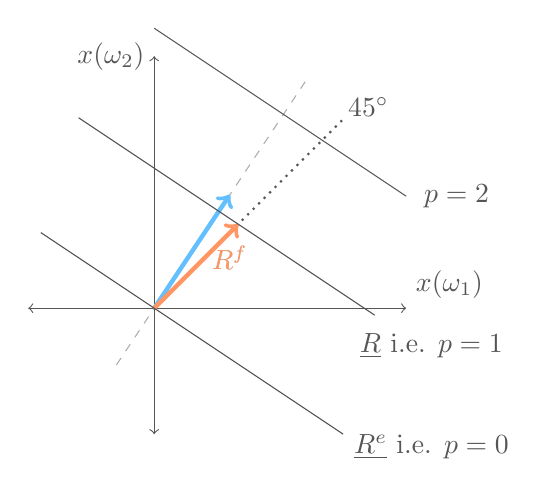
\begin{tikzpicture}[xscale=1.6, yscale=1.6] %, shorten >= 3pt
  % Axes
  \draw[d4black, <->] (0,-1) -- (0,0) -- (0,2)
                      node[left]{$x(\omega_2)$};
  \draw[d4black, <->] (-1,0) -- (0,0) -- (2,0)
                      node[above right]{$x(\omega_1)$};

  % Contingent claims price vector, pc = (0.6, 0.9)
  % Hence p = 0.6x1 + 0.9x2 => x2 = (10/9)p - (2/3) x1
  \draw[d4gray, dashed] (-0.3,-0.45) -- (1.2,1.8);
  \draw[d4blue, ultra thick, ->] (0.0,0.0) -- (0.6,0.9);
  \node[d4gray] at (0.5,1.05) {$\bsp\bsc$};
  \node[d4blue] at (0.5,1.05) {$\bsp\bsc$};

  % Risk free rate
  \draw[d4black, thick, dotted] (0.0,0.0) -- (1.5,1.5);
  \node[d4black] at (1.7,1.6) {$45^{\circ}$};
  \draw[d4orange, ultra thick, ->] (0.0,0.0) -- (0.6666666,0.6666666);
  \node[d4gray] at (0.6,0.4) {$R^f$};
  \node[d4orange] at (0.6,0.4) {$R^f$};

  % Space of excess returns, x2 = -(2/3) x1
  \draw[d4black, thin] (-0.9, 0.6) -- (1.5, -1.0);
  \node[d4black] at (2.2,-1.1) {$\underline{R^e}$ i.e. $p=0$};

  % Space of returns, x2 = (10/9) - (2/3) x1
  \draw[d4black, thin] (-0.6, 1.5111111) -- (1.75,-0.05555555);
  \node[d4black] at (2.2,-0.3) {$\underline{R}$ i.e. $p=1$};

  % Space of p=2, x2 = (10/9)*2 - (2/3) x1
  \draw[d4black, thin] (0.0, 2.2222222) -- (2,0.88888888);
  \node[d4black] at (2.4,0.888888888) {$p=2$};
\end{tikzpicture}
%\begin{align*}
  %pc &= (0.6, \; 0.9)\\
 %p &= 0.6x_1 +  0.9x_2 \\
  %x_2 &= \frac{10}{9}p - \frac{2}{3}x_1
%\end{align*}

We can also use vector geometry to understand $p=\E[mx]$, i.e.\ pricing
with SDF
\begin{align*}
  \bsm=(m(\omega_1),\ldots,m(\omega_S))\in\R^S
\end{align*}
instead of contingent claims prices $pc(\omega)$.
To do so, simply switch the underlying inner product and norm from
Euclidean to $L^2$:
\begin{align*}
  \langle x,y \rangle := \E[xy]
  \qquad
  \lVert x\rVert := \sqrt{\E[x^2]}
\end{align*}
%What's more, we even have a version of Expression~\ref{vectorprice}:
%\begin{align*}
  %\langle x,y \rangle
  %= \lVert y\rVert \times \lVert \proj(x|y)\rVert
%\end{align*}
\emph{However}, important note:
we will continue to draw vectors, visualize projections, and reason in
Euclidean space. We use this visual metapher \emph{even though} every
dot/inner product is really $\E[xy]$ underneath, involving RVs $x,y$
rather than vectors $\bsx,\bsy$.

For example, we update the picture to
\vspace{10pt}

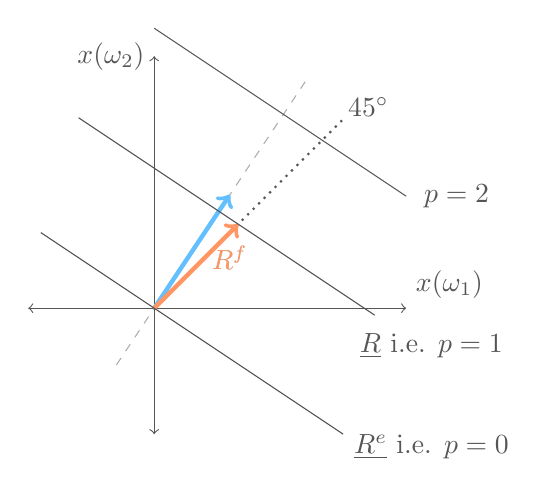
\begin{tikzpicture}[xscale=1.6, yscale=1.6] %, shorten >= 3pt
  % Axes
  \draw[d4black, <->] (0,-1) -- (0,0) -- (0,2)
                      node[left]{$x(\omega_2)$};
  \draw[d4black, <->] (-1,0) -- (0,0) -- (2,0)
                      node[above right]{$x(\omega_1)$};

  % Contingent claims price vector, pc = (0.6, 0.9)
  % Hence p = 0.6x1 + 0.9x2 => x2 = (10/9)p - (2/3) x1
  \draw[d4gray, dashed] (-0.3,-0.45) -- (1.2,1.8);
  \draw[d4blue, ultra thick, ->] (0.0,0.0) -- (0.6,0.9);
  \node[d4gray] at (0.5,1.05) {$\bsp\bsc$};
  \node[d4blue] at (0.5,1.05) {$\bsp\bsc$};

  % Risk free rate
  \draw[d4black, thick, dotted] (0.0,0.0) -- (1.5,1.5);
  \node[d4black] at (1.7,1.6) {$45^{\circ}$};
  \draw[d4orange, ultra thick, ->] (0.0,0.0) -- (0.6666666,0.6666666);
  \node[d4gray] at (0.6,0.4) {$R^f$};
  \node[d4orange] at (0.6,0.4) {$R^f$};

  % Space of excess returns, x2 = -(2/3) x1
  \draw[d4black, thin] (-0.9, 0.6) -- (1.5, -1.0);
  \node[d4black] at (2.2,-1.1) {$\underline{R^e}$ i.e. $p=0$};

  % Space of returns, x2 = (10/9) - (2/3) x1
  \draw[d4black, thin] (-0.6, 1.5111111) -- (1.75,-0.05555555);
  \node[d4black] at (2.2,-0.3) {$\underline{R}$ i.e. $p=1$};

  % Space of p=2, x2 = (10/9)*2 - (2/3) x1
  \draw[d4black, thin] (0.0, 2.2222222) -- (2,0.88888888);
  \node[d4black] at (2.4,0.888888888) {$p=2$};
\end{tikzpicture}

\clearpage
\subsubsection{Incomplete Markets}

Assume $\underline{X}\subsetneq \R^S$, i.e. tradeable assets don't
\emph{span} the state space. For ex, the figure below shows
$\dim(\underline{X})=2<S=3$. $\underline{X}$ is a plane extending out
from the triangle.

\vspace{10pt}
%\tdplotsetmaincoords{70}{15}
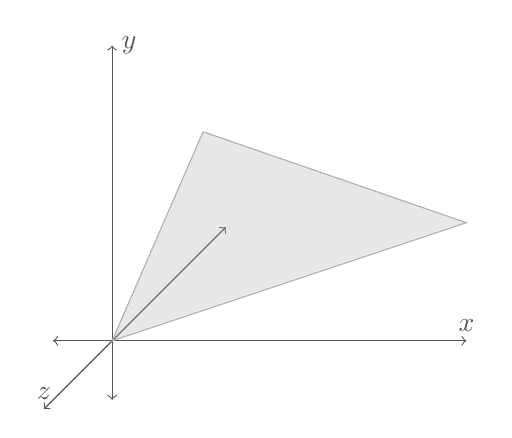
\begin{tikzpicture}[scale=1.5] %,tdplot_main_coords
    % Define axes
    \draw[d4black,<->] (-0.5,0,0) -- (3,0,0) node[above]{$x$};
    \draw[d4black,<->] (0,-0.5,0) -- (0,2.5,0) node[right]{$y$};
    \draw[d4black,<->] (0,0,-2.5) -- (0,0,1.5) node[anchor=south]{$z$};

    % Draw the plane
    \fill[
        draw=d4gray,%
        fill=d4gray,%
        fill opacity=0.3,%
    ] (0,1,-2)
      -- (3,1,0)
      -- (0,0,0)
      -- cycle;

    % Draw reference points
    %\node[d4black] at (0.7,0.7,1.8) {$b$};
\end{tikzpicture}
\\
\emph{Goal}: Suppose we don't have an economic model giving SDF $m$
pricing payoffs $x\in\underline{X}$ according to $p=\E[mx]$.
Can we go backwards and \emph{find} a SDF to price assets?

\begin{assump}
For all $x_1,x_2\in \underline{X}$ and $a,b\in\R$, we might assume
\begin{itemize}
  \item[A1.] \emph{Portfolio formation}:
    $ax_1+bx_2\in\underline{X}$.
  \item[A2.] \emph{Linearity/Law Of One Price} (LOOP):
    $p[ax_1+bx_2] = ap[x_1]+bp[x_2]$.
    \footnote{
      Note: people colloquially use ``no arb'' to refer to
      violations of A2/LOOP, \emph{not} A3 (which is stronger).
    }
  \item[A3.] \emph{No Arbitrage}:
    If $x(\omega)\geq x'(\omega)$ $\forall \omega\in\Omega$,
    strict for at least one $\omega$, $p[x]>p[x']$.

    With A1-2, equivalent to:
    If $x(\omega)\geq 0$ $\forall\omega$,
    strict for at least one, $p[x]>0$.
    (``No free assets that might pay'')
\end{itemize}
\end{assump}

\begin{thm}
We care about two directions
\begin{itemize}
  \item
    \emph{($\Rightarrow$)}
    Given SDF $m$ from an economic model pricing all assets/payoffs in
    $\R^S$ by $p=\E[mx]$, A2 (LOOP) holds.
  \item
    \emph{($\Leftarrow$)}
    Assuming A1 \& A2, $\exists\,!$ a discount factor
    $x^*\in\underline{X}$ pricing all assets in $\underline{X}$,
    i.e. s.t. $p=\E[x^*x]$ for all $x\in\underline{X}$
\end{itemize}
\end{thm}
\begin{proof}
($\Rightarrow$) $p[ax_1+bx_2] = \E[m(ax_1+bx_2)]$. Linearity of
$\E$ to conclude.

($\Leftarrow$) First, A1-2 imply \emph{parallel, linear} price
hyperplanes in $\underline{X}$.
Figure below depicts this for $\dim(\underline{X})=2$.
Dashed line $\perp$ to the price planes
pins down direction of $x^*$.
Then just fix length so $1=\E[x^*R]$ $\forall R\in\underline{R}$.

\vspace{10pt}

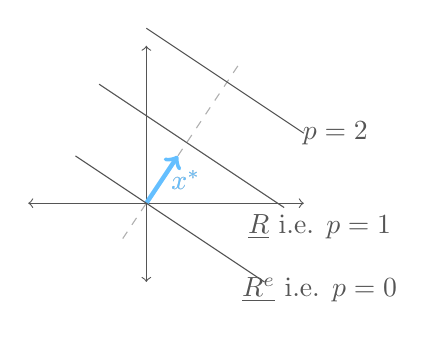
\begin{tikzpicture}[xscale=1, yscale=1] %, shorten >= 3pt
  % Axes
  \draw[d4black, <->] (0,-1) -- (0,0) -- (0,2);
  \draw[d4black, <->] (-1.5,0) -- (0,0) -- (2,0);

  % Contingent claims price vector, pc = (0.6, 0.9)
  % Hence p = 0.6x1 + 0.9x2 => x2 = (10/9)p - (2/3) x1
  \draw[d4gray, dashed] (-0.3,-0.45) -- (1.2,1.8);
  \draw[d4blue, ultra thick, ->] (0.0,0.0) -- (0.4,0.6);
  \node[d4gray] at (0.5,0.3) {$x^*$};
  \node[d4blue] at (0.5,0.3) {$x^*$};

  % Space of excess returns, x2 = -(2/3) x1
  \draw[d4black, thin] (-0.9, 0.6) -- (1.5, -1.0);
  \node[d4black] at (2.2,-1.1) {$\underline{R^e}$ i.e. $p=0$};

  % Space of returns, x2 = (10/9) - (2/3) x1
  \draw[d4black, thin] (-0.6, 1.5111111) -- (1.75,-0.05555555);
  \node[d4black] at (2.2,-0.3) {$\underline{R}$ i.e. $p=1$};

  % Space of p=2, x2 = (10/9)*2 - (2/3) x1
  \draw[d4black, thin] (0.0, 2.2222222) -- (2,0.88888888);
  \node[d4black] at (2.4,0.888888888) {$p=2$};
\end{tikzpicture}
\\
Algebra: If $\dim(\underline{X})=N\leq S$, can choose $N$ basis payoffs
in $\underline{X}$ that span. Stack these payoffs \& their prices
into vectors
$X(\omega):=(x_1(\omega)\ldots x_N(\omega))'$ and
$P:=(p_1\ldots p_N)'$

Since $x^*\in\underline{X}$ and assets in $X$ span $\underline{X}$, must
be $x^*=X'c$ for some weights $c$. Construct $c$ so $x^*$ prices basis
assets:
\begin{align*}
  P &= \E[x^*X] = \E[X(X'c)] = \E[XX']c
\end{align*}
We can solve for $c$ to get
\begin{align*}
  %\implies\;
  %c &= \E[XX']^{-1}P \\
  %\implies
  x^* &= P'\;\E[XX']^{-1}X
\end{align*}
Clearly, $x^*\in\underline{X}$, unique, prices assets in $X$ by
construction, and since they span $\underline{X}$, those assets can
replicate any other payoff in $\underline{X}$. So by A2, $x^*$ prices
everything else.
\end{proof}


\begin{cor}
Regarding unique $x^*\in \underline{X}$:
\begin{enumerate}[label=\emph{(\roman*)}]
  \item $\dim(\underline{X})=S$ implies $x^*$ unique in $\R^S$.
  \item $\underline{X}\subsetneq \R^S$ implies infinitely many
    SDFs that price all assets $x\in\underline{X}$ by
    formula $p=\E[\tilde{x}^*x]$ where
    \begin{align*}
      \tilde{x}^*
      = x^* + \varepsilon
      \;\;
      \text{where}\;
      \E[\varepsilon x] = 0,
      \; \forall x\in\underline{X}
    \end{align*}
  \item If $m$ is the unique, true SDF pricing all payoffs in $\R^S$,
    $x^*=\proj(m|\underline{X})$.
\end{enumerate}
\end{cor}

%Since $x^*\in\underline{X}$, it's clear that we might have
%$x^*(\omega)=0$ for some $\omega\in\Omega$.

\clearpage

Our next goal is to extend SDF $x^*\in\underline{X}$ (which prices
payoffs in $\underline{X}$) to ensure that we can \emph{also} price
payoffs in $\R^S\setminus\underline{X}$ \emph{without} implying
arbitrage opportunities.

While the last theorem guaranteed a unique $x^*\in\underline{X}$, it
did \emph{not} guarantee a \emph{strictly positive} $x^*$---and that's
\emph{key} for preventing arbitrage $\R^S\setminus\underline{X}$.
For example, suppose $\underline{X}\subsetneq\R^S$ is zero along
some axis. In other words, there exists a $\omega'\in\Omega$ such that
\begin{align*}
  x(\omega') = 0
  \qquad \forall x\in \underline{X}
\end{align*}
Then $x^*\in\underline{X}$ necessarily has $x^*(\omega')=0$.
But that could imply arbitrage opportunties (free portfolios that might
pay) if we try to price assets/payoffs \emph{outside} of
$\underline{X}$.

\begin{thm}
Again, two directions
\begin{itemize}
  \item \emph{($\Rightarrow$):}
    SDF $m$ from an economic model pricing all assets/payoffs
    in $\R^S$ by $p=\E[mx]$ plus A1 imply A2-3 hold.
  \item
    \emph{($\Leftarrow$):}
    Given A1-3, $\exists$ a
    \emph{strictly positive}\footnote{
      i.e. $m^*(\omega)>0$ for all $\omega\in\Omega$
    }
    SDF $m^*\in\R^S$ pricing all payoffs
    \begin{align*}
      p=\E[m^*x]
      \qquad
      \forall
      x\in \R^S\supseteq \underline{X}
    \end{align*}
    Note $m^*$ generally not unique or in $\underline{X}$ unless
    $\dim(\underline{X})=S$.
    Typically,
    \begin{align*}
      m^*=x^*+\varepsilon
      \;\text{where}\;
      \E[\varepsilon x]=0,\,
      \forall x\in\underline{X}
    \end{align*}
    All such SDFs agree about prices of
    $x\in\underline{X}$, generally disagree for
    $x\not\in\underline{X}$.
\end{itemize}
\end{thm}
\begin{proof}
($\Rightarrow$)
A2 holds by previous thm.
Since $m$ from economic model, it represents MU and is strictly
positive $m(\omega)>0$. Hence, for $x(\omega)\geq 0$ with $x(\omega')>0$
for at least one $\omega'$, clearly have $\E[mx]>0$, hence A3.
\\
\\
($\Leftarrow$)
A3/no-arb means any payoff in the nonnegative orthant of
$\R^S$ (excluding the origin) has positive price.
Again, there are parallel, linear price planes cutting through
$\underline{X}$.\footnote{%
  If $\dim(\underline{X})<S$, we have some freedom in the angle at which
  they cut through $\underline{X}$; otherwise, pinned down.
}
That includes the zero price plane, which intersects the nonnegative
orthant only at the origin. Thus $\exists$ a separating hyperplane
through the origin, separating the zero price hyperplane and
nonnegative orthant, with perpendicular vector pointing into the
positive orthant. This perpendicular vector pins down the direction of
$m^*$. To pin down length, simply normalize so it prices all returns
$1=\E[m^*R]$.
\end{proof}

\clearpage
\subsection{Representative Agent}

A representative agent is endowed with a marketable \emph{wealth portfolio}
that can be used to purchase consumption.
Into this wealth portfolio is capitalized \emph{everything} the agent
has that generates purchasing power: financial assets providing
dividends/returns, human capital generating labor income, etc.  This
wealth portfolio has current market value $W_t$ (in units of current
consumption $C_t$), i.e. one unit of the wealth portfolio can be traded
for one unit of consumption, and $W_t$ is max feasible
current consumption.

After consumption purchases, all remaining wealth $W_t-C_t$ is
reinvested to provide for future consumption, earning random
\emph{return on wealth} $R^W_{t+1}$ (which includes returns to financial
assets, returns to human capital aka labor income, etc.) that
generates additional purchasing power for the next period.
Hence, next period wealth $W_{t+1}$ satisfies intertemporal
budget constraint
\begin{align*}
  W_{t+1} = R_{t+1}^W(W_t-C_t)
\end{align*}
Defining $\tilde{W}_t:=W_t-C_t$, rearrange to get
\begin{align}
  R_{t+1}^W
  = \frac{W_{t+1}}{W_t-C_t}
  = \frac{\tilde{W}_{t+1}+C_{t+1}}{\tilde{W}_t}
  \label{retwealth0}
\end{align}
As the above discussion and Eq.~\ref{retwealth0} make clear, we can think
of the wealth portfolio simply as \emph{some asset} paying dividend
$C_{t+1}$ and with ex-dividend/ex-consumption price $\tilde{W}_{t}$ (in
units of $C_t$), cum-consumption price $W_t$, and \emph{return}
$R_{t+1}^W$.

\clearpage
\subsection{Exp. Return $\beta$ Rep}

\subsubsection{With Discount Factor, $m_t$}

Given discount factor $m$, Eqs~\ref{rf} \&~\ref{riskadjret} imply
\begin{align}
  \E[R^i]
  &=
  R^f +
  \frac{\Cov(m,R^i)}{\Var(m)}
  \left(
  -\frac{\Var(m)}{\E[m]}
  \right)
  \notag
  \\
  &=
  R^f +
  \underbrace{\beta_{i,m}}_{\substack{\text{Quantity}\\\text{of Risk}}}
  \times
  \underbrace{\lambda_m}_{\substack{\text{Price}\\\text{of Risk}}}
  \label{eq:betarep}
\end{align}
where $\beta_{i,m}$ is the population coefficient from a time series
regression of $R^i_t$ on $m_t$.

\subsubsection{With Reduced-Form Factors}

If we \emph{don't} have a discount factor $m$, we work backwards: we
model expected return $\E[R^i]$ for any asset $i$ as
\begin{align}
  %\text{(CS)}\;
  \E[R^i]
  = \gamma + \beta_{i,a}\lambda_a + \beta_{i,b} \lambda_b + \cdots
  %\qquad i = 1,\ldots,N
  \label{eq:expbetarep}
\end{align}
where the $\beta$'s are population coeffs from a time-series regression
of $R^i$ on some factors $f^a, f^b,\ldots$ that proxy for the SDF $m$
\begin{align}
  %\text{(TS)}\quad
  R_t^i = c_i + \beta_{i,a} f_t^a + \beta_{i,b} f_t^b + \cdots
  + \varepsilon^i_t
  %\qquad t = 1,\ldots,T
  \label{eq:getbetas}
\end{align}
We estimate the model in two regressions
\begin{enumerate}[label=(\roman*)]
  \item
    \emph{Time Series}:
    For each $i=1,\ldots,N$, estimate $\beta$'s (exposure to factors) by
    running Regression~\ref{eq:getbetas}
  \item
    \emph{Cross Section}:
    Given estimates $\hat{\beta}$ for each asset $i$ (now RHS
    variables), estimate risk/factor prices ($\lambda$'s)
    by reg
    \begin{align*}
      \frac{1}{T}\sumtT
      R^i_t
      = \gamma + \hat{\beta}_{i,a}\lambda_a + \hat{\beta}_{i,b}
      \lambda_b + \cdots
      + \alpha_i
    \end{align*}
\end{enumerate}
The $\alpha_i$'s from cross-sectional reg are errors/divergences
from the model's defining Equation~\ref{eq:expbetarep}. If the model is
exactly true (and no meas. error), the $\alpha_i$'s are exactly
zero.
\columnbreak

\emph{Factor Choice}: The factors are things that proxy for $m$ or,
equivalently, marginal utility (MU) growth---things like consumption
growth or the return on the market portfolio.
The factors $f_t^z$ are \emph{common} time-$t$ variables that depend
only on the underlying state of the economy. Factors \emph{cannot}
include firm/return/asset-$i$-specific characteristics like firm size or
form book-to-market.\footnote{%
  Though we could use average, economy-wide \emph{returns} to holding a
  portfolio of small or low book-to-market firms, since average
  returns to a specific portfolio offer information about the state of
  the economy broadly.
}
The factors $f^z_t$ are indexed by $t$, \emph{not} by $it$.

\emph{Zero-$\beta$ Rate, $\gamma$}:
In estimating the cross-sectional regression, we can impose restriction
$\gamma=R^f$ if the risk-free rate is observed in the market.
If not, we estimate $\gamma$ when running the cross-sectional.
We can ignore this issue entirely if we work strictly with excess
returns, in which case $\gamma$ is differenced out from
Eq~\ref{eq:expbetarep} and the cross-sectional regression to give model
\begin{align}
  \E[R^e]
  = \beta_{i,a}\lambda_a + \beta_{i,b} \lambda_b + \cdots
\end{align}

\emph{Returns as Factors}:
Suppose one of the factors is itself a return, wlog $f^a=R^a$.
Since Eq.~\ref{eq:expbetarep} holds for all returns, it must hold for
$R^a=f^a$ too. Then from Eq.~\ref{eq:getbetas}, $\beta_{a,a}=1$ and
$\beta_{a,z}=0$ for $z\neq a$.  Hence from Eq.~\ref{eq:expbetarep},
$\lambda_a=\E[R^a]-\gamma=\E[f^a]-\gamma$.

If all factors are excess returns, then the model can be written
\begin{align}
  %\text{(CS)}\;
  \E[R^{ei}]
  = \beta_{i,a}\E[f^a] + \beta_{i,b} \E[f^b] + \cdots
\end{align}
Can then estimate $\beta$'s by forming sample equivalents of $\E[R^e]$
and $\E[f^z]=\E[R^{ez}]$.


\clearpage
\subsection{Mean-Variance Frontier}

\subsubsection{With Discount Factor $m$}

Rewrite covariance in risk-adjustment Eq.~\ref{riskadjret}
\begin{align*}
  \E(R^i) - R^f
  &= -\frac{1}{\E(m)} \; \rho_{m,R^i} \; \sigma_{R^i} \; \sigma_m
\end{align*}
With corr $|\rho_{m,R^i}|\leq 1$,
letting $R^e=R^i-R^f$,
\begin{align*}
  \frac{\left\lvert\E(R^i) - R^f\right\rvert}{\sigma_{R^i-R^f}}
  =
  \frac{\left\lvert\E(R^e)\right\rvert}{\sigma_{R^e}}
  &\leq \frac{\sigma_m}{\E(m)}
\end{align*}
Thus expected excess returns for \emph{all} assets have \emph{bounded}
Sharpe Ratios and lie within a wedge-shaped
\emph{mean-variance frontier}.

\subsubsection{Incomplete Markets}

Given payoff space $\underline{X}\subseteq\R^S$, define subspaces of
returns \& excess returns (equivalently, the space of unit \& zero price
payoffs):
\begin{align*}
  \underline{R}
  &:=\{x\;|\; p[x]=1\}
  \quad
  \underline{R^e}
  :=\{x\;|\; p[x]=0\}
\end{align*}
Given unique SDF $x^*\in\underline{X}$ pricing assets $p=\E[x^*x]$,
define
\begin{align*}
  R^* &:=
  \frac{x^*}{p[x^*]}
  %= \frac{x^*}{\E[(x^*)^2]}
  \qquad
  R^{e*} :=
  \proj(1\;|\;\underline{R^e})
\end{align*}
Last line says $1 = R^{e*} + \varepsilon$ where
$\E[\varepsilon R^e]=0$ for all $R^e\in\underline{R^e}$.
Hence $R^{e*}$ represents \emph{mean} returns with an inner product the
way that $x^*$ represents prices with an inner product
\begin{align*}
  \E[R^e]
  =
  \E[1 \; R^e ]
  =
  \E[(R^{e*}+\varepsilon)R^e]
  %\\
  %\varepsilon\perp R^e\;
  %\implies\quad
  %\E[R^e]
  %&=
  =
  \E[R^{e*}R^e]
\end{align*}
In other words, as $p=\langle x^*, x \rangle$ for all
$x\in\underline{X}$, so too
$\E[R^e]=\langle R^{e*}, R^e \rangle$ for all $R^e\in\underline{R^e}$.

\begin{thm}
Can decompose any return
\begin{align*}
  R^i = R^* + w^i R^{e*} + n^i
\end{align*}
for some scalar $w^i\in\R$ and some excess return
$n^i\in\underline{R^e}$ that is mean zero $\E[n^i]=0$, with
all components mutually orthogonal:
\begin{align*}
  \E[R^*R^{e*}]
  =
  \E[R^*n^i]
  =
  \E[R^{e*}n^i]
  = 0
\end{align*}
\end{thm}
\begin{proof}
First, the constant \emph{price} hyperplanes running perpendicular to
$x^*$ also run perp to $R^*$, which is just $x^*$ stretched to hit
$\underline{R}$.

Next, constant \emph{mean} hyperplanes run perp to $R^{e*}$.
Note that any ${R^{e}}'\in\underline{R^e}$ such that
${R^{e}}'=R^e+\varepsilon$ and $\varepsilon\perp R^{e*}$
implies
\begin{align*}
  \E[R^{e*}{R^{e}}']
  =
  \E[R^{e*}(R^{e}+\varepsilon)]
  = \E[R^{e*}R^e]
\end{align*}
And since $\E[R^{e*}R^e]=\E[R^e]$
$\forall R^e,{R^e}'\in\underline{R^e}$, conclude that
$\E[{R^{e}}']=\E[R^{e}]$.

Algebra:
Given $R^*$, $R^{e*}$, define
\begin{align*}
  n^i = R^i - R^* -w^i R^{e*}
\end{align*}
Choosing $w^i$ so $n^i$ is indeed mean zero, we get
$w^i = (\E[R^i] - \E[R^*])/\E[R^{e*}]$.

With $R^*$, $R^{e*}$, and $n^i$ pinned down, just show orthogonality.
First, for any $R^e\in\underline{R^e}$
\begin{align*}
  \E[R^*R^e]=\E[x^*R^e]/p[x^*]=0
\end{align*}
$R^{e*}\in\underline{R^e}$ and $R^*,R^i\in\underline{R}$
imply $n^i,R^{e*}\in\underline{R^e}$ by construction and definition,
resp., so
\begin{align*}
  \E[R^*n_i]=\E[R^*R^{e*}]=0
\end{align*}
Lastly, $w^i$ was chosen so $\E[n^i]=0$, plus
$\E[R^{e*}R^e]=\E[R^e]$ for all $R^e\in\underline{R^e}$ (including
$n^i$). Hence, $0=\E[n^i] =\E[R^{e*}n^i]$.
\end{proof}

\clearpage
$R^*$ is also the minimum second moment return.


\clearpage
\section{Time-Series of Prices and Returns}

We discuss the following times-series facts for prices,
returns, dividends, \& $(P/D)$:
\begin{enumerate}
  \item \emph{Price Vol}: Prices vary \emph{a lot}. Why?
  \item \emph{Return \& Div. Growth Predictability}:
    Classical view wrong.
    Given $(P/D)$ ratio \emph{today}, can predict future \emph{returns}
    but \emph{not} future \emph{dividend growth}.
\end{enumerate}
As we will see, \emph{time-varying discount rates} explain both (1) \&
(2), which are really the same phenomenon becuase of PV identities

\subsection{Documenting Facts 1 \& 2}
\label{sec:predictability}

Fact 1: Stock prices move \emph{a lot} in the data relative to
dividends.  So big slow-moving swings in $(P/D)$ ratio are \emph{price}
swings.

Fact 2:
Test predictability of $k$-period returns or div. growth by time-series
regs on any arbitrary signal $X_t$ today:
\begin{align*}
  R_{t\ra t+k} &= a + bX_t + \varepsilon_t \\
  D_{t+k}/D_t &= c + dX_t + \varepsilon_t
\end{align*}

If $X_t=R_t$, $b\approx 0$ so
markets ``efficient'': current returns don't predict future returns.

If $X_t=(P/D)_t$, estimates contradict ``Classical
View''\footnote{%
  i.e. ``High $(P/D)$ implies dividend growth'' .
}
that $b=0$, $d=1$. Really
\begin{itemize}
  \item
    $d<0$, so high $(P/D)_t$ \emph{doesn't} forecast future div. growth.
    Wrong sign.
  \item
    $b\approx -1$, so
    high $(P/D)_t$ forecasts \emph{low} expected future returns.
    Also, $b$ and $R^2$ grow with horizon $k$,\footnote{%
      But mechanical since $P/D$ persistent.
      So nothing new beyond small-$k$ reg.
      Just highlights predictability
    }
    and exp. returns (fitted values $\hat{R}_{t\ra t+k}$) vary a
    lot, i.e.  $\sigma^2(\hat{R}_{t\ra t+k})$ large.
\end{itemize}
Hence $(P/D)$ \emph{today} forecasts future \emph{returns} and
\emph{not} future dividend growth.


\columnbreak
\subsection{Explaining Facts 1 \& 2}

\subsubsection{PV Identity, Fact 1 Intuition}

Start with ex-post realized return identity
\begin{align}
  R_{t+1}
  :=
  \frac{P_{t+1}+D_{t+1}}{P_t}
  \label{expostrealizedreturns}
\end{align}
Rearrange, take $\E_t$, solve forward,
\begin{align*}
  P_{t}
  = \E_t\left[\frac{P_{t+1}+D_{t+1}}{R_{t+1}}\right]
  =
  \E_t\sum_{s=1}^\infty
  \frac{D_{t+s}}{\prod_{k=1}^s R_{t+k}}
\end{align*}
This PV identity says price \emph{today} is exp. discounted future divs.
Together with Fact 1 (i.e. that prices vary), two implications:
\begin{itemize}
  \item We don't live in world with iid or constant returns and dividend
    growth.
  \item
    \emph{Either} exp future \emph{dividends} or \emph{returns}
    time-vary. Need data to pick which.
\end{itemize}
But because the above PV formula involves nonstationary $P_t$ \& $D_t$
and is nonlinear in (generally time-varying) returns and dividends, it's
tough to work with. However, we can obtain a log-linear approximation
that's much easier to work with. This is the topic of the next
subsection.

As a side note, the special case where the above PV formula \emph{is}
easy to work with follows if we assume constant returns and dividend
growth: $R_{t+s}=R$ and $D_{t+s}=G^sD_t$ with $G<R$. Then the above PV
formula simplifies to the \emph{Gordon Growth} formula
\begin{align*}
  P_{t}
  =
  \E_t\sum_{s=1}^\infty
  \frac{G^sD_{t}}{R^s}
  =
  \frac{1}{1-\left(\frac{G}{R}\right)}
  \approx
  \frac{1}{r-g}
\end{align*}
where $r=\ln R$ and $g=\ln G$, which implied approximation
$G/R\approx 1+g-r$.



\columnbreak
\subsubsection{Shiller-Campbell PV Ident.}

We now derive an alternative PV identity that's both log-\emph{linear}
and written in terms of generally stationary variables.
Start by rewriting Eq.~\ref{expostrealizedreturns}:
\begin{align*}
  R_{t+1}
  %= \frac{P_{t+1}+D_{t+1}}{P_t}
  =
  \frac{D_{t+1}}{D_t}
  \frac{D_{t}}{P_t}
  \left(
  1+
  \frac{P_{t+1}}{D_{t+1}}
  \right)
\end{align*}
Take logs, let lower case denote logs, and define log price-dividend
ratio $pd_t:=p_t-d_t$:
\begin{align}
  r_{t+1}
  =
  \Delta d_{t+1} - pd_t + \ln\big( 1+ e^{pd_{t+1}} \big)
  \label{shillerprelog}
\end{align}
Let $f(pd_{t+1}):=\ln(1+e^{pd_{t+1}})$, log-linearize
about unconditional average $pd:=\E[pd_t]$
\begin{align*}
  %f(pd_{t+1})
  \ln(1+e^{pd_{t+1}})
  &\approx
  f(pd) + f'(pd)(pd_{t+1}-pd)
  \\
  &=
  \ln(1+e^{pd})
  +
  \rho
  %\frac{e^{pd}}{1+e^{pd}}
  (pd_{t+1}-pd)
\end{align*}
where $\rho:=\frac{e^{pd}}{1+e^{pd}}$.
Substitute this approximation back into original
Expression~\ref{shillerprelog}, drop additive constants to arrive at
\begin{align*}
  r_{t+1}
  &\approx \Delta d_{t+1} - pd_t + \rho \; pd_{t+1}
\end{align*}
Rearrange to put $pd_t$ on the LHS:
\begin{align}
  pd_t
  =
  %\E_t\big[
    \Delta d_{t+1}- r_{t+1} + \rho \; pd_{t+1}
  %\big]
  \label{pdidentity}
\end{align}
Solve forward $k$ periods
\begin{align}
  pd_t = \rho^kpd_{t+k}
  +\sum_{s=1}^k \rho^{s-1}\big(\Delta d_{t+s}-r_{t+s}\big)
  \label{pdidentityk}
\end{align}
Send $k\ra \infty$ and impose ``no bubbles'' (so that the last term goes
to zero) to get
\begin{align}
  \boxed{%
  pd_t
  =
  \sum_{s=1}^\infty
  \rho^{s-1}\big(\Delta d_{t+s}-r_{t+s}\big)
  }
  \label{pdidentityinf}
\end{align}
This nice, linear PV identity in stationary variables is ideal for
taking to the data.

Lastly, note that, as they stand now now,
Expressions~\ref{pdidentity}-\ref{pdidentityinf} are ex post identities,
but we can always always take $\E_t$ of both sides to get an ex ante
statement.


\columnbreak
In fact, it is often useful to look at the \emph{surprise} or
\emph{innovation} in a variable, so define the expectation-difference
operator
\begin{align*}
  \Delta \E_{t+1}[z_s]
  := (\E_{t+1} - \E_{t})[z_s]
  = \E_{t+1}[z_s] - \E_{t}[z_s]
\end{align*}
We use this operator to look at the the difference between realization
and expectation:
$\Delta \E_{t+1}[z_{t+1}]=z_{t+1}-\E_{t}z_{t+1}$.


With this, rewrite Expr.~\ref{pdidentityinf} by applying $\Delta
\E_{t+1}$ to both sides, and rearrange to get
\begin{align}
  \Delta\E_{t+1}r_{t+1}
  &=
  \Delta \E_{t+1} \sum_{s=0}^\infty \rho^{s}\Delta d_{t+1+s}
  \notag
  \\
  &\quad
  -\Delta \E_{t+1} \sum_{s=1}^\infty \rho^{s}r_{t+1+s}
  \label{rsurprise}
\end{align}
%or, equivalently, the formula
%\begin{align}
  %\Delta\E_{t+1}r_{t+1}
  %&=
  %\Delta \E_{t+1}\Delta d_{t+1}
  %- \Delta \E_t \sum_{s=1}^\infty \rho^{s}r_{t+1+s}
  %\notag
  %\\
  %&
  %+ \Delta \E_{t+1} \sum_{s=1}^\infty \rho^{s}\Delta d_{t+1+s}
  %\label{rsurprise}
%\end{align}


\subsubsection{Campbell-Mankiw Identity}

%Recall that the representative agent's cum-consumption wealth
%$W_t=\tilde{W}_t+C_t$ satisfies the intertemporal budget constraint
%\begin{align}
  %R_{t+1}^W
  %= \frac{W_{t+1}}{W_t-C_t}
  %\label{retwealth}
%\end{align}
Thinking of wealth as an asset with cum-consumption/cum-dividend price
$W_t$ and dividends $C_t$, we can just as well derive a Campbell-Shiller
PV identity for this asset, as for any other asset:
\begin{align}
  \boxed{%
  c_t-w_t
  = \sum_{s=1}^\infty \rho^s (r^w_{t+s}-\Delta c_{t+s})
  }
  \label{wcidentityinf}
\end{align}
We can also apply $\Delta\E_{t+1}$ to both sides of the above and
rearrange to decompose the ``surprise'' in consumption at $c_{t+1}$ into
changes in expected future return on the wealth portfolio and changes in
expected future consumption growth:
\begin{align}
  \Delta \E_{t+1}\Delta c_{t+1}
  &=
  \Delta \E_{t+1}\sum_{s=1}^\infty \rho^s r^w_{t+s}
  \notag
  \\
  &- \Delta \E_{t+1}\sum_{s=2}^\infty \rho^s \Delta c_{t+s}
  \label{csurprise}
\end{align}
%Notice also $\Delta c_{t+1}-\E_t\Delta
%c_{t+1}=c_{t+1}-\E_tc_{t+1}$. And we can also pop off the first term of
%the first sum to reexpress the above as
%\begin{align}
  %\Delta c_{t+1}-\E_t\Delta c_{t+1}
  %&=
  %r^w_{t+1}-\E_tr_{t+1}^w
  %\notag
  %\\
  %&
  %+
  %\big(\E_{t+1}-\E_t\big)\sum_{s=2}^\infty \rho^s r^w_{t+s}
  %\notag
  %\\
  %&- \big(\E_{t+1}-\E_t\big)\sum_{s=2}^\infty \rho^s \Delta c_{t+s}
  %\label{wcidentitE2}
%\end{align}
%Again, the surprise in consumption due to realized surprise in returns,
%expected future returns, and exp future consumption growth.



\columnbreak
\subsubsection{Decomposing $Var(pd_t)$}
\label{sec:decompvar}

Apply operator $\Cov(pd_t,\cdot)$ to both sides of
Expression~\ref{pdidentityinf} to get
\begin{align}
  \Var(pd_t)
  &=
  \Cov\left(
    pd_t,\;
    \sum_{s=1}^\infty \rho^{s-1}\Delta d_{t+s}
  \right)
  %\label{decomppd}
  \notag
  \\
  &\;\;
  -
  \Cov\left(
    pd_t,\;
    \sum_{s=1}^\infty \rho^{s-1}r_{t+s}
  \right)
  \notag
\end{align}
If you divide both sides of this last expression by $\Var(pd_t)$,
you get $1=\beta_{1}-\beta_{2}$, i.e. difference of population
regression coefficients
\begin{align*}
  \sum_{s=1}^\infty \rho^{s-1}\Delta d_{t+s}
  &= \alpha_{1} + \beta_{1}\; pd_t
  + \varepsilon^{1}_t
  \\
  \sum_{s=1}^\infty \rho^{s-1}r_{t+s}
  &= \alpha_{2} + \beta_{2}\; pd_t + \varepsilon^2_t
\end{align*}
And this is really neat because
\begin{enumerate}
  \item
    The regression coefficients decompose $\Var(pd_t)$, with
    $\beta_{1}$ and $\beta_2$ representing the \emph{share} of
    $\Var(pd_t)$ explained by changes in expected future dividends and
    discount rates, respectively.

  \item
    These regressions are more or less \emph{the same} as those we ran
    in Section~\ref{sec:predictability} (they just used a finite-time,
    equally weighted approximation of the LHS here).
    And we already know $\beta_{1}\approx 0$, $\beta_2\approx -1$.
    Hence, volatility in $pd_t$ is \emph{entirely} driven by changes in
    exp. future discount rates.

  \item
    Hence, Fact 2 predictability \emph{intimately linked} with Fact 1
    volatility, as shown by this decomposition.
    It's the \emph{same} underlying phenomenon.
\end{enumerate}
So Shiller's ``excess volatility'' in prices (relative to
dividends) is just \emph{discount rates} moving much more than
dividends.

\subsubsection{Decomposing Surprise, $\Var(\Delta \E_t r_t)$}
\label{sec:decompsur}

Take Eq~\ref{rsurprise} at $t$ (rather than $t+1$), and pop off the
first term in the first sum to get equivalent decomposition
\begin{align*}
  \Delta\E_{t}r_{t}
  &=
  \Delta\E_t\Delta d_t
  + \Delta \E_{t} \sum_{s=1}^\infty \rho^{s}\Delta d_{t+s}
  \notag
  \\
  &\quad
  -\Delta \E_t \sum_{s=1}^\infty \rho^{s}r_{t+s}
\end{align*}
Thuse we can decompose the variance of the surprise in realized $r_t$
today into contributions from surprise in dividends today, changes in
exp.  of future dividend  growth, and changes in expectations of future
interest rates (plus a final cov term):
\begin{align}
  &\Var(\Delta\E_tr_t)
  =
  \Cov\left(
    \Delta \E_{t}r_{t},\;
    \Delta \E_{t}\Delta d_{t}
  \right)
  \label{decompsurprise}
  \\
  &\;\;\;
  +\Cov\left(
    \Delta \E_{t}r_{t},\;
    \Delta \E_{t}
    \sum_{s=1}^\infty
    \rho^{s}\Delta d_{t+s}
  \right)
  \notag
  \\
  &\;\;\;
  -\Cov\left(
    \Delta \E_{t}r_{t},\;
    \Delta \E_{t}
    \sum_{s=1}^\infty
    \rho^{s}r_{t+s}
  \right)
  \notag
  \\
  &\;\;\;
  +2\Cov\left(
    \Delta \E_{t}
    \sum_{s=1}^\infty
    \rho^{s}\Delta d_{t+s}
    ,\;
    \Delta \E_{t}
    \sum_{s=1}^\infty
    \rho^{s}r_{t+s}
  \right)
  \notag
\end{align}
Divide through by $\Var(\Delta \E_tr_t)$, and the first three terms are
coeffs from time-series regs
\begin{align*}
  \Delta \E_{t}\Delta d_{t}
  &=
    \tilde{\alpha}_{1}
    + \tilde{\beta}_{1} \; (\Delta \E_{t}r_{t})
    + \nu_t^{1} \\
  \Delta \E_{t}
  \sum_{s=1}^\infty
  \rho^{s}\Delta d_{t+s}
  &=
    \tilde{\alpha}_{2}
    + \tilde{\beta}_{2} \; (\Delta \E_{t}r_{t})
    + \nu_t^{2} \\
  \Delta \E_{t}
  \sum_{s=1}^\infty
  \rho^{s}r_{t+s}
  &=
    \tilde{\alpha}_{3}
    + \tilde{\beta}_{3} \; (\Delta \E_{t}r_{t})
    + \nu_t^{3}
\end{align*}
We find $\tilde{\beta}_1\approx 0.5$, $\tilde{\beta}_2\approx 0$, and
$\tilde{\beta}_3\approx 0.5$.


\columnbreak
\subsection{VAR Estimation}

To estimate regression coefficients associated with the variance
decompositions of Sections~\ref{sec:decompvar} and \ref{sec:decompsur},
we could (as suggested) estimate each time-series regression equation
separately, approximating infinite sums with finite sums.
Note that generally, one regression is redundant, since the reg
coefficients \emph{must} add up because of the PV restrictions we
derived from Expr~\ref{pdidentity}.

\emph{Alternatively}, we can specify a VAR for the joint evolution of
$(r_t,\Delta d_t,pd_t)$.
Then we can easily compute covariances with infinite sums of
conditional expectations like $\sum_{s=1}\rho^{s-1}\E_tr_{t+s}$ by using
the VAR to generate forecasts/expectations.\footnote{%
  Of course, specifying a stationary fixed-param VAR runs the risk
  of structural breaks, non-stationarity, and other extrapolation
  dangers. By using stationary $pd_t$ rather than nonstationary $p_t$,
  we've tried to avoid the most egregious problem. But there's still
  risks.
}
We just also need to impose PV Restriction~\ref{pdidentity} so that
long-horizon projections computed from this VAR respect that identity
and are thus valid.


\subsubsection{Model Specification, Est.}

Define $\bsx_t:=(r_t,\Delta d_t,pd_t)$ and let
\begin{align}
  \bsx_t &= \bsPhi \bsx_{t-1} + \bsvarepsilon_t
  \qquad\E[\bsvarepsilon_t\bsvarepsilon_t'] = \bsSigma
  \label{pdvar}
\end{align}
Given model parameters $\bsPhi$ and $\bsSigma$, can then also define and
compute $\bsGamma := \E[\bsx_t\bsx_t']$ as
\begin{align*}
  \bsGamma
  =
  \vc^{-1}\big(
  (\bsI-\bsPhi\otimes\bsPhi)^{-1}
  \vc(\bsSigma)
  \big)
\end{align*}
Letting $\bse_i$ denote the $i$th basis element, we can write
Restriction~\ref{pdidentity} in terms of state vector $\bsx_t$ and
parameters as
\begin{align}
  \bse_3'
  =
  \big(\bse_2' - \bse_1' + \rho\bse_3' \big) \bsPhi
  \label{pdvarrestrict}
\end{align}
We then estimate Model~\ref{pdvar} via GMM with moment condition
\begin{align*}
  \bsg_t(\bsPhi)
  = \bsvarepsilon_t \otimes \bsx_{t-1}
  = (\bsx_t-\bsPhi \bsx_{t-1})\otimes \bsx_{t-1}
\end{align*}
subject to linear parameter restriction~\ref{pdvarrestrict}.


\subsubsection{$\Var(pd_t)$ Decomposition}

Similar to the Sec.~\ref{sec:decompvar} decomp, apply $\Cov(pd_t,\cdot)$
to both sides of Eq.~\ref{pdidentityk} to get
\begin{align*}
  \Var(pd_t)
  &=
  \Cov(
      pd_t,
      %\underbrace_{=:\;pd_t(k)}
      )
  \\
  &\quad
  +\Cov\bigg(
    pd_t,\;
    %\underbrace_{=:\;\Delta d_t(k)}
  \bigg)
  \\
  &\quad-
  \Cov\bigg(
    pd_t,\;
    %\underbrace_{=:\;r_t(k)}
  \bigg)
\end{align*}
We can rewrite this in terms of VAR params:
\begin{align*}
  \bse_3'\bsGamma\bse_3
  &=
  %\Cov\left(
    %pd_t,\;
    %\Delta d_t(k)
  %\right)
  %&=
  %\Cov\left(
    %\bse_3'\bsx_t,\;
    %\sum_{s=1}^k \rho^{s-1}
    %\bse_2'\bsx_{t+s}
  %\right)
  %\\
  %&=
  %\Cov\left(
    %\bse_3'\bsx_t,\;
    %\sum_{s=1}^k \rho^{s-1}
    %\bse_2'\bsPhi^s\bsx_t
  %\right)
  %\\
  %&=
  %\Cov\left(
    %\bse_3'\bsx_t,\;
    %\rho^{-1}\bse_2'
    %\sum_{s=1}^k
    %(\rho\bsPhi)^s\bsx_t
  %\right)
  %\\
  %&=
  %\Cov\left(
    %\bse_3'\bsx_t,\;
    %\bse_2'
    %\bsPhi(\bsI-(\rho\bsPhi)^k)(\bsI-\bsPhi)^{-1}
    %\bsx_t
  %\right)
  %\\
  %&=
  %\bse_2'
  %\bsPhi(\bsI-(\rho\bsPhi)^k)(\bsI-\bsPhi)^{-1}
  %\Cov\left(
    %\bsx_t
    %,\;
    %\bsx_t
  %\right)
  %\bse_3
  %\\
  \bse_3'
  (\rho\bsPhi)^k\bsGamma
  \bse_3
  \\
  &\;\;\;
  + \bse_2'
  \bsPhi(\bsI-(\rho\bsPhi)^k)(\bsI-\rho\bsPhi)^{-1}
  \bsGamma
  \bse_3
  \\
  &\;\;\;
  - \bse_1'
  \bsPhi(\bsI-(\rho\bsPhi)^k)(\bsI-\rho\bsPhi)^{-1}
  \bsGamma
  \bse_3
\end{align*}

\subsubsection{$\Var(\Delta \E_t r_t)$ Decomposing}

We will do a slightly different, more convenient decomp.
So rewrite Expr.~\ref{rsurprise} as
\begin{align*}
  \Delta\E_tr_{t}
  =
  \Delta \E_t \sum_{s=0}^\infty \rho^{s}\Delta d_{t+s}
  - \Delta \E_t \sum_{s=1}^\infty \rho^{s}r_{t+s}
\end{align*}
In terms of VAR objects, can write this
\begin{align*}
  \bse_1'\bsvarepsilon_t
  &=
  \sum_{s=0}^\infty \bse_2'(\rho\bsPhi)^{s}\bsvarepsilon_t
  - \sum_{s=1}^\infty \bse_1'(\rho\bsPhi)^{s}\bsvarepsilon_t
  \\
  &=
  \bse_2'
  (\bsI-\rho\bsPhi)^{-1}
  \bsvarepsilon_t
  -\bse_1'\rho\bsPhi
  (\bsI-\rho\bsPhi)^{-1}
  \bsvarepsilon_t
\end{align*}
Compute covariance of this with
$\Delta\E_tr_t=\bse_1'\bsvarepsilon_t$ to get a variance decomposition
like Expression~\ref{decompsurprise} in terms of model parameters:
\begin{align*}
  \bse_1'\bsSigma\bse_1
  &=
  \bse_2'
  (\bsI-\rho\bsPhi)^{-1}
  \bsSigma
  {(\bsI-\rho\bsPhi)^{-1}}'
  \bse_2
  \\
  &
  +\rho^2\bse_1'\bsPhi
  (\bsI-\rho\bsPhi)^{-1}
  \bsSigma
  {(\bsI-\rho\bsPhi)^{-1}}'
  \bsPhi'\bse_1
  \\
  &
  -
  2\rho
  \bse_1'
  \bsPhi
  (\bsI-\rho\bsPhi)^{-1}
  \bsSigma
  {(\bsI-\rho\bsPhi)^{-1}}'
  \bse_2
\end{align*}
On RHS, first term is contribution from surprise in current divs and
changes in exp future divs.
Second from changes in exp future discount rates.
Third from covariance between these two sources.


\clearpage
\section{Consumption-Based Asset Pricing}

\subsection{Portfolio Choice FOCs}

There are essentially two FOCs that characterize the entire portfolio
choice problem wherein the agent chooses an optimal portfolio and level
of consumption:
\begin{enumerate}
  \item Returns, $\forall i$: $1=\E_t[M_{t+1}R_{t+1}^i]$
  \item SDF:
    An equation defining the SDF, which pins down consumption through
    $1=\E_t[M_{t+1}R_{t+1}^w]$, where $R_{t+1}^w$ is the return on the
    wealth portfolio.

    The exact expression for the SDF depends on the functional form of
    utility.
    \begin{itemize}
      \item CRRA:
        $M_{t+1}=\beta\left(\frac{C_{t+1}}{C_t}\right)^{-\gamma}$
      \item EZ:
    \end{itemize}
\end{enumerate}
Takeing returns $R^n_{t+1}$ as given,
the rep agent chooses portfolio weights $B_t^n$ to maximize recursive
Epstein-Zin utility with EIS $\sigma$ and risk-aversion parameter
$\gamma$, subject to an intertemporal budget constraint,
\begin{align*}
  U_t
  &=
  \left(
  (1-\beta)c_t^{1-\frac{1}{\sigma}}
  + \beta
  \E_t\left[U_{t+1}^{1-\gamma}\right]^{\frac{1-\frac{1}{\sigma}}{1-\gamma}}
  \right)^{\frac{1}{1-\frac{1}{\sigma}}}
  \\
  \text{s.t.}\quad&
  W_{t+1}
  =
  \sum_{n=0}^N B_t^n R_{t+1}^n
  =
  R^W_{t+1}(W_t-C_t)
\end{align*}
where $\kappa := \frac{1-\gamma}{1-1/\sigma}$.
This has FOCs:
\begin{align}
  1 &= \E_t[M_{t+1}R_{t+1}^n]
  \quad \forall n
  \label{ccapmfoc}
  \\
  \text{where}\quad
  M_{t+1}
  &=
  \left[
  \beta \left(
  \frac{C_{t+1}}{C_t}
  \right)^{-\frac{1}{\sigma}}
  (R^W_{t+1})^{1-\frac{1}{\kappa}}
  \right]^\kappa
  \notag
\end{align}
Supposing $\beta=e^{-\delta}$, the log SDF is
\begin{align}
  m_{t+1}
  &=
  -\kappa
  \delta
  -
  \frac{\kappa}{\sigma}
  \Delta c_{t+1}
  +
  \left(
  \kappa-1
  \right)
  r^w_{t+1}
  %\notag
  \label{logsdf}
\end{align}
We now derive two useful approximations given any joint dist for
$(M_{t+1},R_{t+1}^n)$.
First, a first order log-linear approx of Eq.~\ref{ccapmfoc} gives:
\begin{align}
  1
  &=
  \E[e^{m_{t+1}+r_{t+1}^n}]
  \approx e^{\E_tm_{t+1}+\E_tr^n_{t+1}}
  \notag
  %\\
  %\iff\quad
  %0&\approx \E_tm_{t+1}+\E_tr^n_{t+1}
\end{align}
Taking logs, setting $r_{t+1}^n=r_{t+1}^w$, and using
Expression~\ref{logsdf}, this implies:
\begin{align}
  \boxed{
  \frac{1}{\sigma}\E_t\Delta c_{t+1}
  =
  - \delta + \E_tr_{t+1}^w
  }
  \label{ezeuler}
\end{align}
Second, we can also use Eq.~\ref{ccapmfoc} to derive
\begin{align*}
  &\E[R_{t+1}^n-R_{t+1}^f]
  \\
  &\quad
  =
  \Cov_t\left(
  -\frac{M_{t+1}}{\E_t[M_{t+1}]},
  \;R_{t+1}^n-R_{t+1}^f
  \right)
  %\\
  %&\quad
  %\approx
  %\Cov_t\left(
  %-m_{t+1},
  %\;R_{t+1}^n-R_{t+1}^f
  %\right)
\end{align*}
Sub in approx $m_{t+1}\approx M_{t+1}/\E_t[M_{t+1}]$, use
Eq.~\ref{logsdf}, and simplify to get an expression for the
risk-premium:
\begin{align*}
  \E[R_{t+1}^n-R_{t+1}^f]
  &\approx
  \frac{\kappa}{\sigma}\Cov_t\left(
  \Delta c_{t+1},\;
  \;R_{t+1}^n-R_{t+1}^f
  \right)
  \\
  &
  +(1-\kappa)
  \Cov_t\left(
  r_{t+1}^w,
  \;R_{t+1}^n-R_{t+1}^f
  \right)
\end{align*}
Notice Epstein-Zin utility lies in between the consumption CAPM
($\kappa=1$, all weight on cov with consumption) and the usual
CAPM ($\kappa=0$, all weight on cov with the market/wealth portfolio).



\subsection{Assuming Lognormality}

Assuming joint lognormality of $(m_{t+1},r_{t+1}^n)$, we get even nicer
\emph{exact} formulas.  Specifically, FOC~\ref{ccapmfoc} becomes
\begin{align}
  0 &=
  \E_t\big[m_{t+1}+r_{t+1}^n\big]
  +
  \frac{1}{2}\Var_t\big(
  m_{t+1}+r_{t+1}^n\big)
  \notag
  %\label{foclognormal}
\end{align}
Use Eq.~\ref{logsdf} to evaluate this when $r^n_{t+1}=r^f_{t+1}$ and
$r^w_{t+1}$, then solve for $r^f_{t+1}$ to get
\begin{align*}
  r_{t+1}^f
  =
  \delta
  +\frac{1}{\sigma}\E_t\Delta c_{t+1}
  &-
  \frac{\kappa}{2\sigma^2}
  \Var_t(\Delta c_{t+1})
  \\
  &
  +
  \frac{\kappa-1}{2}
  \Var_t(r_{t+1}^w)
\end{align*}
Then again use the lognormal FOC with Eq~\ref{logsdf} to derive the
\emph{exact} risk premium for any return $r_{t+1}^n$:
\begin{align*}
  &\E_t[r_{t+1}^n - r^f_{t+1}]
  +\frac{1}{2}
  \Var_t\big(r_{t+1}^i\big)
  \\
  &
  \qquad\quad
  =
  \frac{\kappa}{\sigma}
  \Cov_t\left(\Delta c_{t+1},\; r_{t+1}^i\right)
  \\
  &
  \qquad\quad\quad
  +(1-\kappa)\Cov_t\left( r_{t+1}^w,\; r_{t+1}^i\right)
\end{align*}
Notice from these formulas: $r^f_{t+1}$ depends \emph{only} on IES
$\sigma$, \emph{not} risk aversion parameter $\gamma$, which does show
up in the expression for the risk premium. Therefore, we can choose
$\sigma$ to nail the behavior of $r^f_{t+1}$ and, at the same time, dial
up $\gamma$ to match the risk premium.



\subsection{Intertemporal CAPM}

Want consumption out of the model. To start, recall
Identity~\ref{csurprise}:
\begin{align*}
  \Delta \E_{t+1}\Delta c_{t+1}
  &=
  \Delta \E_{t+1}\sum_{s=1}^\infty \rho^s r^w_{t+s}
  \notag
  \\
  &- \Delta \E_{t+1}\sum_{s=2}^\infty \rho^s \Delta c_{t+s}
\end{align*}
Use approximate Euler Eq.~\ref{ezeuler} to substitute out
$\Delta c_{t+s}$ on the RHS, then regroup to get
\begin{align*}
  \Delta \E_{t+1}\Delta c_{t+1}
  &=
  \Delta \E_{t+1}r_{t+1}^w
  \\
  &\quad
  + (1-\sigma)\Delta\E_{t+1}\sum_{s=2}^\infty \rho^s r^w_{t+s}
  \notag
\end{align*}
Notice that surprises in current wealth return affect consumption
one-for-one, while the additional term captures changes in expected
future wealth returns.
Only if $\sigma=1$ do income and substitution effects ofset.

Sub this last formula in on the RHS for $\Delta c_{t+1}$ in the
approximate expression for the risk-premium\footnote{%
  This is valid because
  $\Cov_t(c_{t+1},\cdot)=\Cov_t(c_{t+1}-\E_tc_{t+1},\cdot)
  =\Cov_t(\Delta
  \E_{t+1}c_{t+1},\cdot)$
}
and simplify (recalling $\kappa=(1-\gamma)/(1-1/\sigma)$) and dropping
constant $R^f_{t+1}$ form the covariance:
\begin{align*}
  &\E_t[R_{t+1}^n-R_{t+1}^f]
  \approx
  \gamma
  \Cov_t\left(
  r^w_{t+1},
  R_{t+1}^n
  \right)
  \\
  &\;
  +
  (\gamma-1)
  \Cov_t\left(
  \Delta \E_{t+1}\sum_{s=2}^\infty \rho^s r^w_{t+s},
  R_{t+1}^n
  \right)
\end{align*}
This is the intertemporal CAPM. The first term is the usual CAPM
component. The second term captures covariance changing investment
opportuntities, i.e. changes in expected future wealth returns.

Lastly, Identity \ref{rsurprise} to sub in for $r^w_{t+1}$ in the first
covariance term and regroup
\begin{align*}
  &\E_t[R_{t+1}^n-R_{t+1}^f]
  \approx
  \\
  &\;
  \Cov_t\left(
  -\Delta\E_{t+1}\sum_{s=2}^\infty \rho^s r^w_{t+s},
  R_{t+1}^n
  \right)
  \\
  &\;
  +\gamma
  \Cov_t\left(
  \Delta \E_{t+1} \sum_{s=0}^\infty \rho^{s}\Delta d_{t+1+s}^w
  ,\;
  R_{t+1}^n
  \right)
\end{align*}
This decomposes expected excess returns into cash flow and discount rate
effects.

\clearpage
\section{Production}

Firms have operating profits $\Pi_t = Y_t - W_tL_t$. They pay out
dividends equal to profits less the cost of investments
\begin{align*}
  D_t = \Pi_t - \Phi_t
\end{align*}
where $\Phi_t$ is some adjustment cost based on initial capital $K_t$
and investment $I_t$.
The firm maximizes profits
\begin{align*}
  V_t = \max \E_t\sumsinfz M_{t,t+s} D_{t+s}
\end{align*}
The firm therefore solves
\begin{align*}
  V_t = \max D_t + \E_t M_{t+1} V_{t+1}
\end{align*}
subject to the rule for dividends and adjustment costs.





\clearpage
\section{Heterogeneous Agents}

\subsection{Constantinides and Duffie}

Let $Y_t$ be aggregate income, and assume that agents receive
a share $c_t(i)$ of idiosyncratic income, with time-varying
heteroskedasticity:
\begin{align*}
  C_t(i) &= c_t(i) Y_t \\
  \text{where}\quad
  \Delta \ln c_{t+1}(i)
  &= \eta_{t+1}(i) z_{t+1} - \frac{z^2_{t+1}}{2}
\end{align*}
where $\eta_{t+1}(i)\sim \calN(0,1)$ and $z_t$ is the amount of
idiosyncratic risk in the economy, which is independent of aggregate
$Y_t$ and returns $R_{t+1}$.
If agents have power utility, the first order condition
for agent $i$ satisfies
\begin{align*}
  1
  &=
  \E_t\left[
    \beta \left(
    \frac{C_{t+1}(i)}{C_t(i)}
    \right)^{-\gamma}
    R_{t+1}
  \right]
  \\
  &=
  \E_t\left[
    \beta
    \left(
    \frac{Y_{t+1}}{Y_t}
    \right)^{-\gamma}
    \left(
    \frac{c_{t+1}(i)}{c_t(i)}
    \right)^{-\gamma}
    R_{t+1}
  \right]
  \\
  &=
  \E_t\left[
    \beta
    \left(
    \frac{Y_{t+1}}{Y_t}
    \right)^{-\gamma}
    e^{-\gamma \Delta \ln c_{t+1}(i)}
    R_{t+1}
  \right]
\end{align*}
By assumed independence, we can iterate expectations
\begin{align*}
  1
  &=
  \E_t\left[
    \beta
    \left(
    \frac{Y_{t+1}}{Y_t}
    \right)^{-\gamma}
    \E_t[
    e^{-\gamma \Delta \ln c_{t+1}(i)}|z_{t+1}
    ]
    R_{t+1}
  \right]
\end{align*}
Compute that expectation using lognormality
\begin{align*}
  &\E_t[
  e^{-\gamma \Delta \ln c_{t+1}(i)}|z_{t+1}
  ]
  \\
  &=
  e^{%
    -\gamma
    \E_t[\Delta\ln c_{t+1}(i)|z_t]
    + \frac{\gamma^2}{2}\Var_t(\Delta \ln c_{t+1}(i)|z_t)
  }
  \\
  &=
  e^{%
    \frac{\gamma(\gamma+1)}{2}
    z_{t+1}^2
  }
\end{align*}
Therefore, we have that
\begin{align*}
  1
  &=
  \E_t\left[
    \beta
    \left(
    \frac{Y_{t+1}}{Y_t}
    \right)^{-\gamma}
    e^{%
      \frac{\gamma(\gamma+1)}{2}
      z_{t+1}^2
    }
    R_{t+1}
  \right]
\end{align*}



\clearpage
\section{Asset Demand}


\subsection{Investor Problem}

$I$ agents each allocate initial wealth $W_0(i)$ among $N$ assets at the
start of the period. After investment, assets pay a dividend (resolving
uncertainty) and everyone goes home.  Agents differ in beliefs about the
distribution of dividends, risk aversion $\alpha_i$, and initial wealth,
but all solve
\begin{align*}
  &\max_{\bsQ_i(\bsP)}
  \E_i\left[
    \frac{e^{-\alpha_i W_1(i)}}{\alpha_i}
  \right]
  \\
  %\text{s.t.}\quad
  &
  W_1(i) = W_0(i) + \big(\bsD-\bsP(\bsQ_i(\bsP))\big)'\bsQ_i(\bsP)
\end{align*}
$\bsQ_i(\bsP)$ is a demand schedule given price vector $\bsP$.  As
suggested by $\bsP(\bsQ_i(\bsP))$, we do \emph{not} assume price-taking.
Instead, each agent anticipates price impact \& includes that in
the problem.
Note: From now on, I supress the arguments of both $\bsQ_i,\bsP$ for
simplicity.

To proceed, we make the simplifying assumption that all agents $i$
believe
\begin{align}
  \bsD \sim \calN(\bsmu_i,\bsSigma)
  \label{divdist}
\end{align}
implying $W_1(i)$ normal with
\begin{align*}
  \E_iW_1(i)
  &= W_0(i) + (\bsmu_i-\bsP)'\bsQ_i
  \\
  \Var_i(W_1(i))
  &= \bsQ_i'\bsSigma\bsQ_i
\end{align*}
Normality of $W_1(i)$ also implies lognormality of expected utility,
implying the objective function can be rewritten
\begin{align*}
  \max_{\bsQ_i(\bsP)}
  \;&
  \frac{1}{\alpha_i}
  e^{-\alpha_i \E_iW_1(i) + \frac{\alpha_i^2}{2}\Var_i(W_1(i))}
  \\
  \iff\;
  \max_{\bsQ_i(\bsP)}
  \;&
  \frac{1}{\alpha_i}
  e^{
    -\alpha_i\big[W_0(i) +
    (\bsmu_i-\bsP)'\bsQ_i\big]
    + \frac{\alpha_i^2}{2}\bsQ_i'\bsSigma\bsQ_i
  }
\end{align*}
Differentiate w.r.t. $\bsQ_i$ and simplify to obtain FOC
\begin{align*}
  \bso &=
  (\bsmu_i-\bsP)
  -
  \frac{\partial \bsP'}{\partial \bsQ_i}
  \bsQ_i
  - \alpha_i \bsSigma\bsQ_i
\end{align*}
Solve for optimal $\bsQ_i$:
\begin{align}
  \bsQ_i
  &=
  \bigg(
  \frac{\partial \bsP'}{\partial \bsQ_i}
  + \alpha_i \bsSigma\bigg)^{-1}
  (\bsmu_i-\bsP)
  \label{Qdemand}
\end{align}
With competitive price taking, the first term in parentheses (price
impact) is zero. But with non-atomistic investors, this is positive and
induces strategic quantity shaving, i.e. agents pretending to be more
risk averse.

\subsection{Equilibrium}

In addition to the $I$ investors, assume an exogenous source of totally
inelastic/fixed nonstrategic demand $\bsS$.
This is like demand from index funds that must buy and sell
non-strategically to hold the market portfolio on behalf of investors.
Then market clearing is
\begin{align}
  \bsS
  = \sum_{j=1}^I \bsQ_j
  \;\iff\;
  \bsS
  = \bsQ_i + \sum_{j\neq i}^I \bsQ_j
  \label{mc}
\end{align}
One consequence of this, which investors know and anticipate in choosing
their strategies, is the following relationship between price impacts,
which we derive by differentiating market clearing with respect to
$\bsQ_i$, then rearranging:
\begin{align}
  \bso
  &=
  \bsI
  +
  \sum_{j\neq i}
  \frac{\partial \bsQ_j}{\partial \bsP'}
  \frac{\partial \bsP'}{\partial \bsQ_i}
  \notag
  \\
  \implies\quad
  \frac{\partial \bsP'}{\partial \bsQ_i}
  &=
  -
  \left(
  \sum_{j\neq i}
  \frac{\partial \bsQ_j}{\partial \bsP'}
  \right)^{-1}
  \label{priceimpact}
\end{align}
Equilibrium in this model is therefore defined as
a price vector $\bsP$ and a set of linear demand schedules
$\{\bsQ_i\}_{i=1}^I$ such that
\begin{itemize}
  \item Market Clears: Eq.~\ref{mc} satisfied at $\bsP$
  \item Agent optimization:
    Each agent $i$ taking $\bsS$ and the other $\{\bsQ_j\}_{j\neq i}$ as
    given chooses strategy $\bsQ_i$ satisfying FOC~\ref{Qdemand}
\end{itemize}


\subsection{Linear Equilibrium}

We now restrict to an equilibrium where each $\bsQ_i$ is \emph{linear}
in expected profits $\bsmu_i-\bsP$.  Then Eq.~\ref{Qdemand} reduces to
the functional form\footnote{%
  wlog in the set of linear demand schedules
}
\begin{align}
  \bsQ_i
  &=
  \frac{\bsSigma^{-1}(\bsmu_i-\bsP)}{c_i\alpha_i}
  \label{Qlinear}
  %\\
  %\implies\quad
  %\frac{\partial \bsQ_i}{\partial \bsP'}
  %&=
  %-\frac{\bsSigma^{-1}}{c_i\alpha_i}
  %\label{partialQ}
\end{align}
To be an eq'm, agent $i$---taking as given that all other agents
submit demand as in Eq.~\ref{Qlinear}---must \emph{also} have an optimal
demand schedule of that form.  To verify, note that if all other
$j\neq i$ submit Eq.~\ref{Qlinear}, its derivatives simplify
eq'm condition (\ref{priceimpact}) to
\begin{align}
  \frac{\partial \bsP'}{\partial \bsQ_i}
  &=
  \bsSigma\left(
  \sum_{j\neq i}
  \frac{1}{c_i\alpha_i}
  \right)^{-1}
  %\label{priceimpact}
\end{align}
Agent $i$, taking this as given, then subs that into his optimal demand
Eq.~\ref{Qdemand} to get
\begin{align*}
  \bsQ_i
  &=
  \bigg[
  \bigg(
  \sum_{j\neq i}
  \frac{1}{c_i\alpha_i}
  \bigg)^{-1}
  + \alpha_i
  \bigg]^{-1}
  \bsSigma^{-1}(\bsmu_i-\bsP)
  \\
  &=
  \frac{\bsSigma^{-1}(\bsmu_i-\bsP)}{%
  \alpha_i
  \left[
  1
  +
  \left(
  \sum_{j\neq i}
  \frac{\alpha_i}{c_i\alpha_i}
  \right)^{-1}
  \right]
  }
\end{align*}
This optimal demand is exactly as in Eq.~\ref{Qlinear}, with $c_i$ the
object in square brackets. Since $c_i>1$, agents act as if more risk
averse.


\subsubsection{Estimating Linear Demand}

We can estimate demand if we make more assumptions about beliefs for the
distribution of dividends. So assume each agent observes the same $K$
characteristics $\bsX$ for all $N$ assets and then forms beliefs
\begin{align*}
  \text{Agent $i$ assumes}\quad
  \bsD &\sim
  \calN\left(
  \bsmu_i,\bsSigma
  \right)
  \\
  \text{where}\quad
  \bsmu_i
  &= \bsX\bsPhi_i + \bsphi_i \\
  \bsSigma
  &= \bsGamma\bsGamma'+\gamma\bsI \\
  \bsGamma
  &= \bsX\bsPsi
\end{align*}
$\bsphi_i$ is idiosyncratic and unobserved by the econometrician, and
the covariance structure of returns is \emph{common} to all investors
and has the above factor structure.

Substituting in for $\bsSigma$, the linear demand schedule simplifies to
\footnote{%
  Apply Woodbury matrix identity
  $(\bsA +
  \bsU\bsC\bsV)^{-1}=\bsA^{-1}-\bsA^{-1}\bsU(\bsC^{-1}+\bsV\bsA^{-1}\bsU)^{-1}\bsV\bsA^{-1}$
  to $(\gamma\bsI+\bsGamma\bsI\bsGamma')$.
}
\begin{align*}
  \bsQ_i
  &=
  (\bsGamma\bsGamma'+\gamma\bsI)^{-1}\frac{\bsmu_i-\bsP}{c_i\alpha_i}
  \\
  &=
  \left(\bsI-\bsGamma(\bsI+\bsGamma'\bsGamma)^{-1}\bsGamma'\right)
  \frac{\bsmu_i-\bsP}{\gamma c_i\alpha_i}
  \\
  &=
  \frac{(\bsmu_i-\bsP)-\bsGamma(\bsI+\bsGamma'\bsGamma)^{-1}\bsGamma(\bsmu_i-\bsP)}{\gamma c_i\alpha_i}
\end{align*}
%Distribute then sub in for the first $\bsmu_i$ and $\bsGamma$
%\begin{align*}
  %\bsQ_i
  %\\
  %&=
  %\frac{(\bsX\bsPhi_i+\bsphi_i)-\bsP-\bsX\bsPsi(\bsI+\bsGamma'\bsGamma)^{-1}\bsGamma(\bsmu_i-\bsP)}{\gamma c_i\alpha_i}
%\end{align*}
Sub in for the first $\bsmu_i$ and $\bsGamma$, then group terms to
rewrite linear demand schedule as
\begin{align*}
  \bsQ_i
  &=
  \bsP\beta_i
  +
  \bsX\bsPi_i
  +
  \bsvarepsilon_i
\end{align*}
where the newly defined objects are
\begin{align*}
  \beta_i &=
  -\frac{1}{\gamma c_i\alpha_i}
  \\
  \bsPi_i
  &=
  \frac{\big[\bsPhi_i-\bsPsi(\bsI+\bsGamma'\bsGamma)^{-1}\bsGamma(\bsmu_i-\bsP)\big]}{\gamma c_i\alpha_i}
  \\
  \bsvarepsilon_i
  &=
  \frac{\bsphi_i}{\gamma c_i\alpha_i}
\end{align*}
So demand is heterogeneous across agents $i$, written as a function of
price \& price-elasticity $\bsbeta_i$, characteristics $\bsX$ \&
responsiveness $\bsPi_i$ (favoring high returns $\bsPhi_i$ \& low risk
$\bsPsi$), and noise.

Since this holds for every agent, we can substitute into market clearing
to derive price vector
\begin{align*}
  \bsS &= \sum_{i=1}^I
  \bsQ_i
  =
  \sum_{i=1}^I
  \big[
  \bsP\beta_i
  +
  \bsX\bsPi_i
  +
  \bsvarepsilon_i
  \big]
  \\
  \bsP
  &=
  \frac{
  \sum_{i=1}^I
  (
  \bsX\bsPi_i
  +
  \bsvarepsilon_i
  )
  -
  \bsS
  }{%
  -
  \sum_{i=1}^I\beta_i
  }
\end{align*}
where we solved market clearing for $\bsP$.


\clearpage
\section{Institutional Investors}




\end{multicols*}

\clearpage
Investor $i$ faces portfolio allocation problem of splitting initial
wealth $A_0(i)$ among a risk free asset returning $R^f$ and $N$ risky
assets returning (stochastic, unknown) $\bsR$, i.e. $i$ solves
\begin{align*}
  \max_{\bsw_i}
  &\;\E_i\left[
      \frac{A_1(i)^{1-\gamma_i}}{1-\gamma_i}
      \right]
  %=
  %\max_{\bsw_i}
  %\;\E_i\left[
      %\frac{e^{(1-\gamma_i)a_1(i)}}{1-\gamma_i}
      %\right]
      \\
  \text{s.t.}\quad
  & A_1(i) = A_0(i)\big(R^f + \bsw_i'(\bsR-R^f\mathbf{1})\big)
\end{align*}
Log-linear approximation of utility
\begin{align*}
  u_i(a)
  = \frac{a^{1-\gamma_i}}{1-\gamma_i}
  &\approx
  u(\hat{a})
  + u'(\hat{a})(a-\hat{a})
  + \frac{1}{2}u''(\hat{a})(a-\hat{a})^2
  \\
  &=
  u(\hat{a})
  + a^{-\gamma_i}(a-\hat{a})
  - \gamma_i a^{-\gamma_i-1}(a-\hat{a})^2
\end{align*}
Use this to rewrite the objective function, choosing expansion point
$\hat{a}=\E_i[A_1(i)]$
\begin{align*}
  \max_{\bsw_i}
  &\;\E_i\left[
      \frac{A_1(i)^{1-\gamma_i}}{1-\gamma_i}
      \right]
  \approx
  \max_{\bsw_i}
  \;\E_i\left[
      u(\hat{a})
      + A_1(i)^{-\gamma_i}(A_1(i)-\hat{a})
      - \gamma_i A_1(i)^{-\gamma_i-1}(A(1)-\hat{a})^2
      \right]
\end{align*}



Differentiate to get the FOC
\begin{align*}
  \bso
  &=
  \frac{\partial}{\partial \bsw_i}
  \E_i\left[
      \frac{\left(A_0(i)\big(R^f + \bsw_i'(\bsR-R^f\mathbf{1})\big)\right)^{1-\gamma_i}}{1-\gamma_i}
      \right]
  \\
  &=
  \E_i\left[
    \left(A_0(i)\big(R^f + \bsw_i'(\bsR-R^f\mathbf{1})\big)\right)^{-\gamma_i}
    A_0(i)
    (\bsR-R^f\mathbf{1})
    \right]
  \\
  \bso
  &=
  \E_i\left[
    \left(\frac{A_1(i)}{A_0(i)}\right)^{-\gamma_i}
    (\bsR-R^f\mathbf{1})
    \right]
\end{align*}
Let $x=\ln X$. Then we can rewrite
\begin{align*}
  \bso
  &=
  \E_i\left[
    \exp\big\{
    -\gamma_i \ln\big(R^f+\bsw_i'(\bsR-R^f\mathbf{1})\big)
    +
    (\bsR-R^f\mathbf{1})
    \right]
  \\
  &=
  \E_i\left[
    \exp\big\{
    -\gamma_i\big(
      a_0(i) + \ln(R^f+\bsw_i(\bsR-R^f\mathbf{1}))
    \big)
    + \ln (\bsR-R^f\mathbf{1})
    \big\}
    \right]
\end{align*}



rewrite this problem in terms of logs
Log linear approximation of $f(x) = e^{(1-\gamma_i)x}$---which satisfies
$f^{(n)}(x)=(1-\gamma_i)^n f(x)$---about $\E_ia_1(i)$:
\begin{align*}
  f(a) \approx
  f(\E_ia_1(i))
  + (1-\gamma_i)f(\E_ia_1(i)) (a_1(i)-\E_ia_1(i))
  + (1-\gamma_i)^2f(\E_ia_1(i)) (a_i-\E_ia_1(i))^2
\end{align*}
Then
\begin{align*}
  \frac{1}{1-\gamma_i}
  \E_i\left[
    e^{(1-\gamma_i) a_1(i)}
    \right]
  &\approx
  \E_i
  \bigg[
  \frac{1}{1-\gamma_i}
  f(\E_ia_1(i))
  + f(\E_ia_1(i)) (a_1(i)-\E_ia_1(i))
  \\
  &\qquad\quad
  + (1-\gamma_i)f(\E_ia_1(i)) (a_1(i)-\E_ia_1(i))^2
  \bigg]
\end{align*}
Let $\mu_i=\E_ia_1(i)$ and $\Sigma_i = \Var_i(a_1(i))=\E_i[(a_1(i)-\E_ia_1(i))^2]$.
Substitute this into the above expression, ignoring the first term,
which is constant and not influenced by
\begin{align*}
  \max_{\bsw_i}
  \E_i
  \bigg[
  (a_1(i)-\E_ia_1(i))
  + (1-\gamma_i)(a_1(i)-\E_ia_1(i))^2
  \bigg]
\end{align*}


\clearpage
We have that
\begin{align*}
  m_{t+1} &=
  -\kappa\delta - \frac{\kappa}{\sigma}\Delta c_{t+1}
  + (\kappa-1)r_{t+1}^w
  \\
  0 &=
  \E_t[m_{t+1}+r^f_{t+1}]
  + \frac{1}{2}
  \Var_t(m_{t+1})
  %\\
  %0 &=
  %\E_t[m_{t+1}+r^i_{t+1}]
  %+ \frac{1}{2}
  %\Var_t(m_{t+1}+r_{t+1}^i)
  \\
  0 &=
  \E_t[m_{t+1}+r^w_{t+1}]
  + \frac{1}{2}
  \Var_t(m_{t+1}+r_{t+1}^w)
\end{align*}
Start by substituting into the expression for $r_{t+1}^f$, and rearrange:
\begin{align*}
  -r_{t+1}^f &=
  -\kappa\delta -\frac{\kappa}{\sigma}\E_t[\Delta c_{t+1}]
  + (\kappa-1)\E_tr_{t+1}^w
  \\
  &\qquad
  + \frac{1}{2}
  \left[
    \left(
    \frac{\kappa}{\sigma}
    \right)^2
    \Var_t(\Delta c_{t+1})
    + (\kappa-1)^2 \Var_t(r_{t+1}^w)
    - \frac{\kappa(\kappa-1)}{\sigma}
    \Cov(\Delta c_{t+1},r_{t+1}^w)
  \right]
\end{align*}
Do the same for $r_{t+1}^w$:
\begin{align*}
  0
  &=
  -\kappa\delta
  -\frac{\kappa}{\sigma}\E_t\Delta c_{t+1}
  + \kappa \E_tr_{t+1}^w
  + \frac{1}{2}
  \left[
    \left(
    \frac{\kappa}{\sigma}
    \right)^2
    \Var_t(\Delta c_{t+1})
    + \kappa^2 \Var_t(r_{t+1}^w)
    - \frac{\kappa^2}{\sigma}
    \Cov(\Delta c_{t+1},r_{t+1}^w)
  \right]
  \\
  0
  &=
  -\delta
  -\frac{1}{\sigma}\E_t\Delta c_{t+1}
  + \E_tr_{t+1}^w
  + \frac{1}{2}
  \left[
    \frac{\kappa}{\sigma^2}
    \Var_t(\Delta c_{t+1})
    + \kappa \Var_t(r_{t+1}^w)
    - \frac{\kappa}{\sigma}
    \Cov(\Delta c_{t+1},r_{t+1}^w)
  \right]
  %\\
  %- \E_tr_{t+1}^w
  %&=
  %-\delta
  %-\frac{1}{\sigma}\E_t\Delta c_{t+1}
  %+ \frac{1}{2}
  %\left[
    %\frac{\kappa}{\sigma^2}
    %\Var_t(\Delta c_{t+1})
    %+ \kappa \Var_t(r_{t+1}^w)
    %- \frac{\kappa}{\sigma}
    %\Cov(\Delta c_{t+1},r_{t+1}^w)
  %\right]
  %\\
\end{align*}
Multiply through by $(1-\kappa)$ to get
\begin{align*}
  (\kappa-1) \E_tr_{t+1}^w
  &=
  \delta(\kappa-1)
  +\frac{\kappa-1}{\sigma}\E_t\Delta c_{t+1}
  - \frac{\kappa-1}{2}
  \left[
    \frac{\kappa}{\sigma^2}
    \Var_t(\Delta c_{t+1})
    + \kappa \Var_t(r_{t+1}^w)
    - \frac{\kappa}{\sigma}
    \Cov(\Delta c_{t+1},r_{t+1}^w)
  \right]
\end{align*}
Substitute this into the expression for $r_{t+1}^f$,
cancelling/regrouping terms in the process:
\begin{align*}
  r_{t+1}^f &=
  \delta
  +\frac{1}{\sigma}\E_t\Delta c_{t+1}
  -
  \frac{\kappa}{2\sigma^2}
  \Var_t(\Delta c_{t+1})
  +
  \frac{\kappa-1}{2}
  \Var_t(r_{t+1}^w)
\end{align*}
Also, we can get an expression for the risk premium, noting that
$r_{t+1}^f$ is known at $t$ (hence contributes nothing to the variance)
\begin{align*}
  0 &=
  \E_t\big[m_{t+1}+r_{t+1}^i\big]
  +
  \frac{1}{2}\Var_t\big(
  m_{t+1}+r_{t+1}^i\big)
  -
  \E_t\big[m_{t+1}+r_{t+1}^f\big]
  +
  \frac{1}{2}\Var_t\big(
  m_{t+1}+r_{t+1}^f\big)
  \\
  0 &=
  \E_t\big[r_{t+1}^i\big]
  - r_{t+1}
  +
  \frac{1}{2}
  \left(
  \Var_t\big(
  m_{t+1}+r_{t+1}^i\big)
  -
  \Var_t\big( m_{t+1}\big)
  \right)
\end{align*}
which gives
\begin{align*}
  \E_t\big[r_{t+1}^i\big]
  - r_{t+1}
  +\frac{1}{2}
  \Var_t\big(r_{t+1}^i\big)
  &=
  -\Cov_t(m_{t+1},r_{t+1}^i)
  \\
  &=
  -\Cov_t\left(
  -\frac{\kappa}{\sigma}\Delta c_{t+1}
  + (\kappa-1)r_{t+1}^w,\;
  r_{t+1}^i\right)
  \\
  &=
  \frac{\kappa}{\sigma}
  \Cov_t\left(\Delta c_{t+1},\; r_{t+1}^i\right)
  +(1-\kappa)\Cov_t\left( r_{t+1}^w,\; r_{t+1}^i\right)
\end{align*}










\newpage
\section{Introduction}

If all of Asset Pricing needed to be reduced to one simple,
general, yet wholly appropriate epithet, a decent starting
point would be ``Price equals expected discounted payoff.''
\\
\\
To segment the discussion further, John Cochrane (whose Asset pricing book
these notes are based on) suggests the following two classes of pricing
approaches:
\begin{enumerate}
    \item {\sl Absolute Pricing}: ``Pricing assets by exposure
	to fundamental sources of macroeconomic risk.'' This
	approach includes general equilibrium models.
    \item {\sl Relative Pricing}: This type of pricing considers
	only how an asset should be priced relative to
	other assets that can be bought and sold in the
	market. Black-Scholes and any arbitrage arguments
	would fall under this category.
\end{enumerate}
However, many asset pricing approaches are a blend of the two.
\\
\\
To be more specific, we can reduce asset pricing to two
equations:
\begin{equation}
    P_t = E[M_{t+1} X_{t+1} ]
\end{equation}
\begin{equation}
    M_{t+1} = f(\text{data, parameters})
\end{equation}
where $P_t$ is the asset price, $X_{t+1}$ is the asset's payoff,
and $M_{t+1}$ is the stochastic discount factor.
This approach joins together what used to be separate theories so
that pricing stocks, bonds, and options now represent special
cases of this more general framework summarized by the equations above.


\section{Asset Pricing Facts}

There are a number of empirical observations that have been made
over the years, and this section will detail their conclusions
and main insights.

\subsection{Equity Premium and Risk}

We'll beging by thinking about the \emph{Equity Premium}, which
is the returns to stocks above and beyond bonds (so if you borrow
in bonds and lend in stocks): $E[R^{\text{stocks}}-R^{\text{bonds}}]$.
Here are the facts:
\begin{enumerate}
    \item The equity premium is \emph{big}, about 7\%.
    \item There's a lot of risk in stocks: there's a greater
	standard deviation in returns (although we'll think about
	risk a bit differently). Stock returns are also correlated
	with macro variables.
    \item Compared with stocks returns, GDP and Consumption growth are much
	more stable, though they do vary a bit (with the standard deviation
	being much closer to bond returns' volatility than stock returns).
\end{enumerate}

\subsection{Time-Varying Risk Premium}

Now we want to consider what explains the Equity Premium. For that,
we regress returns on some signal we hope will explain future returns.
Here's a few regressions. The main result will be that
\emph{excess returns} are forecastable---that is, the time-varying
reward for risk can be forecast. We're not forecasting raw rate.
Now onto facts:
\begin{enumerate}
    \item {\sl Old View}: Regression of returns on lagged returns:
	    \[ R_{t+1} = a + b R_t + \varepsilon_{t+1} \]
	This regresion typically yields a value for $b$ around
	0, in which case future returns given returns today
	are more or less \emph{random}.  The main result:
	\begin{equation}
	    \label{oldview}
	    ER_{t+1} = E[a + 0\cdot R_t + \varepsilon_{t+1}] = a
	\end{equation}
	in which case \emph{expected returns} are large and constant.
    \item {\sl New View}: The old view, encapsulated in Equation \ref{oldview},
	drove theory for many years. But now, we have a different
	picture: there are variables that forecast stock returns.
	Now, we run the regression
	\begin{equation}
	    \label{newview}
	    R^e_{t\rightarrow t+k} = a + b \left(\frac{D_t}{P_t}\right)
		+ \varepsilon_{t+k}
	\end{equation}
	where $R^e$ is the excess return over bonds, $D_t$ is current
	dividends, and $P_t$ is current price. From this regression,
	we get a large, positive regression coefficient.
	So we actually \emph{can} predict returns over the business
	cycle via this dividend/price ratio (but it's still tough
	in the short run).

    \item {\sl New View Interpretation}: The dividend yield $(D_t/P_t)$, which
	is the inverse of prices, turns out to vary a lot over time.
	Moreover, if you buy when the dividend yield ratio is
	\emph{high} (so that prices are low), you will earn high
	returns in expectation.  Vice versa for a low dividend yield
	ratio (so high prices).

	Moreover, we can get the standard deviation in the expected returns over
	time, which is the fitted value $ER^e_{t\rightarrow t+k} = a + b
	E\left(D_t/P_t\right)$ from Equation \ref{newview}. It turns
	out that expected returns \emph{also vary}, and they vary
	\emph{substatially}, at about 6\%.

	Recall that it was puzzling
	that stocks should earn 7\% over bonds. Now we're saying that
	they earn 7\% over bonds \emph{and} vary with a standard
	deviation of about 6\% a year. Average \emph{changes} in
	$ER^e_{t\rightarrow t+k}$ are about as much as the average
	confounding \emph{level}.\footnote{Of course, \emph{actual}
	returns vary even more than expected returns---recall about
	17\%.}
    \item {\sl Why do prices vary?}: We know that the dividend/price
	ratio varies a lot, but it's mostly driven by prices. Why?
	Well, we used to think
	\begin{equation}
	    \label{oldidea}
	    \text{High Prices} \Rightarrow \text{High Future Growth}
		\Rightarrow \text{High E[Future Dividends]}
	\end{equation}
	But if we run the regression implied by Equation \ref{oldidea},
	\begin{equation}
	    \label{oldideareg}
	    \frac{D_{t+k}}{D_t} = a + b \left(\frac{D_t}{P_t}\right)
		+ \varepsilon_{t+k}
	\end{equation}
	we find out that the logic of \ref{oldidea} is \textbf{wrong}.
	The regression coefficient in Equation \ref{oldideareg} is
	negligible and there is no explanatory power (as
	reflected in the $R^2$).  So actaully
	\begin{equation}
	    \label{newidea}
	    \text{High Prices} \Rightarrow \text{Low Future E[Returns]}
	\end{equation}
	So it's not that dividends will adjust if prices are high
	and low---dividends are remarkably stable relative to prices!
	Instead, \emph{prices} will adjust.
	\\
	\\
	In short: high prices are correlated with a good economy,
	when people are willing to bear more risk.  So returns will
	be low. Vice versa for low prices.
\end{enumerate}


\subsection{The Cross Section of Stock Returns}

We talked about returns over time in the previous sections. Now
let's consider the facts about how returns vary \emph{across assets}
at a given time.
\begin{enumerate}
    \item {\sl Market Cap}: Small stocks earn more on average than
	large stocks.  They are also riskier.
    \item {\sl Growth vs. Value}: Value stocks (high book to value)
	tend to earn more.
    \item {\sl Capital Asset Pricing Model}: This model predicts
	returns based on the correlation between the asset and
	the market portfolio.
    \item {\sl Multifactor Model}: This model was put forward by
	Fama and French to capture the extra variation in returns
	that the Capital Asset Pricing Model failed to explain.
	This is the modern view. Specifically, Fama and French posit
	\begin{equation}
	    \label{ff3fm}
	    ER^{e,i} = \alpha_i + b_iE[R^m - R^f] + h_i E(\text{hml})
		+ s_i E(\text{smb})
	\end{equation}
	where $E($hml$)$ represents ``high minus low'' (for
	value minus growth stocks)
	and $E($smb$)$ for ``small minus big'' (for market cap).
    \item {\sl Stock Market Volatility:} We used to think volatility
	was pretty constant over time.  Now we know that the
	variance of returns changes over time.
\end{enumerate}

\clearpage
\section{Asset Pricing Theory Overview: $p=E(mx)$}

\subsection{Understanding the Components}

Now let's take each component of Equation~\ref{pemx} in turn
before we derive it:
\begin{enumerate}
  \item $x_{t+1}$: This is the \emph{payoff} at time $t+1$ in gross
    terms (values like 1.10), not net, log, or percentage (like 0.1,
    $\log(1.1)$, or 10\%).  Often, $x_{t+1}$ will be a random variable
    that depends upon the state of nature at time $t+1$.

  \item $p_t$: To get the payoff, $x_t$, you have to pay some price
    $p_t$ today. Note that it is possible for $p_t$ to equal 0, like in
    a bet (nothing today, +1 tomorrow if I win, -1 if I lose).  No money
    changes hands.

  \item $m_{t+1}$:
    %Recall Equation~\ref{util} above.  It left us free
    parameters, $\beta$ and $\gamma$, which allow us to tweak
    ``impatience,'' or time sensitivity of consumption ($\beta$), as
    well as risk-aversion via curvature in the utility function
    ($\gamma$).  This gives us everything we need to charactertize the
    stochastic discount factor, $m_{t+1}$, which is a generalization of
    non-risk-adjusted discount factors. Lots more on this later.
\end{enumerate}
Here's a table reproduced from Cochrane's book that shows how we can
accommodate pretty much any asset within the $p_t$ and $x_{t+1}$
representation:

\begin{table}[htpb!]
\begin{tabular}{cc|ll}
Price ($p_t$) & Payoff ($x_{t+1}$) & Asset & Description\\
\hline\hline
$p_t$ & $p_{t+1} + d_{t+1}$ & Stock & $d_{t+1}$ represents dividends\\
&&&\\
1 & $R_{t+1}$ & Return & Gross return, $R_{t+1} = \frac{x_{t+1}}{p_t}$\\
&&&\\
0 & $R^e_{t+1} = R^a_{t+1}-R^b_{t+1}$ & Excess Return & Buy \$1 of asset $a$, sell \$1 asset $b$ \\
&&&\\
$p_t$ & 1 & Zero-Coupon Bond & \$1 tomorrow selling at a discount\\
&&&\\
$1$ & $R^f$ & Risk-free rate \\
&&&\\
$\frac{p_t}{d_t}$
  & $\left(\frac{p_{t+1}}{d_{t+1}} + 1\right) \frac{d_{t+1}}{d_t}$
  & Price-Dividend ratio
  & Payoff is a function of tomorrow's  \\
&&&$p/d$ ratio and dividend growth\\
&&&\\
$C$ & $\max(S_T-K,0)$ & Call Option & $K$ strike price
\end{tabular}
\end{table}

A few things to emphasize
\begin{enumerate}
  \item Capital $R$ is a gross return while lowercase $r$ is a net
    return ($R-1$) or log return ($\ln R$).
  \item Excess returns are hella useful because they put the focus on
    \emph{differential risk} between assets. The \emph{level} of returns
    in a time-series sense is a very different topic than
    \emph{cross-sectional dispersion} of returns due to risk premia.
  \item It's nice to work with returns rather than prices because
    returns are usually stationary over time, while prices trend.
\end{enumerate}

\newpage
\subsection{Deriving $p=E(mx)$}

\subsubsection{Discrete-Time Two Period Case}



\subsubsection{Discrete Time Present Value Statement, Transverasality
Condition, and Rational Bubbles}

Stocks have price $p_t$ and payoff $p_{t+1} + d_{t+1}$, where $d_{t+1}$
%denotes the dividend payment. Using Pricing Equation~\ref{fullpemx}, we
have
\begin{align}
  p_t &= E_t\left[
  \beta\frac{u'(c_{t+1})}{u'(c_{t})} (p_{t+1}+d_{t+1}) \right]
  \label{stock}
\end{align}
But suppose we don't sell the stock next period. Suppose instead that we
consider the stock as a claim to an infinite stream of dividend payments
$\{d_{t+s}\}_{s=1}^\infty$. To find the price, just as in the two-period
case, we again set up and solve a discrete-time optimization problem:
\begin{align}
  \max_{\xi} \; & \;
  E_t \left[ \sum^\infty_{s=0} \beta^s u(c_{t+s}) \right]
  \label{infobjfcn}\\\notag\\
    c_t &= e_t - \xi p_t \notag \\
    c_{t+s} &= e_{t+s} + \xi d_{t+s} \notag \\
    \text{foc wrt $\xi$} \qquad 0 &= -p_t u'(c_t) +
  E_t \left[\sum^\infty_{s=1} \beta^s u'(c_{t+s}) d_{t+s}\right]
\end{align}
This yields us a formula for the price:
\begin{equation}
    p_t =
    E_t \left[\sum^\infty_{s=1} \beta^s \frac{u'(c_{t+s})}{u'(c_t)}
    d_{t+s}\right]
    =
    E_t \left[\sum^\infty_{s=1} m_{t,t+s} d_{t+s}\right]
    \label{pv}
\end{equation}
Now how do we square Equations~\ref{stock}~and~\ref{pv}? Both were
claimed to represent the price of a future stream of payments. Here's
how they can be reconciled:
\begin{align*}
  p_t
  &= E_t \left[
    \sum^\infty_{s=1} \beta^s \frac{u'(c_{t+s})}{u'(c_t)} d_{t+s}
  \right] \\
  p_t&= E_t \left[
  \beta \frac{u'(c_{t+1})}{u'(c_t)} d_{t+1}
  + \beta \frac{u'(c_{t+1})}{u'(c_t)}
  \sum^\infty_{s=2} \beta^{s-1} \frac{u'(c_{t+s})}{u'(c_{t+1})} d_{t+s}
  \right] \\
  p_t&= E_t \left[
  \beta \frac{u'(c_{t+1})}{u'(c_t)} (d_{t+1} +p_{t+1})
  \right]
\end{align*}
In other words, the infinite-period present value relationship
\emph{implies} the two-period result: (\ref{pv}) $\Rightarrow$
(\ref{stock}).

What about the other direction? Can we get the infinite period result
from the two-period case? Maybe. If we use Equation~\ref{stock} to
recursively substitute on the RHS for $p_{t+k}$ from $k=1,\ldots,K$, we
can get to
\begin{align}
  p_t &=
  \mathbb{E}_t\left[
    \beta^K \frac{u'(c_{t+K})}{u'(c_t)} p_{t+K}
  \right]
  +\mathbb{E}_t\left[
    \sum^K_{j=1}
    \beta^j \frac{u'(c_{t+j})}{u'(c_t)} d_{t+j}
  \right]
  \label{eq:rationalBubbles}
\end{align}
As $K\rightarrow\infty$, this may or may not converge to Present Value
Relationship~\ref{pv}. It will only converge if we know that the first
term of the above sum goes to 0. This is called a \emph{transversality
condition}.

What's more, if the transversality condition does not hold, it's
possible to have \emph{rational bubbles}.
Equation~\ref{eq:rationalBubbles} says that even if an asset pays no
dividends (so that the second term is zero), $p_t$ might still be
positive if people expect high future prices for whatever (possibly
dumb) reason.

\subsection{Continuous Time}


This leads to the continuous time main pricing equation (in a few
variants):
\begin{align}
  0 &= \Lambda_t D_t \; dt + \mathbb{E}_t[d(\Lambda_t p_t)]
  \label{pemxcont}\\
  \text{Ito's Lemma}\qquad
  0 &= \Lambda_t D_t \; dt
  + \mathbb{E}_t[p_t d\Lambda_t + \Lambda_t dp_t + d\Lambda_t\; dp_t]
  \notag\\
  \text{Dividing by $p_t\Lambda_t$}\qquad
  0 &= \frac{D_t}{p_t} \; dt
  + \mathbb{E}_t\left[\frac{d\Lambda_t}{\Lambda_t}
  + \frac{dp_t}{p_t} + \frac{d\Lambda_t}{\Lambda_t}\frac{dp_t}{p_t}
  \right]
  \notag
\end{align}
where the last line holds only if $\Lambda_t,p_t>0$ always.

Now for intuition. A rearrangement of the discrete-time equation as
\begin{align*}
  0=\mathbb{E}_t[m_{t+1}(p_t+d_t)]-p_t
\end{align*}
says ``If you account for dividend payments and discount by the
stochastic discount factor, the expected change in price should be
zero.'' Continuous time Equation~\ref{pemxcont} says exactly the same
thing.  We still get that after adjusting for dividends, marginal
utility-weighted prices should be a martingale.


\subsection{Non-Separability in the Utility Function}

The utility functions described above had only consumption as inputs.
But suppose we want to express the idea that ``High consumption only
matters if I have leisure time to enjoy it.'' In other words, leisure
should enter into the utility function as well, and we should consider
utility as some joint function of consumption \emph{and} leisure.

More generally, we might have the following wishlist:
\begin{enumerate}
  \item We might want to include all kinds of things as additional
    arguments into the utility function.
  \item We might suppose that the mix or balance of these other things
    with consumption matters, not just the level of consumption in
    isolation. This is called \emph{utility non-separability}.
\end{enumerate}
Continuing with the consumption-leisure utility function, we would
define the one-period and two-period utility functions
\begin{align*}
  U(c_t,c_{t+1},\ell_t,\ell_{t+1})
  =
  u(c_t,\ell_t) + \beta \mathbb{E}[u(c_{t+1},\ell_{t+1}]
\end{align*}
This doesn't change much. Before, in the consumer's portfolio problem
%(\ref{foc}), we had an endowment $e_t$ and $e_{t+1}$, and the price was
determined by the consumer's consumption and marginal utility.

Now, we simply replace endowment with labor income (that follows from
some leisure-labor choice), and the consumer chooses how much of the
asset to buy by evaluating marginal utility using the non-separable
utility function. The resulting price is
\begin{align}
    p_t &= E_t\left[
  \beta\frac{u_c(c_{t+1},\ell_{t+1})}{u_c(c_{t},\ell_t)} x_{t+1} \right]
  \label{nonsep}
\end{align}
where $u_c$ denotes $\frac{\partial u}{\partial c}$. We see it's
virtually the same, only now, the consumer evaluates a marginal utility
that explicitly includes the consumption-leisure mix.

Now for one final note: Suppose that we include leisure in the utility function, but that it enters additively:
\begin{align*}
  u(c_t,\ell_t) = f(c_t) + g(\ell_t)
\end{align*}
Then we have
\begin{align*}
  u_c(c_t,\ell_t) = f_c(c_t)
\end{align*}
In this case, the pricing equation that we get would be \emph{exactly
the same} as if we had a utility function that only considered
consumption and ignored leisure, durable consumption, and anything else
we might think enters the utility function.

This is important: Including extra inputs into the utility function only
matters if utility is non-separable---if there really is an interaction
effect between the inputs. If its the case that everything enters
additively, then there's no benefit from writing down more extensive
utility functions.


\newpage
\section{Classic Issues in Finance}

Now to apply the fundamental pricing formula $p~=~\mathbb{E}(mx)$ (and
its continuous time counterpart) to common concepts such as returns,
sharpe ratios, the mean-variance frontier, expected beta
representations, etc.

\subsection{Risk-Free Rate}

In continuous time, we can describe the risk-free bond in two ways:
\begin{enumerate}
  \item An asset whose price grows deterministically at $r_t^f$
    \begin{align}
      dR_t = \frac{dp_t}{p_t} = r^f_t dt
      \label{rfcont}
    \end{align}

  \item An asset with constant unit price that pays a constant dividend
    of $D_t=r^f_t$.
\end{enumerate}
One subtlety here: In both cases, I'm not saying $r^f_t$ is
deterministic. The path of $r^f_t$ can be a diffusion. Instead, what I'm
saying is that if you buy this risk-free asset at time $t$, you lock in
your rate of return at $r^f_t$ over life of the asset---there's no
diffusion term in that asset's returns. But there can still exist
randomness in the risk-free rate at which you can refinance or roll over
your money at another time (which corresponds to randomness in the
$r^f_t$ paths).

Plugging (\ref{rfcont}) into (\ref{pemxcont}), we get
\begin{align}
  r^f_t dt = -\mathbb{E}_t\left(\frac{d\Lambda_t}{\Lambda_t}\right)
\end{align}


\subsection{Expected Return-Beta Representation}

A few things to note:
\begin{enumerate}
  \item We never actually estimate Equation~\ref{eq:betarep} directly.
    We instead separately estimate its components: $\lambda_m$ and
    $\beta_{i,m}$, before combining them at the very end to get
    expected returns.
  \item There are many different $\beta$'s. This is just one beta. CAPM
    is another $\beta$ with a host of other special assumptions. This
    $\beta$ is estimated from a regression of $R^i$ on $m$ directly, not
    on returns of the market portfolio or some other proxy.
\end{enumerate}


\subsection{Mean-Variance Frontier}

There's a lot of different ways to write this section.

\subsubsection{Traditional Portfolio Approach}

Start with two assets whose returns $R^a$ and $R^b$ may be correlated,
i.e. $\text{Cov}(R^a,R^b) \neq 0$. Also assume that both are risky so
$\text{Var}(R^a), \text{Var}(R^b)>0$.

Let the investor put some fraction of his wealth $w_a \in [0,1]$ in
asset $a$, while the rest $w_b = 1-w_a$ is put in asset $b$.

Returns $R^p$ for this portfolio are
\begin{align*}
  R^p = w_a R^a + (1-w_a) R^b
\end{align*}
The variance of returns for this portfolio is
\begin{align*}
  \text{Var}(R^p) &= \text{Var}(w_a R^a + (1-w_a)R^b) \\
  &= w_a^2 \text{Var}(R^a) + (1-w_a)^2\text{Var}(R^b)
    + w_a(1-w_a)\text{Cov}(R^a,R^b)
\end{align*}
Then for any standard deviation, there is a choice of portfolio weights
$w_a$ that maximizes returns. If we trace out these returns for all
standard deviations, we get the \emph{mean-variance frontier}, which
forms the upper bound of returns across all standard deviations. If we
plot returns on the y-axis and standard deviation on the x-axis, it will
look like a hyperbola (or sideways parabola).  Now this also holds if we
generalize to an arbitrary number of risky assets.

So that's what happens when we work with strictly risky assets. What
happens when we introduce a risk-free asset? A lot, it turns out. The
mean-variance frontier goes from a hyperbola/sideways-parabola to a
straight line.  That straight line is tangent to the risky-asset
hyperbola and passes through $R^f$, the return of the risk-free asset,
on the y-axis (where variance is zero).

See below for further discussion of the mean-variance frontier and
various interpretations.


\subsection{About the Mean-Variance Frontier}

A few important results about the straight-line frontier that we derived
in both approaches.
\begin{enumerate}
  \item The mean-variance frontier is a straight line because a
    risk-free asset exists. As soon as you can buy and sell a risk-free
    asset, you can make both means and standard deviations scale
    linearly together, because you're effectively just levering up or
    down the risky return by buying and selling the risk-free asset.

    In particular, given any risky return $R$ (which could be generated
    by one risky asset or a bundle of risky assets) and a risk-free
    asset with return $R^f$, you can generate a portfolio expected
    return $\mathbb{E}(R^p)$ by splitting your wealth between $R$ and
    $R^f$
    \begin{align*}
      \mathbb{E}(R^p) = w \mathbb{E}(R) + (1-w) \mathbb{E}(R^f)
    \end{align*}
    for any choice of the weight $w$ (even negative or greater than one
    if you're willing to short the assets and/or borrow).

    Similarly, since $\text{Var}(R^f)=0$ by definition,
    \begin{align*}
      \text{Var}(R^p)
      &= w^2 \; \text{Var}(R) + (1-w)^2 \; \text{Var}(R^f)
      + w(1-w)\; \text{Cov}(R,R^f)\\
      &= w^2 \; \text{Var}(R) + 0 + 0 = w^2\;\text{Var}(R)\\
      \Rightarrow \quad
      \sigma(R^p) &= w \sigma(R)
    \end{align*}
    So a plot of $\sigma(R^p)$ against expected returns will be linear.

  \item All returns on the frontier are perfectly correlated with the
    discount factor and each other.

    Form the $p=\mathbb{E}(mx)$ perspective, we saw that the frontier is
    where $\rho_{m,R}=1$. Hence, any asset is perfectly correlated with
    $m$ and any other mv-frontier return (by transitivity).

    From the portfolio perspective, we saw that any asset on the
    frontier can be thought of as the tangency point levered up or down
    along the straight line through buying or selling the risk free
    asset.

    Hence, given any single frontier return $R^m$, we can span or
    synthesize \emph{any} frontier return $R^{mv}$
    \begin{align*}
      R^{mv} = R^f + a(R^m-R^f)
    \end{align*}
    for some $a$.

  \item Any mean-variance efficient return carries all relevant pricing
    information. This follows because a mean-variance frontier is
    perfectly correlated with $m$. Hence, there exist constants
    $a,b,d,e$ such that
    \begin{align*}
      m &= a + b R^{mv} \\
      R^{mv} &= d + e m
    \end{align*}
    Given the risk-free rate and any mean-variance frontier return, we
    can find the discount factor $m$ that prices all assets.

  \item Given a single frontier return $R^{mv}$, since it carries all
    pricing information, we can describe expected returns with the
    single-beta representation
    \begin{align*}
      \mathbb{E}(R^i) = R^f + \beta_{i,mv} [\mathbb{E}(R^{mv}-R^f)]
    \end{align*}

  \item The slope of the mean-variance frontier (from the ``Bounding
    $R^i$'' case when we used $R^f$ in constructing the excess return)
    is the maximal Sharpe Ratio
    \begin{align*}
      \frac{\mathbb{E}(R^i) - R^f}{\sigma_{R^i}}
    \end{align*}
    As the slope of the mv-frontier, it tells you how much more expected
    return you can get if you shoulder one more unit of risk (standard
    deviation). It is also maximal: You can't get a better Sharpe ratio
    than a return on the mean-variance frontier.

    Lastly, one nice feature of the Sharpe ratio is that it's immune to
    leverage, and we can see this property directly in the mean-variance
    frontier. As the slope of the straight mv-frontier line, the Sharpe
    ratio is here a constant. Since points on the mv-frontier line
    correspond to a single mean-variance return scaled with different
    amounts of leverage, the fact that the slope is constant over time
    reinforces the property that the Sharpe ratio is immune to leverage.

\end{enumerate}

\clearpage
\section{Contingent Claims and Risk-Neutral Pricing}

\subsection{Risk-Neutral Pricing}

\begin{rmk}
Risk-neutral pricing is very deep and interesting. It provides a
``discounted present value'' formulation of prices
$\frac{1}{R^f}E^*(x)$, just under a different set of probabilities than
the real-world probabilities.

But what does that mean? Well the real-world set of probabilities
$\pi(s)$ has to do with the relative frequencies of states: high
$\pi(s)$ when state $s$ occurs frequently. Risk-neutral probablities are
different: They are frequency of the state weighted by its
\emph{shittiness}. If a state happens with low probability, but is
especially shitty, give it more weight---high $\pi^*(s)$.

To see this more formally, use definition $m(s):= \frac{pc(s)}{\pi(s)}$
from the section on contingent claims, we can write
\begin{align}
  \pi^*(s) &= R^f pc(s) \label{eq:rnintuit1}\\
  &= R^f m(s) \pi(s) = \frac{m(s)}{\mathbb{E}(m)} \pi(s)
  \label{eq:rnintuit2}
\end{align}
To get the intuition behind these equations, think think about a payoff
that comes in a shitty state: It's valuable, people want to hold it, so
they'll bid up $pc(s)$ which will drive $\pi^*(s)$ up. That's
Equation~\ref{eq:rnintuit1}.

Next, remember that in the consumption-based model, $m$ represented
marginal utility. Equation~\ref{eq:rnintuit2} says you should scale true
probability $\pi(s)$ by marginal utility, so give more weight to
higher-than-average marginal utility (low consumption, shitty) states.

Alternatively, we can think of discount factor $m$ as a \emph{change of
measure} from real world probabilities $\pi(s)$ to risk-neutral
probabilities $\pi^*(s)$.
\end{rmk}

\subsection{Investors Again}

With all of this contingent claim and risk-neutral machinery, lets again
consider the investor's first-order conditions.

Again, the investor wants to maximize utility by choosing consumption
$c$ today and a state-contingent consumption plan $c(s)$ (some function)
for tomorrow:
\begin{align*}
  \max_{\{c,c(s)\}} &u(c) + \beta \; \mathbb{E}_t[u(c(s))]\\
  \Leftrightarrow \qquad
  \max_{\{c,c(s)\}} &u(c) + \beta \sum_s \pi(s) u(c(s))
\end{align*}
Now let's build the budget constraint.  Suppose that the investor has an
income of $y$ today and state-dependent income of $y(s)$ tomorrow.  Well
state-contingent income tomorrow is really a payoff scheme that could be
sold, and we know how to price any payoff via contingent claims:
\begin{align*}
  p(y) = \sum_s pc(s) y(s)
\end{align*}
This is the present-value of tomorrow's income---how much the investor
could sell tomorrow's income for today. Therefore, the income side of
the budge constraint is
\begin{align*}
  y + \sum_s pc(s)y(s)
\end{align*}
Now for the consumption side. The investor must choose consumption
today, $c$, and a state-contingent plan for consumption tomorrow,
$c(s)$, (some function). That state-contingent consumption plan costs
(or ``has present value'') $\sum_s pc(s) c(s)$ today, implying
our budget constraint
\begin{align*}
  c + \sum_s pc(s) c(s) = y + \sum_s pc(s) y(s)
\end{align*}
Therefore, the investor's problem is
\begin{align*}
  \max_{\{c,c(s)\}} u(c) + \beta \sum_s \pi(s) u(c(s))
  \qquad \text{s.t.} \quad
  c + \sum_s pc(s) c(s) = y + \sum_s pc(s) y(s)
\end{align*}
Construction the Lagrangian and taking derivatives with respect to $c$
and $c(s)$ leads to the first order conditions
\begin{align*}
  u'(c) &=\lambda \\
  \beta \pi(s) u'(c(s)) &=\lambda pc(s) \\
\end{align*}
From there, we can write $pc(s)$ in a way that recovers the
consumption-based model:
\begin{align*}
  pc(s) &= \pi(s) \beta \frac{u'(c(s))}{u'(c)}
  \qquad\Leftrightarrow
  \quad m(s) := \frac{pc(s)}{\pi(s)} = \beta \frac{u'(c(s))}{u'(c)}
\end{align*}
Note that this holds for the contingent claim to each state $s$, so we
can look at the ratio of discount factors in different states:
\begin{align*}
  \frac{m(s_1)}{m(s_2)}
  = \frac{pc(s_1)}{pc(s_2)}\frac{\pi(s_2)}{\pi(s_1)}
  &= \frac{u'(c(s_1))}{u'(c(s_2))}
\end{align*}
Therefore it's clear that the ratio of discount factors represents the
rate at which an investor can give up consumption in state 2 for
consumption in state 1 (and we have to weight by probabilities since the
states aren't predetermined). That price ratio is equal to the ratio of
marginal utilities---the rate at which the investor is \emph{willing} to
make this trade.

This is the proper way to think about how investors make decisions. It
used to be the case that the finance literature would try to work with
preferences for means and variances or ``utility for GM stock vs.\
utility for IBM stock'', but neither is very useful. In terms of the
investor's optimization probablem, we should think about the investor
trading off consumption in and exposure to certain \emph{states}
tomorrow, as well as consumption today vs.\ tomorrow.

Therefore, to get from financial to economic reasoning, we think about
investors having preferences for date and state contingent consumption
(both of which are captured in the discount factor), and letting the
usual indifference curve logic take over from there.

\section{Expected Return Beta Representations}

\subsection{The Motivation}

Often, we want to express expected returns for different assets as
being driven by some common factors $f^a$, $f^b$, \ldots That leads to
the following representation for expected returns:

Don't think about estimating this guy for now. Assume everything is
given, and let's just think about about the economics. Here are the
components of Equation~\ref{eq:expbetarep}, in words, that determine the
expected return for asset $i$:
\begin{enumerate}
  \item $\beta_{i,a}$: Asset-specific exposure for asset $i$ to
    factor $f^a$. We'll see later how to estimate that. Just assume
    we have this number for now.
  \item $\lambda_a$: The ``price of risk'' for factor $a$---how much
    exposure to factor $a$ (captured by $\beta_{i,a}$) translates into
    higher expected returns.
  \item $\gamma$: A constant that enters into expected returns
    \emph{independent} of the factors. Because of that independence,
    this is $R^f$ the risk-free rate which you get by turning off
    $\beta_{i,a}$ for all factors.
\end{enumerate}
This describes the cross-section of returns: why different assets have
different expected returns.

But where do the $\beta$ terms come from? And given a choice of factors
$f^a$, $f^b$,\ldots, does the model actually work? To answer both of
those questions, we need to estimate the model.

\subsection{Estimation}

First, we want to get the exposure of asset $i$ to the different
factors, we want the $\beta$ terms. To get them, we run a time series
regression (a separate one for each $i$) with actual returns to measure
the asset's historical exposure to the asset.

Once we get estimates of the $\beta$ terms for each asset, we can plug
them into the expected return model, Equation~\ref{eq:expbetarep}.

But how do we know if that model is a good one or garbage? We can
estimate a regression for that equation, letting the $\beta$
coefficients that we just estimated enter in as \emph{fixed RHS
variables}, while the $\lambda$ terms are the free parameters we
estimate.\footnote{Yeah, the notation is not super suggestive in this
step.}
\begin{align}
  \text{Cross-Sectional Regression}\qquad
  \sum^T_{t=1} R^i_t = \gamma + \hat{\beta}_{i,a} \lambda_a
  + \hat{\beta}_{i,b} \lambda_b + \cdots
  + \alpha_i
\end{align}
Let's again break down this equation in words
\begin{enumerate}
  \item $\sum^T_{t=1} R^i_t$: On the LHS, we use a sample measure
    for $\mathbb{E}[R^i]$ in Equation~\ref{eq:expbetarep}.
  \item $\hat{\beta}$ terms: I use $\hat{\beta}$ to emphasize that, for
    each factor, we are using our regression estimate of $\beta$ from
    the first stage as a fixed RHS variable.
  \item $\lambda$ terms: Free parameters that we estimate
  \item $\gamma$: We can estimate this to get a ``zero beta rate''
    or, if we have a risk free rate, just impose a value and only
    estimate the $\lambda$ terms.
  \item $\alpha_i$: Captures pricing errors; aka, Jensen's alpha. Should
    be economically small and statistically insignificant if you have a
    good model.
\end{enumerate}

\subsection{Excess Returns as Factors}

First, instead of Representation~\ref{eq:expbetarep}, we might instead
write down a version to price arbitrary \emph{excess} returns:
\begin{align}
  \mathbb{E}[R^{ei}]
  = \beta_{i,a}\lambda_a + \beta_{i,b} \lambda_b + \cdots
  \qquad i = 1,\ldots,N
  \label{eq:expbetarep_excess}
\end{align}
The differencing of Equation~\ref{eq:expbetarep} eliminated the constant
$\gamma$.

Now Equation~\ref{eq:expbetarep_excess} is general and holds regardless
of our choice of factors. \emph{However}, this representation is
especially convenenient in the special case when we choose factors that are
\emph{themselves} excess returns, as in the CAPM.  This happens when we
have a model that says the factors driving
Equation~\ref{eq:expbetarep_excess} are a few \emph{special} excess
returns that carry pricing information and enter on the RHS.

But since these special excess returns are still just excess returns,
Equation~\ref{eq:expbetarep_excess} will have to hold for them too when
we put them on the LHS. And when we go to run the time-series
regression for $f^a = R^{ea}$, we get
\begin{align*}
  R_t^{ea} = R^{ei}_t
  &= a_i + \beta_{i,a} R_t^{ea} + \beta_{i,b} f_t^b + \cdots
  + \varepsilon^i_t
  \qquad t = 1,\ldots,T\\
  \Rightarrow\quad
  1 &= \beta_{i,a} \\
  0 &= \beta_{i,b} = \beta_{i,c} =\cdots
\end{align*}
So then, we estimate the cross-sectional regression for
Equation~\ref{eq:expbetarep_excess}, we're running
\begin{align*}
  \sum^T_{t=1} R^{ei}_t &= 1 \cdot \lambda_a \\
  \Rightarrow\qquad
  \lambda_a &= \mathbb{E}(R^{ei}) = \mathbb{E}(R^{ea})
   = \mathbb{E}(f^{a})
\end{align*}
Hence, we can rewrite Equation~\ref{eq:expbetarep_excess} even more
compactly as
\begin{align*}
  \mathbb{E}(R^{ei})
  &=
  \beta_{i,a}\mathbb{E}(f^a) +
  \beta_{i,b}\mathbb{E}(f^b) +
  \cdots
  \qquad i = 1,\ldots,N \\
  &=
  \beta_{i,a}\mathbb{E}(R^{ea}) +
  \beta_{i,b}\mathbb{E}(R^{eb}) +
  \cdots
\end{align*}
This is really convenenient, because it let's us do everything in one
shot, rather than first running the time series regression, and then
running the cross-sectional regression.


\newpage
\section{The Fundamental Theorem of Asset Pricing}

\subsection{Fundamental Theorem of Asset Pricing (No Dividends)}

\subsubsection{Statement of Theorem}

Suppose we have $n$ non-dividend-paying assets with
price processes $S_1, S_2, \ldots, S_n$.  Let $N$ be some numeraire
process.  Then, barring market imperfection, there are no arbitrage
opportunities among these assets if and only if there exists a strictly
positive probability measure $Q_N$ (so it's dependent upon the numeraire,
$N$) under which each of the processes $S_i / N$ is a martingale.
\begin{itemize}
   \item[-]{Note that $S_i/N$ is the price of asset $i$ in units of the
      numeraire $N$.  Therefore, we call $S_i/N$ the \textbf{normalized
      price process}.}
   \item[-]{The probability measure $Q_N$ will, in general depend on
	 the numeraire.  Therefore, we call $Q_N$ the 
	 \textbf{martingale measure} or \textbf{pricing measure} 
	 associated with the numeraire $N$.} 
   \item[-]{We can paraphrase FTAP by saying that, if the is no arbitrage
	 or market imperfections, then given \emph{any} numeraire 
	 process $N$, there must exist a corresponding martingale
	 measure $Q_N$ under which the normalized price of any 
	 non-dividend paying asset is a martingale:
	    \[ \frac{S_i(t)}{N(t)} = E_t^{Q_N}\left[ \frac{S_i(T)}{N(T)}
	       \right], \qquad T > t. \]
	 From this, we see that changing $N$ will generally change 
	 $Q_N$ as well.
      }
\end{itemize}

\subsubsection{Consequences for Derivative Pricing}

Let $V$ denote the price of a derivative with payoff $V(T)$ at time $T$.
Then we can apply FTAP to get
   \[ V(t) = N(t) E_t^{Q_N} \left[ \frac{S_i(T)}{N(T)}
	       \right], \qquad T > t. \]
Note, the price we get for a deriative is \emph{invariant} to the choice
of the numeraire.

\subsubsection{Special Numeraires and Martingale Measures}

\paragraph{T-forward measure} Let $P(t,T)$ be the price of a
non-defaultable zero-coupon bond with unit face value.  Then
   \[ N(t) = P(t,T) \]
is our numeraire.  The associated martingale measure, denoted 
$Q_T$, is called the \emph{T-forward martingale measure}. This yields
a derivative price of 
   \[ V(t) = E_t^{Q_B} \left[ e^{-\int_t^T r(s) ds} V(T)\right] \]

\paragraph{Risk Neutral Measure} Let's consider the value of a money
market account with unit initial value as our numeraire.  Then
   \[ N(t) = B(t) = e^{\int_0^t r(s) ds} \]
where $r$ is the instantaneous risk-free rate.  The associated 
martingale measure, denoted by $Q_B$, is called the 
\emph{risk-neutral martingale measure}. This yields a derivative price
of 
   \[ V(t) = P(t,T) \; E_t^{Q_T}\left[V(T)\right] \; = \;
      e^{-r(t,T) (T-t)} E_t^{Q_T}\left[V(T)\right] \]
   \[ r(t,T) = -\ln{P(t,T)}/(T-t) \]
If interest rates are stochastic (and they probably are), then this
measure isn't as convenient a tthe $T$-forward measure.

\subsection{FTAP for Dividend-Paying Assets}

Consider an asset with price process $S$ and let $D(t)$ denote the
cumulative dividend paid by the asset from time 0 up to time $t$.
We can consider the undiscounted cash flows from holding an asset
from $t$ to $T$:
   \[ S(T) - S(t) + D(T) - D(t) = GP(T) - GP(t) \]
where $GP(t) = S(t) + D(t)$ is the asset's gain process.
\\
\\
Given a numeraire $N$, the asset's \emph{normalized gain process},
denoted NGP, measures the gains from holding the assets in units of $N$:
\[ NGP(t) = \frac{S(t)}{N(t)} + \int^t_0 \frac{dD(s)}{N(s)}\]
where $dD(s)$ is the dividend paid by the asset at time $s$.

\paragraph{Theorem} Now, let's restate the fundamental theorem of asset
pricing allowing for dividend paying assets.  So again, consider
assets with price processes $S_1, \ldots, S_n$ and cumulative dividend
processes $D_1,\ldots,D_n$, letting $N$ be any numeraire process.
Then there are no arbitrage opportunities across these assets if and
only if there exists a strictly positive probability measure $Q_N$ 
under which each
   \[ \frac{S_i(t)}{N(t)} + \int^t_0 \frac{dD_i(s)}{N(s)} \]
is a martingale. This implies
\[ \frac{S_i(t)}{N(t)}  = E_t^{Q_N}\left[ \frac{S_i(T)}{N(T)} +
   \int^T_t \frac{dD_i(s)}{N(s)}\right] \]
And so the normalized price of any asset is equalt to the conditional
expectation under the martingale measure of the assets normalized payoffs
(including future dividends).



\newpage


\section{The Black-Scholes Model}

\subsection{Deriving the Governing Process Under $Q_B$}

Let's put to use everything we've developed so far and derive the 
Black-Scholes Model.
\\
\\
First, we start by specifying the assumptions of the model:
\begin{enumerate}
   \item{The price of the underlying asset, the stock, follows
      an Ito process with volatility proportional to the price
      level:
      \begin{equation}
	 \label{sde}
	 dS(t) = S(t)\mu(t) \; dt + S(t) \sigma \; dW(t).
      \end{equation}
      This is the movement under the real-world probibility measure $P$.
      }
   \item{It pays dividends continuously at a constant rate $\delta$,
      implying that the cumulative dividend at time $t$ is
	 \[ D(t) = \int^t_0 S(s) \delta \; ds .\]
      }
   \item{The instantaneous risk-free rate is \emph{constant} and 
      equal to $r$.}
   \item{There are no arbitrage opportunties or market imperfections.}
\end{enumerate}
Now, we can apply FTAP to say that the value of a Path-Independent
Option (PID) with payoff $V(T) = \varphi(S(T))$ at time $T$ can be 
expressed as
   \[ V(t) = e^{-r(T-t)}E_t^{Q_B}\left[\varphi(S(T))\right].\]
To compute the expression on the RHS, we will need to determine
the distribution of $S(T)$ under the risk-neutral measure $Q_B$, or
we will need to simulate $S(T)$ under $Q_B$.  In that case, 
we will employ Girsanov's Theorem to our SDE from Equation \ref{sde}
to rewrite the evolution of the process now under the risk neutral
measure
\begin{equation}
   \label{girs}
   dS(t) = S(t)\hat{\mu}(t) \; dt + S(t) \sigma \; d\hat{W}(t) 
\end{equation}
where $\hat{W}$ is Brownian motion under $Q_B$. We know everything
written here \emph{except} $\hat{\mu}$, whose computation will
now be our main concern.
\\
\\
So in order to determine $\hat{\mu}$, we will need to compute
the dynamics of the normalized stock gain process:
\begin{equation}
   \label{ngp}
   NGP(t) = \frac{S(t)}{B(t)} + \int^t_0 \frac{dD(s)}{B(s)} =
   \frac{S(t)}{B(t)} + \int^t_0 \frac{S(s)\delta \; ds }{B(s)}.
\end{equation}
Now it follows from Equation \ref{ngp} that
\begin{equation}
   \label{ngp2}
   dNGP(t) = d\left(\frac{S(t)}{B(t)}\right) + \frac{S(t)}{B(t)}
      \delta \; dt. 
\end{equation}
Next, since we assume $r$ to be constant, by the way we defined 
$B(t)$, it follows that 
   \[ B(t) = e^{\int^t_0 r(s) ds} \;\; \Rightarrow 
      \;\; dB(t) = B(t)r \;dt\]
Now if we apply Multi-dimensional Ito's Lemma for the ratio of the
two processes (a special case we discussed above), we get
\begin{equation}
   \label{ratio}
   d\left(\frac{S(t)}{B(t)}\right) = \frac{S(t)}{B(t)} 
      \left(\hat{\mu}(t) - r\right) \; dt + \frac{S(t)}{B(t)}\sigma(t)
      \; d\hat{W}(t).
\end{equation}
Substituting Equation \ref{ratio} into Equation \ref{ngp2}, we finally
get that
\begin{equation}
   \label{ngp3}
   dNGP(t) = \frac{S(t)}{B(t)}\left(\hat{\mu}(t) + \delta - r\right)
   \; dt + \frac{S(t)}{B(t)} \sigma(t) \; d\hat{W}(t).
\end{equation}
Now since FTAP tells us that the normalized gain process must be 
a martingale, we know that the the drift term in Equation \ref{ngp3}
will need to be 0, forcing
   \[ \hat{\mu}(t)= r - \delta.\]
So substituting this result back into Equation \ref{girs}, which
we got through Girsanov's theorem, we obtain
   \[ dS(t) = S(t)(r - \delta) \; dt + S(t)\sigma \; d\hat{W}(t)\]
which, you'll note, forces the stock price to follow a geometric
Brownian Motion under $Q_B$. GBM leads to the following expression
for $S(T)$:
   \[ S(T) = S(t) e^{\left(r - \delta -\frac{1}{2}\sigma^2\right)
      (T-t) + \sigma(\hat{W}(T) - \hat{W}(t))} \]
As a consequence, $\ln S(T)$ is normally distributed with mean
   \[ \ln S(t) + \left(r - \delta - \frac{1}{2}\sigma^2\right) (T-t) \]
and standard deviation $\sigma\sqrt{T-t}$, \emph{under the measure 
$Q_B$}.  From there, we can
easily simulate samples from the distribution of $S(T)$ for 
Monte Carlo simulation, which will be covered in later sections.


\newpage

\subsection{Arriving at a Closed-Form Solution}

With a little bit of statistics, we can work out explicit formulas
for digital and vanilla options under the Black-Scholes model and 
assumptions, so let's build up to that.
\\
\\
Consider $X$, where $\ln X$ is normally distributed with mean $\mu_X$
and standard deviation $\sigma_X$.  Then if $1_{\{X\geq K\}}$ is the
indicator function for $X \geq K$, then we have that
\begin{equation}
   \label{ind}
   E\left[1_{\{X\geq K\}}\right] = P(X\geq K) = \Phi \left(
      \frac{\mu_X - \ln K }{\sigma_X}\right) 
\end{equation}
\begin{equation}
   \label{bitch}
    E\left[X \cdot 1_{\{X\geq K\}}\right] = 
      e^{\mu_X + \frac{1}{2}\sigma_X^2} \; \Phi\left(\frac{\mu_x + 
      \sigma_X^2 - \ln K}{\sigma_X} \right) 
\end{equation}
Coming back to the Black-Scholes model, instead of $X$, we'll take
$S(T)$, where we recall that $\ln S(T)$ is normally distributed under 
$Q_B$ with mean
$\ln S(t) + ( r - \delta - (1/2)\sigma^2) (T-t)$
and standard deviation $\sigma \sqrt{T-t}$. From there, we apply
Result \ref{ind} to say that
   \[ E_t^{Q_B}\left[ 1_{\{S(T)\geq K\}}\right] = 
      \Phi\left( \frac{\ln S(t) + \left(r-\delta - \frac{1}{2} \sigma^2
      \right)(T-t) - \ln K }{\sigma \sqrt{T-t}}\right) \]
We can use this result to price a \emph{cash-or-nothing} (CON) call
which pays $\varphi(S(T)) = 1_{\{S(T)\geq K\}}$ at $T$:
\begin{align}
   \label{con}
   c^{\text{CON}}(t) &= e^{-r(T-t)} 
      E_t^{Q_B}\left[ 1_{\{S(T)\geq K\}}\right]
   \notag\\
   &=  e^{-r(T-t)} 
      \Phi\left( \frac{\ln S(t) + \left(r-\delta - \frac{1}{2} \sigma^2
      \right)(T-t) - \ln K }{\sigma \sqrt{T-t}}\right) 
\end{align}
Now let's adapt Result \ref{bitch} to the Black Scholes model and use
it to price another type of derivative---the so-called 
\emph{all-or-nothing} (AON) call, which has payoff $\varphi(S(T)) = 
S(T) 1_{\{S(T) \geq K\}}$ at time $T$. The price of this option at
$T$ is 
\begin{align}
   \label{aon}
      c^{\text{AON}}(t) &= e^{-r(T-t)} 
      E_t^{Q_B}\left[ 1_{\{S(T)\geq K\}}\right]
      \notag\\
      &= e^{-r(T-t)}  \; S(t) \; e^{(r-\delta)(T-t)} \;
      \Phi\left(\frac{\ln S(t) + \left(r-\delta + \frac{1}{2}\sigma^2
      \right)(T-t) - \ln K}{\sigma \sqrt{T-t}}\right)
      \notag\\
      &= S(t) e^{-\delta (T-t)} \Phi\left(\frac{\ln S(t) + 
	 \left(r-\delta + \frac{1}{2}\sigma^2
	 \right)(T-t) - \ln K}{\sigma \sqrt{T-t}}\right)
\end{align}
From there, we price a \emph{vanilla call} by expressing it as a
portfolio of cash-or-nothing and all-or-nothing calls:
   \[ c(t) = c^{\text{AON}}(t) - K  c^{\text{CON}}(t) \]
We then get the value by using Formulas \ref{con} and \ref{aon}.

\newpage


\subsection{General Logic}

So let's just recap the general steps and intuition that we employed
at arriving at the final solution of a PID, being a bit more general
than the specific Black-Scholes case:
\begin{enumerate}
   \item{First, we posit some governing process for the stock price
      under the real-world probability measure, $P$.}
   \item{Next, use Girsanov's Theorem to assert the existence of a
      governing process under the probability measure $Q$.  As per 
      Girsanov's Theorem, this new process
      will have the same variance as the
      original process, but \emph{not} the same drift (note that
      the drift under $P$ is largely irrelevant in how we price
      derivatives.)}
   \item{Then, figure out how to express the normalized gain process
      for the underlying. According to FTAP, 
      this must be a Martingale under $Q$, implying a drift of 0.}
   \item{Using the fact that the drift of $dNGP$ must be 0, solve
      out for $\hat{\mu}$, and plug that value into the governing SDE
      under $Q$.}
   \item{Finally, solve out the SDE under $Q$, and simulate many 
      sample paths from the solution, computing the value of 
      the derivative at time $T$ under each. Take the average of all of 
      these values to get the approximate expectation under $Q$.}
\end{enumerate}

\subsection{Relaxing Some Assumptions}

Recall that the Black-Scholes model assumes that $r$, $\delta$, and
$\sigma$ are all \emph{constants}. However, we can easily adapt in the
case that each one is a \emph{non-random} function of 
time.\footnote{So no stochastic factors can influence any of those 
parameters}. Specifically, we replace $\theta (T-t)$\footnote{$\theta$
is any one of the three parameters.} with $\bar{\theta}(T-t)$:
   \[ \bar{r} = \frac{1}{T-t} \int^T_t r(s) ds, \qquad
      \bar{\delta} = \frac{1}{T-t} \int^T_t \delta(s) ds, \qquad
      \bar{\sigma^2} = \frac{1}{T-t} \int^T_t \sigma(s)^2 ds \]




\newpage

\section{Monte Carlo Pricing of PIDs}

Let's consider a path-independent derivative (PID) that provides the
payoff $\varphi(S(T))$ at expiration date $T$. FTAP tells us that
\begin{equation}
   \label{vee}
   V(0) = e^{-r T} E^{Q_B}\left[\varphi(S(T))\right],
\end{equation}
where $E^{Q_B}$ is the expectation under the risk-neutral probability.
\\
\\
Next, if we believe the assumptions of the Black-Scholes model, then
\begin{equation}
   \label{st}
   S(T)=S(0)\; e^{\left(r - \delta - \frac{1}{2}\sigma^2\right) T +
      \sigma \hat{W}(T)} 
\end{equation}
If we wish to compute the price $V(0)$ numerically (as opposed to 
analytically), then we use Monte Carlo simulation:
\begin{enumerate}
   \item{Draw a random value from a 
	 $N(0, (\sqrt{T})^2)$ 
      distribution.}
   \item{Plug that value into Expression \ref{st} to get a random
      draw from the distribution of $S(T)$ under $Q_B$.}
   \item{Compute the payoff, $\varphi(S(T))$.}
   \item{Repeat those steps to get many draws of $\varphi(S(T))$ under 
	 $Q_B$, then average them to get an unbiased estimate of 
	 $E^{Q_B}\left[\varphi(S(T))\right]$.}
   \item{Multiply that average by the discount factor $e^{-rT}$ to
      get an estimate of the PID price.}
\end{enumerate}
Now that we've figured out a way to compute a numeric approximation, 
it's naturual to ask how accurate this is.  To do so, we use the
Central Limit Theorem to assert
\[ EX - \bar{X} \sim N\left(0,\; \frac{\sigma_X}{\sqrt{N}}\right) \] 
as the number of draws gets very large, and where $EX$ is the true
mean, and $\bar{X}$ is the sample mean from the Monte Carlo simulation.
Getting even more specific,
   \[ \hat{V}_0 \sim N\left(V_0, \; e^{-r T} 
      \frac{\sigma_\varphi}{\sqrt{N}}\right) \]
where $\sigma_\varphi$ is the standard deviation of the payoff 
$\varphi(S(T))$, $V_0$ is the true price, and $\hat{V}_0$ is the Monte
Carlo estimate.
   
\newpage

\section{Monte Carlo Pricing of PDDs}

Next, consider a generic \emph{discretely-sampled} European 
path-dependent derivative with the payoff dependent upon the price of 
the underlying at a set of dates $\{t_1, \ldots, t_n\}$ where 
$t_i \in [t, T]$, i.e.
   \[ V(T) = \varphi(S(t_1), \ldots, S(t_n)).\]
Recalling FTAP and the path of stock prices under the Black-Scholes 
assumption, 
   \[ V(t) = e^{-r(T-t)} E_t^{Q_B} \left[\varphi(S(t_1), \ldots, S(t_n))
      \right] \]
   \[ S(t_i) = S(t_{i-1}) e^{\left(r-\delta - \frac{1}{2}\sigma^2\right)
      (t_i - t_{i-1}) + \sigma \left(\hat{W}(t_i) - \hat{W}(t_{i-1})
      \right)} \]
It's easy to see that reapplying the $S(t_i)$ formula again and again
allows us to simulate sample paths under $Q_B$.

\paragraph{Note} While path independent derivatives likely allow
analytical solutions, computing solutions to PDDs analytically would
be computationally slow because of the dependence upon the value of the
underlying at several maturity dates.  Therefore, Monte Carlo
simulation is a much better alternative.

\newpage

\section{Forwards and Futures Prices}

Since forward and futures prices are \emph{not} assets prices, 
we cannot immediately apply FTAP and its resulting properties to them.
Instead, let's examine more closely how they are priced in a sufficiently
general setitng with few restrictions.

\subsection{Forward Prices}

We start by examining \emph{forward prices}, which are effectively
fixed delivery prices agreed upon at initiation of a forward contract. 
They differ from the \emph{value} of
a forward contract, which is the resale price or value of an 
already-initiated contract. While the forward price is 
somewhere in the ballpark of the current spot price, $S(t)$, the 
value of a forward contract will begin at 0 and fluctuate with changes
in the value of $S$ over time.

\subsubsection{No Dividend Case}

We will start with forward prices, denoed by $G(t,T)$.  We start with
the fact that the payoff at the delivery date $T$ of a forward contract
with delivery price $K$ will be
\begin{equation}
   \label{veetee}
    V(T) = S(T) - K.
\end{equation}
Next, it follows from FTAP that the \emph{value} of the forward 
contract---note, I'm not yet talking about the forward \emph{price} or
\emph{rate}---at
any time $t<T$ will be, under the $T$-forward measure,
\begin{equation}
   \label{fwd}
   V(t)  = P(t,T) \left( E_t^{Q_T}[S(T)] - K  \right) = P(t,T)
      E_t^{Q_T}[V(T)]
\end{equation}
This follows because the payoff $V(T)$ in Equation \ref{veetee} 
is a payoff at time $T$ that we can price exactly like a PID.
\\
\\
Next, since we want $V(t) = 0$, when we initiate a forward contract, 
this forces
   \[ G(t,T) = E_t^{Q_T}[S(T)] = K \]
where $G(t,T)$ is the delivery price set at time $t$ such for delivery
at time $T$. But, by the fact that $G(T,T) = S(T)$ for forward contracts
we have that
   \[ G(t,T) = E_t^{Q_T}[S(T)] = E_t^{Q_T}[G(T,T)] \]
   \[ \Rightarrow \quad E_t^{Q_T}[G(T,T)-G(t,T)] = 0 \]
In other words, the forward price for delivery at time $T$ is a 
\emph{martingale} under the $T$-forward measure $Q_T$. We can use
this result along with a few others,\footnote{Namely, that the
   discounted process for $S(t)$ must be a martingale and that
   $S(T) = G(T,T)$.} 
   to get the current forward price
   \[ G(t,T) = E_t^{Q_T}[G(T,T)] = E_t^{Q_T}[S(T)] 
      = E_t^{Q_T}\left[\frac{S(T)}{P(T,T)} \right] 
      = \frac{S(t)}{P(t,T)} \]
which agrees with the simple formula for forward pricing.
\\
\\
From Equation \ref{fwd} we also get that the value of a 
\emph{already-initiated} forward contract at time $t$ with 
delivery price $K$ equals
   \[ P(t,T)(G(t,T) - K).\]

\subsubsection{Incorporating Dividends}

Now let's consider an asset paying dividends \emph{continuously}
and at \emph{non-random} rate, $\delta$.
\\
\\
Let $V(t) = S(t) e^{\int^t_0 \delta(s) \; ds}$ be the value of a
portfolio that begins with one share of the underlying and
reinvests all dividends.  Also, let $G_V(t,T)$ denote the forward
price at time $t$ for the delivery of this just-defined portfolio
$V$ at time $T$. Since $V$ itself pays no dividends (they are all
reinvested), we set the forward price on this portfolio using the 
results from the last section:
\[ G_V(t,T) = \frac{V(t)}{P(t,T)} = 
   \frac{S(t) e^{\int^t_0 \delta(s)\; ds} }{P(t,T)} \]
Since $V(T) = S(T) e^{\int^T_0 \delta(s)\; ds}$, it's clear that the 
forward price for delivery of $S$ only at time $T$ must equal
\begin{equation}
   \label{gcocarry}
    G(t,T) = \frac{G_V(t,T)}{ e^{\int^T_0 \delta(s)\; ds}} =
      \frac{S(t)e^{\int^t_0 \delta(s)\; ds}}{P(t,T) 
      e^{\int^T_0 \delta(s)\; ds}}
      = \frac{S(t)e^{-\int^T_t \delta(s)\; ds}}{P(t,T)}
\end{equation}
And under the Black-Scholes assumptions of constant interest rates and
dividends, we get that
   \[ G(t,T) = S(t) e^{(r-\delta)(T-t)} \]
which we know as the cost \emph{cost-of-carry} formula.  Note that
we call Equation \ref{gcocarry} the \emph{generalized cost-of-carry}
formula.

\newpage

\section{Black Model}

We cause the martingale property of forward prices to obtain an 
option-pricing model that is far more general in its assumptions than
the Black-Scholes model. We call this new model the \emph{Black 
Model}. It links forward prices, $G$, to spot prices, $S$, by using
the fact that $G(t,T)$ will converge to $S(T)$ as $t\rightarrow T$.

\subsection{Assumptions}

First, we assume that the \emph{forward price} of the underlying
asset follows an Ito process 
\begin{equation}
   \label{blacksde}
    dG(t,T) = G(t,T) \mu(t) \; dt + G(t,T) \sigma \; dW(t).
\end{equation}
We also assume that there are no arbitrage opportunities or market
imperfections. 

\paragraph{Note} We make no restrictive assumptions about dividends
or interest rates.  That gives us much more general results. We do,
however, retain the constant proportional volatility specification.
BUT, the volatility term, $\sigma$, is the volatility of the 
\emph{forward price}, not the spot price volatility.


\subsection{Pricing PID's Under the Black Model}

Let's price the arbitrary PID's under the Black Model using 
Monte Carlo simulation, where the PID's have payoff
$V(T) = \varphi(S(T))$ at time $T$:\footnote{We use the $T$-forward 
measure, $Q_T$, as it is much easier to compute given stochastic
interest rates. This is in keeping with the more general framework
of the Black Model.}
\begin{equation}
   \label{blackvee}
   V(t) = P(t,T) E_t^{Q_T}[\varphi(S(T))] = 
   P(t,T) E_t^{Q_T}[\varphi(G(T,T))]
\end{equation}
In order to compute this expectation, we'll need to identify the 
stochastic process followed by the forward price under $Q_T$.
\\
\\
So apply Girsanov's Theorem to Equation \ref{blacksde}, we get a new
SDE under $Q_T$:
\begin{equation}
   \label{girsanovblack}
   dG(t,T) = G(t,T) \hat{\mu}(t) \; dt + G(t,T) \sigma \; d\hat{W}(t).
\end{equation}
And since we showed in the section about forwards that $G$ must be
a martingale under $Q_T$, it follows that in Equation 
\ref{girsanovblack} that $\hat{\mu}$ must equal 0. As a result, $G$ 
follows Geometric Brownian Motion without drift. More generally, 
we get
\begin{equation}
   \label{blackgbm}
   S(T) = G(t,T) e^{-\frac{1}{2} \sigma^2 (T-t) 
      + \sigma (\hat{W}(T) - \hat{W}(t)) }
\end{equation}
which we can easily simulate and plug into Equation \ref{blackvee}.

\subsection{Results and Computational Notes}

Given the form of $S(T)$ described in Equation \ref{blackgbm}, we 
have a few immediate results:
\begin{enumerate}
   \item{Conditional on the information at time $t$, 
      \[ \ln S(T) \sim N\left( \ln G(t,T) - \frac{1}{2} \sigma^2 (T-t), 
	 \;\; (\sigma \sqrt{T-t})^2 \right) \]
      under the measure $Q_T$. 
   }
   \item{We can compute the price of a generic PID from Equation 
      \ref{blackvee} after we simulate values of $S(T)$ using 
      Equation \ref{blackgbm}. 
   }
   \item{We can price options analytically under the Black Model
      by using the closed-form solution Black-Scholes model and
      making the following substitutions:
      \[ G(t,T) \rightarrow S(t), \qquad r(t,T) \rightarrow r,
	 \qquad r(t,T) \rightarrow \delta, \qquad \sigma_{spot}
	 \rightarrow \sigma_{fwd}\]
      }
\end{enumerate}
So we can price options with the following explicit formulas, where
   \[ y = \frac{ \ln\left(\frac{G(t,T)}{K}\right) - \frac{1}{2}
      \sigma^2 (T-t)}{\sigma \sqrt{T-t}} \]
and where $\sigma$ is the volatility of the forward price:
\begin{itemize}
   \item[-]{\emph{Cash-or-Nothing}: 
      \[c^{\text{CON}}  = P(t,T) \Phi(y)\]
      }
   \item[-]{\emph{All-or-Nothing}:
      \[c^{\text{AON}}  = P(t,T) G(t,T) \; \Phi(y + \sigma\sqrt{T-t})\]
      }
   \item[-]{\emph{Vanilla Call}:
      \[c(t)  = P(t,T) \left[ G(t,T) \; \Phi(y + \sigma\sqrt{T-t})
	 - K \Phi(y) \right] 
	 \]
      }
   \item[-]{\emph{Vanilla Put}:
      \[c(t)  = P(t,T) \left[ K \Phi(-y) - 
	 G(t,T) \; \Phi(-y - \sigma\sqrt{T-t}) \right] 
	 \]
      }  
\end{itemize}
The above formulas are called the \emph{Black Formulas}. They retain
the Black-Scholes Formulas as a special case under the additional
assumptions that the instantaneous interest rate is constant and that
the stock pays dividends continuously at a constant rate $\delta$.
But the Black Formulas are far more general and allow for stochastic
interest rates and stochastic or discrete dividends.\footnote{We can
   extend this framework to price PDD's as well, which is covered
in Notes 3.}

\newpage
\subsection{Pricing PIDs in the Black Model}

Pricing path-independent options is a bit less straightforward than
pricing PIDs in the Black model. This arises because the 
Black model simulates \emph{forward rates}, $G(t,T)$. Now, we know
that we can simulate forward rates easily by using
   \[ G(t_i, T) = G(t_{i-1}, T) e^{-\frac{1}{2}\sigma^2 (t_i - t_{i-1})
      +\sigma (\hat{w}(t_j) - \hat{w}(t_{j-1}))} \]
and iterating over the sampling times, $\{ t = t_0, t_1, \ldots,
t_n=T\}$.
\\
\\
The complication arises, however, if the derivative's payoff is a 
function of the \emph{stock price}, not the forward rate. Then,
you have two options.

\paragraph{Option 1} Simulate multiple forward prices with delivery
dates corresponding to each sampling date, which 
requires lots of calibrations for volatilities and correlation
coefficients, but requires no assumptions about interest
rates and dividends.

\paragraph{Option 2} Things simplify a bit, however, if you assume
continuous dividends along with deterministic evolution of 
the dividend and instantaneous interest rate. In that case, we can
invert the cost of carry formula to recover the stock price:
   \[ G(t,T) = S(t) e^{\int^T_t (r(s) - \delta(s))\; ds} \qquad
      \Leftrightarrow \qquad
      S(t)= G(t,T) e^{\int^T_t ( \delta(s)- r(s) )\; ds} \]
Note that assuming non-random interest rates means assuming
future interest rates equal current forward rates.



\newpage

\section{Put-Call Parity}

Now let's consider \emph{Put-Call Parity} in it's most general case,
namely where we don't restrict ourselves to constant interest or
dividend rates.
\\
\\
To start, we know that long a call and short a put---with identical
strike, $K$, and maturity, $T$---will put you
in a situation where you own the asset and owe the strike at time
$T$. Mathematically, at expiry time $T$, we will have a payoff of
\begin{equation}
   \label{startpcp}
   c(T)-p(T) = S(T) - K
\end{equation}
But, the RHS of Equation \ref{startpcp} is simply the payoff of a
forward contract, $G$.  So if we consider that same portfolio today 
at time $t$,
we know that the portfolio must be worth the same as the
the corresponding forward on the underlying. So we get
\begin{equation}
   \label{pcp}
   c(t) - p(t) = P(t,T) \left(G(t,T) - K\right).
\end{equation}
This is the most general form of Put-Call Parity, and it only 
requires the assumption of perfect markets.


\newpage

\section{Volatility Surfaces}

In Black-Scholes, only $\sigma$ is unobservable. Hence there is a
one-to-one mapping between $\sigma$, and the option price.
This means that we can invert the option price to get the
\emph{implied volatility}.

If we let $c^M$ and $p^M$ denote the market value of the call and
put, and if we let $c^B(\sigma)$ and $p^B(\sigma)$ denote the
call and put prices obtained from the Black formula, then the
\emph{implied volatility} of the call
price and the put price, respectively, is that 
$\sigma$ that solves
   \[ c^B(\sigma) = c^M, \qquad p^B(\sigma) = p^M  \]
First, we show that the IV for the put equals the IV for the
call:
   \[ c^B(\sigma) - p^B(\sigma) = P(t,T)(G(t,T) - K) \]
   \[ c^M(\sigma) - p^M(\sigma) = P(t,T)(G(t,T) - K) \]
where the first line follows from put-call parity, 
and the second line follows
if we assume no arbitrage.  So equating and rearranging, we get that
   \[ c^B(\sigma) - c^M = p^B(\sigma) - p^M,\]
which proves that IV of the call must equal that of the put to preclude 
arbitrage. 

\paragraph{Results} We see that while the market quotes Black-implied
volatilities, it does not \emph{price} according to the Black model.
This leads to non-constant volatilities across different strikes
and over time, with the most notable features being
\begin{itemize}
   \item[-] {\sl Volatility Smile}: Short term options give rise to
      a convex pattern across strikes.
   \item[-] {\sl Volatility Skew}: The smile gradually flattens
      out for longer term options, although low strike IVs are
      higher in general.
\end{itemize}

\newpage
\section{Local Volatility Models}

Local volatility models are one class of models which attempts to 
generate prices in line with
the market, which is equivalent to a model
whose prices have Black-implied volatilities that match the observed
volatility smile and skew.  To do so, this model relaxes that 
assumption that the volatility of the spot (or forward) price
is a constant that's proportional to the price level of the asset.
\\
\\
Ideally, we'd also like to incorporate some stylistic facts into
our model about regarding the behavior of volatility. For example,
we know that there is a strong negative correlation between
changes in the VIX and changes in the S\&P.  In practice, this means
generalizing the BS and Black models to allow the volatility
of the underlying asset to vary and be negatively correlated with price.




\clearpage
\section{Overview: Asset Pricing in Continuous Time}

In this and the next few sections, we want to
\emph{characterize the evolution of} and then \emph{compute} asset
prices.
We must do the former before the latter because price \emph{today}
depends upon price in the \emph{future} (since agents can resell
long-lived assets).
Hence we define the investment universe, characterize price
dynamics/evolution, and then compute the level of prices.

%\begin{defn}(Trading Strategy, Self-Financing, and Strictly Positive)
%A \emph{trading strategy} is a dynamically-rebalanced portfolio.
%The agent buys and sells assets over time to adjust the portfolio---in
%theory, trading can occur at each instant.

%A trading strategy is \emph{self-financing} if it generates no
%intermediate cash inflows and requires no intermediate outflows between
%the time the portfolio is initiated and the time it is liquidated.
%This requires that any and all dividends are reinvested, and purchases
%of assets (at rebalancing time) are financed entirely by sales of other
%asset for a net-zero change in wealth/money invested (i.e. no money in
%or out, until liquidation).

%A trading strategy is \emph{strictly positive} if the value of the
%traded portfolio can never become zero or negative.
%\end{defn}

\paragraph{Investment Universe}
An agent can buy and sell assets dynamically over time in perfect
markets (no frictions).
Specifically, we consider an investment universe with $I$ assets that
have returns $dr_t^i=dp_t^i/p_t^i$ $i=1,\ldots,I$
all stacked into vector $r_t$, along with risk-free bond returning
$dr_t^0$.
We assume these rates of return follow Ito Processes,\footnote{%
  The beauty of continuous time is that this assumption is WLOG if
  prices evolve smoothly, and so we need only characterize the drift and
  diffusion terms. The Ito assumption is only restrictive if prices
  jump. And while they do in the data, we don't consider that here.
}
\begin{align*}
  dr_t^0 &= r^f_t \;dt \\
  \frac{dp_t}{p_t}
  =
  \underset{(I\times 1)}{dr_t\vphantom{\mu(x_t)}}
  &=
  \underset{(I\times 1)}{\mu_t}
  \;dt
  +
  \underset{(I\times N)}{\sigma_t\vphantom{\mu(x_t)}}
  \underset{(N\times 1)}{dZ_t\vphantom{\mu(x_t)}}
  \;\quad\qquad\text{where}\quad
  \;\Sigma_t\;dt
  :=
  \sigma_t
  dZ_t
  dZ_t'
  \sigma_t'
\end{align*}
Note that rather than make the drift and diffusion coefficients
functions with arguments, we just subscript by $t$---which will proxy
for dependence upon upon calendar time $t$, level of the return vector
$r_t$, or some general state vector $x_t$ evolving according to its own
diffusion
\begin{align}
  \underset{(S\times 1)}{dx_t\vphantom{\mu(x_t)}}
  &=
  \underset{(S\times 1)}{\mu^x_t}
  \;dt
  +
  \underset{(S\times M)}{\sigma^x_t}
  \underset{(M\times 1)}{dZ_t^x\vphantom{\mu(x_t)}}
  \qquad\text{where}\quad
  \Sigma^x_t\;dt
  :=
  \sigma^x_t
  dZ_t^x
  {dZ_t^x}'
  {\sigma^x_t}'
  \label{dx}
\end{align}
Again, subscript by $t$ to proxy for any dependence upon $t,r_t,x_t$.
%Without loss of generality, $\E[dZ_{ti}\,dZ_{tj}^x]=0$ for all $i,j$.
%(all of which we supress as arguments and just sweep into the $t$
%subscript)
%Note also that drift and diffusion coefficients are time homogeneous
%without loss of generality since for any vector of state variables $x$,
%we can always let $\tilde{x}=(y,\tau)$ where $\tau$ is another state
%satisfying $d\tau=dt$. Then we'd have time non-homogeneity.


\paragraph{Characterizing Equilibrium Price Dynamics}
By the assumption that all returns follow an Ito process, we need only
characterize ($\mu_t, \sigma_t, r_t^f$) to fully characterize price
dynamics.
And as we'll see, equilibrium implies tight and specific
\emph{restrictions} on those objects, forcing them to be related in a
specific way. On top of that, equilibrium implies existence of a
stochastic discount factor $\xi_t$.

The equilibrium restrictions and the SDF can be summarized in the
following two SDEs. The first is just a rewrite of the the evolution of
$dp_t/p_t$ in a useful way that recognizes/imposes equilibrium
restriction $\mu_t=r_t^f\mathbf{1}+\sigma_t\pi_t'$.
The second is the law of motion for the SDF.
\begin{align}
  \frac{dp_t}{p_t}
  =
  dr_t
  &=
  \underbrace{%
    (r_t^f\mathbf{1}+\sigma_t\pi_t')
  }_{=\mu_t}
  \;dt
  +
  \sigma_t
  dZ_t
  \label{ctskey1}
  \\
  -
  \frac{d\xi_t}{\xi_t}
  &=
  r_t^f\;dt + \pi_t \;dZ_t
  \label{ctskey2}
\end{align}
$\pi_t$ is called the \emph{price of risk} (which we discuss further
below).
These two equations then serve as the entire basis for \emph{computing}
asset prices in continuous time.

\clearpage
Note that we can derive the above characterization of equilibrium price
dynamics from three diferent starting points:
\begin{itemize}
  \item Ad-Hoc Generalization of Discrete-Time Pricing Formula
  \item Consumption-Savings Problem with Optimal Portfolio Choice
    (which implies no arb)
  \item No-Arbitrage alone (leaving out the consumption-savings
    portfolio problem flourishes)
\end{itemize}
But regardless of starting point, we end up at the same location:
Equations~\ref{ctskey1} and~\ref{ctskey2}.

\paragraph{Computing Prices}
Two broad (but distinct) approaches to using Equations~\ref{ctskey1}
and~\ref{ctskey2}:
\begin{itemize}
  \item \emph{Absolute Pricing}:
    This approach allows us to price \emph{all} assets by deriving or
    specifying a process for $\pi_t$, which is related to marginal
    utility at the equilibrium (i.e. optimal, feasible) consumption
    level, which in turn depends upon investment opportunties.

    This approach is most relevant for economists who have a model for
    marginal utility (or equivalently, $\pi_t$), but not so relevant
    practitioners.

  \item \emph{Relative pricing}:
    This approach allows us to price only \emph{redundant} assets
    given prices already observable in the market.
    This approach doesn't require specifying or deriving a process
    process for $\pi_t$.
    It just recognizes that there exists \emph{some} $\pi_t$ (generally
    unknown to us) and a corresponding restriction on asset price
    dynamics, and then exploits the equilibrium conditions that
    follow from mere existence of $\pi_t$ and those restrictions to
    arrive at prices for redundant assets.

    This approach is useful for practitioners who want to price
    derivatives \emph{given} observable stock prices, but not so much
    for the economist who cares about $\pi_t$ and the price of stocks in
    the first place.
\end{itemize}
Under these two pricing umbrellas, there are again two approaches.
They will give the same price, but are quite distinct approaches
both in theory and practice/implementation.
\begin{itemize}
  \item Martingale (or Monte Carlo) Approach:
    Corresponding to any other asset in the market (called the
    \emph{numeraire}) with price $n_t$,
    there exists a probability measure $P^n$ and associated
    expectation $\E_t^n$ such that $p_t/n_t$ is a martingale, i.e.
    $p_t/n_t = \E_t^n[p_T/n_T]$.
    If we know $n_t$ and can draw $(p_T,n_T)$ under measure $P^n$
    (in many cases we can), then we can compute the expectation via
    Monte Carlo and deduce $p_t$.

  \item PDE Approach:
    Given two derivatives (redundant assets) on the same underlying
    asset, this approach buys and sells the redundant assets in just
    the right quantities so that the portfolio is risk-free.
    By no arbitrage, that riskless portfolio must earn the riskless
    rate, which (together with Ito's Lemma) implies a PDE that the
    derivatives' SDEs must satisfy to preclude arbitrage.
    That PDE can be solved to a pricing function for the derivatives.
\end{itemize}



\clearpage
\section{Characterizing Equilibrium Price Dynamics}

This subsection details three different approaches for deriving the two
key equations for continuous time asset pricing, reproduced here:
\begin{align*}
  \frac{dp_t}{p_t}
  =
  dr_t
  &=
  \underbrace{%
    (r_t^f\mathbf{1}+\sigma_t\pi_t')
  }_{=\mu_t}
  \;dt
  +
  \sigma_t
  dZ_t
  \\
  -
  \frac{d\xi_t}{\xi_t}
  &=
  r_t^f\;dt + \pi_t \;dZ_t
\end{align*}
The three approaches or starting points for getting to these SDEs are as
follows.
\begin{enumerate}
  \item
    \emph{Ad-Hoc Generalization of Discrete-Time Pricing Formula}:
    Starting only from the fundamental \emph{discrete time} asset
    pricing condition, the ad-hoc martingale approach gives a quick and
    direct characterization of the continuous time SDF and fundamental
    asset pricing condition.
    This approach dispenses with the full-blown consumption-savings
    problem of the next approach.

  \item
    \emph{Consumption-Savings Problem with Optimal Portfolio Choice}:
    We pursue both the Hamiltonian and HJB formulations of the
    continuous time consumption-savings problem.

    The Hamiltonian formulation quite directly yields an SDF and the
    fundamental pricing condition.
    It is, however, less useful and direct for ultimately computing the
    optimal consumption and portfolio choice. The strength of this
    approach lies in its quick and direct characterization of
    the SDF and the drift of $dr_t$, not real quantities like
    $c_t,\omega_t$.
    That's easier in the HJB formulation.

    The HJB formulation can be solved directly to yield optimal
    consumption and portfolio choice, which is an advantage over the
    Hamiltonian approach.
    Given those optimal real quantities, the HJB formulation can then be
    massaged to reproduce the same SDF and pricing condition as in the
    Hamiltonian approach.
    We will show this.

  \item \emph{No Arbitrage}:
\end{enumerate}

\clearpage
\subsection{Ad-Hoc Generalization of Discrete-Time Pricing Formula}
\label{subsec:adhoc}

\paragraph{Martingale Pricing Condition}
Let $p_t$ be the cum-dividend price vector for any asset, i.e.
price assuming reinvestment of all dividends.
Recall then rearrange the discrete time pricing equation between time
periods $t\leq T$,
\begin{align}
  p_t
  =
  \E_t\left[
    e^{-\rho(T-t)}
    \frac{u'(c_{T})}{u'(c_t)}
    p_{T}
  \right]
  \qquad\iff\qquad
  \underbrace{e^{-\rho t}u'(c_t) }_{\xi_t}
  p_t
  =
  \E_t[
    \underbrace{e^{-\rho T}u'(c_T) }_{\xi_T}
    p_{T}
  ]
  \label{pximart}
\end{align}
Since $T\geq t$ was arbitrary, the latter expression says that the price
of \emph{any} asset discounted by marginal utility is a
\emph{martingale}.

\paragraph{SDF and Fundamental Pricing Condition}
With $\xi_t:=e^{-\rho t}u'(c_t)$, suppose $\xi_t$ (like returns) follows
GBM for some as-yet-unspecified drift and diffusion
$(\mu_t^\xi,\pi_t)$, i.e.
\begin{align*}
  -\frac{d\xi_t}{\xi_t}
  &=
  \mu_t^\xi
  \;dt
  +
  \pi_t
  \;dZ_t
\end{align*}
We now determine the equilibrium restriction on coefficients
$(\mu_t^\xi,\pi_t)$ so that price discounted by marginal utility
$\xi_tp_t$ is in fact a martingale for \emph{any} asset/price $p_t$, as
implied by Line~\ref{pximart}.

First, start with the vector of risky asset returns, which follow
\begin{align*}
  dr_t
  =
  \frac{dp_t}{p_t}
  =
  \mu_t
  \;dt
  +
  \sigma_t
  \;dZ_t
\end{align*}
By Ito's Lemma, dynamics for $\xi_tp_t$ are given by
\begin{align*}
  \frac{d(\xi_tp_t)}{\xi_tp_t}
  &=
  \big[
    -\mu_t^\xi\mathbf{1}+\mu_t-\sigma_t\pi_t'
  \big]
  dt
  +
  (-\pi_t+\sigma_t)
  \;dZ_t
\end{align*}
For $\xi_tp_t$ to be a martingale, the drift must equal zero, i.e.
\begin{align}
  -\mu_t^\xi\mathbf{1}+\mu_t-\sigma_t\pi_t'
  = 0
  \qquad\iff\qquad
  \mu_t
  =
  \mu_t^\xi\mathbf{1}
  +\sigma_t\pi_t'
  \label{pinmuxi}
\end{align}
Finally, to pin down $\mu_t^\xi$, note that the above martingale pricing
relationship must \emph{also} hold for the riskless asset,
which is exactly like the risky case, but with
$(\mu_t,\sigma_t)=(r_t^f,0)$.
So then from Expression~\ref{pinmuxi}, we must have $\mu_t^\xi=r_t^f$.

Thus we have SDF and pricing relationship
\begin{align*}
  \boxed{%
  -
  \frac{d\xi_t}{\xi_t}
  =
  r_t^f\;dt + \pi_t\;dZ_t
  \quad
  \qquad
  \mu_t
  =
  r_t^f\mathbf{1}
  +\sigma_t\pi_t'
  }
\end{align*}
As of yet, the process for $\pi_t$ is unspecified. But that's fine for
now. We just wanted these two equations anyway.
And as mentioned, in the relative pricing paradigm, we don't really
\emph{need} to find/characterize $\pi_t$.



\clearpage
\subsection{Consumptions-Savings Problem with Optimal Portfolio Choice}

This alternative approach to deriving the two key equations solves an
agent's consumption-savings problem with optimal portfolio choice.


\subsubsection{Setup}

The investment univrse is the same as before.
Therefore, we need only specify how wealth evolves and the portfolio
problem for the agent.


\begin{defn}(Portfolio Allocation and Wealth Process)
Suppose an agent has wealth $w_t$.
A \emph{portfolio allocation} at time $t$ is a set of weights
$\{\omega_{it}\}_{i=0}^I$ such that $\omega_{it}$ fraction of wealth is
invested in asset $i$ at time $t$. The weights must sum to one.
Alternatively, the allocation can be summarized by $I$-dimensional
vector $\omega_t=(\omega_{1t},\ldots,\omega_{It})$ for the risky assets,
with $1-\sum_{i=1}^I \omega_{it}$ capturing the amount invested in the
riskless asset.

If the agent consumes at rate $c_t$, then the wealth process evolves
according to
\begin{align*}
  dw_t
  &
  =
  -c_t\;dt
  +
  \left[
  \sum_{i=0}^n
  \omega_{it}
  \,dr_t^i
  \right]
  w_t
  =
  -c_t\;dt
  +
  \left[
  dr_t^0
  +
  \omega_{t}'
  \left(
  dr_t
  -
  dr_t^0
  \mathbf{1}
  \right)
  \right]
  w_t
\end{align*}
%where $\mathbf{1}$ is the length-$I$ ones vector.
%In square brackets is the average net rate of return, which multiplies
%wealth $w_t$ to give the net return flow. Subtracting consumption
%spending gives the change in wealth.
Substituting in the underlying SDEs for $dr_t^0$ and $dr_t$ (from above)
and regrouping,
\begin{align}
  \frac{dw_t}{w_t}
  %&=
  %-c_t\;dt
  %+
  %\left[
  %r_f\;dt
  %+
  %\omega_{t}'
  %\left(
  %\mu\;dt + \sigma\;dZ_t
  %-
  %r_f
  %\mathbf{1}
  %\;dt
  %\right)
  %\right]
  %w_t
  %\\
  %&=
  %\big[
  %\big(r_f(x_t)w_t -c_t\big)
  %+
  %\omega_{t}'
  %\big(\mu(x_t) - r_f(x_t)\mathbf{1}\big)w_t
  %\big]
  %dt
  %+
  %w_t
  %\omega_{t}'
  %\sigma(x_t)
  %\;dZ_t
  &=
  \left[
  \left(r^f_t -\frac{c_t}{w_t}\right)
  +
  \omega_{t}'
  \big(\mu_t - r^f_t\mathbf{1}\big)
  \right]
  dt
  +
  \omega_{t}'
  \sigma_t
  \;dZ_t
  \label{dw/w}
\end{align}
%This will be used in the formulation of the portfolio problem.
%Rewrite by first popping off the first term of the sum and use the
%identity $1=\suminz \omega_{it}$ to rewrite $\omega_{0t}$ as $1-\sumin
%\omega_{it}$:
%\begin{align*}
  %dw_t
  %&=
  %-c_t\;dt
  %+
  %\left[
  %\left(
  %1-\sumin \omega_{it}
  %\right)
  %dr_t^0
  %+
  %\sumin
  %\omega_{it}
  %dr_t^i
  %\right]
  %w_t
  %\\
  %&=
  %-c_t\;dt
  %+
  %\left[
  %dr_t^0
  %+
  %\sumin
  %\omega_{it}
  %\left(
  %dr_t^i
  %-dr_t^0
  %\right)
  %\right]
  %w_t
%\end{align*}

%Note that what matters for the portfolio allocation problem is the joint
%evolution of wealth $w_t$ and the state vector $y_t$. So define
%$y_t=(w_t,x_t)$ and write
%\begin{align*}
  %\underbrace{%
    %\begin{pmatrix}
    %dw_t \\
    %dx_t
    %\end{pmatrix}
  %}_{dy_t}
  %=
  %\underbrace{%
    %\begin{pmatrix}
    %\big(r_f(x_t)w_t -c_t\big)
    %+
    %\omega_{t}'
    %\big(\mu(x_t) - r_f(x_t)\mathbf{1}\big)w_t
    %\\
    %\mu_x(x_t)
    %\end{pmatrix}
  %}_{\mu_y(y_t)}
  %dt
  %+
  %\;
  %\underbrace{%
    %\begin{pmatrix}
      %w_t
      %\omega_{t}'
      %\sigma(x_t)
      %& 0
      %\\
      %0 & \sigma_x(x_t)
    %\end{pmatrix}
  %}_{\sigma_y(y_t)}
  %\underbrace{%
    %\begin{pmatrix}
      %dZ_t
      %\\
      %dZ_t^x
    %\end{pmatrix}
  %}_{dZ_t^y}
%\end{align*}
%Then define
%\begin{align*}
  %\Sigma_y(y_t)
  %&=
  %\sigma_y(y_t)dZ_t^y
  %{dZ_t^y}'\sigma_y(y_t)'
  %=
  %\begin{pmatrix}
    %\Sigma(y_t) & \Sigma_{\cdot x}(y_t) \\
    %\Sigma_{x\cdot}(y_t) & \Sigma_{x}(y_t)
  %\end{pmatrix}
  %%\\
  %%&=
  %%\begin{pmatrix}
    %%w_t
    %%\omega_{t}'
    %%\sigma(x_t)
    %%& 0
    %%\\
    %%0 & \sigma_x(x_t)
  %%\end{pmatrix}
  %%\begin{pmatrix}
    %%dZ_t
    %%\\
    %%dZ_t^x
  %%\end{pmatrix}
  %%\begin{pmatrix}
    %%dZ_t'
    %%&
    %%{dZ_t^x}'
  %%\end{pmatrix}
  %%\begin{pmatrix}
    %%w_t
    %%\sigma(x_t)'
    %%\omega_{t}
    %%& 0
    %%\\
    %%0 & \sigma_x(x_t)'
  %%\end{pmatrix}
%\end{align*}
\end{defn}

\begin{defn}(Portfolio Allocation Problem)
\label{portfolioproblem}
The agent's portfolio allocation problem is to maximize expected
discounted lifetime utility, subject to wealth evolution SDE~\ref{dw/w}
and (if there is a relevant state vector for returns) SDE~\ref{dx}:
\begin{align*}
  \max_{c_t,\omega_t}
  \;&
  \E_0\left[
    \int_0^\infty
    e^{-\rho s}
    u(c_s)
    \;ds
  \right]
  %\label{Jdef}
  \notag
  \\
  \qquad\text{s.t.}\quad
  &
  \begin{pmatrix}
    dw_t \\ dx_t
  \end{pmatrix}
  =
  \begin{pmatrix}
    (
    (r_t^fw_t-c_t)
    +
    \omega_{t}'
    (\mu_t - r^f_t\mathbf{1})
    )w_t
    \\
    \mu_t^x
  \end{pmatrix}
  dt
  +
  \begin{pmatrix}
    w_t
    \omega_{t}'
    \sigma_t
    & 0
    \\
    0 & \sigma_t^x
  \end{pmatrix}
  \begin{pmatrix}
    dZ_t
    \\
    dZ_t^x
  \end{pmatrix}
\end{align*}
Thus, the joint state vector for this portfolio problem is $(w_t,x_t)$,
with which we can write an HJB equation and Hamiltonian.
\end{defn}
\begin{rmk}
For later use, it's useful to define
$\Sigma_t^{rx}\,dt=\sigma_t\,dZ_t\,dZ_t^x{}'\sigma_t^x{}'\in\R^{I\times S}$.
\end{rmk}


\clearpage
\subsubsection{Hamiltonian Approach}


\paragraph{Writing the Hamiltonian}
Given Problem~\ref{portfolioproblem}, we can write out the Hamiltonian
$\calH(w_t,x_t,(c_t,\omega_t),\xi_t,\pi_t)$. In doing so, we will
partition the multipliers into two pieces.
\begin{align*}
  \calH
  &=
  e^{-\rho t}
  u(c_t)
  +
  \begin{pmatrix}
    \xi_t \\ \xi_t^*
  \end{pmatrix}'
  \begin{pmatrix}
    (r_t^fw_t-c_t)
    +
    \omega_{t}'
    (\mu_t - r^f_t\mathbf{1})w_t
    \\
    \mu_t^x
  \end{pmatrix}
  +
  \trace\left(
  \begin{pmatrix}
    \tilde{\pi}_t & \tilde{\pi}_t^{12}
    \\
    \tilde{\pi}_t^{21} & \tilde{\pi}_t^*
  \end{pmatrix}'
  \begin{pmatrix}
    w_t
    \omega_{t}'
    \sigma_t
    & 0
    \\
    0 & \sigma_t^x
  \end{pmatrix}
  \right)
\end{align*}
As always, the first matrix in the trace operator (before taking the
transpose) has the same dimension as the diffusion matrix in the trace
operator.
Multiplying things out and simplifying the trace term using properties
of the trace operator,\footnote{%
  i.e.
  $\trace\left( \tilde{\pi}_t' [ w_t\omega_t'\sigma_t ] \right)
  =\trace\left( [ w_t\omega_t'\sigma_t ] \tilde{\pi}_t' \right)$.
  Latter expression in parentheses is a scalar, so we can drop
  $\trace(\,\cdot\,)$.
}
we get
\begin{align*}
  \calH
  &=
  e^{-\rho t}
  u(c_t)
  +
  \xi_t\big[
    (r_t^fw_t-c_t)
    +
    \omega_{t}'
    (\mu_t - r^f_t\mathbf{1})w_t
  \big]
  +{\xi_t^*}'\mu_t^x
  + w_t \omega_{t}' \sigma_t\tilde{\pi}_t'
  +
  \trace(\tilde{\pi}_t^*{}'\sigma_t^x)
\end{align*}
Next, replace multiplier $\tilde{\pi}_t$ with $-\xi_t\pi_t$ (which
changes nothing but leads to nicer formulas/intuition), rearrange:
\begin{align*}
  \calH
  &=
  e^{-\rho t}
  u(c_t)
  +
  \xi_t
  \big[
  (r^f_tw_t -c_t)
  +
  \omega_{t}'
  (\mu_t - r^f_t\mathbf{1})w_t
  \big]
  -
  \xi_t w_t\omega_t'\sigma_t
  \pi_t'
  +
  \xi_t^*{}'\mu_t^x
  +
  \trace(\tilde{\pi}_t^*{}'\sigma_t^x)
\end{align*}
\paragraph{Optimality Conditions}
Differentiate with respect to controls $(c_t,\omega_t)$ to get the FOCs,
the differentiate with respect to $w_t$ to get the law of motion for
$\xi_t$:
\begin{align*}
  \xi_t
  &=
  e^{-\rho t}
  u'(c_t)
  \\
  0
  &=
  \xi_t(\mu_t-r^f_t\mathbf{1})w_t
  -
  \xi_t
  w_t \sigma_t\pi_t'
  \\
  d\xi_t
  &=
  -\xi_t\big[
  r_f
  + \omega_t'(\mu-r_f\mathbf{1})
  - \omega_t'\sigma\pi_t'
  \big]
  dt
  -
  \xi_t\pi_t
  dZ_t
\end{align*}
Simplify the second FOC and use it to simplify the drift in SDE for
$\xi_t$.
Altogether, we then have the following characterization of optimal
portfolio choice---expressed in terms of an SDF $\xi_t$ and the
fundamental asset pricing condition, which is just a restriction on
expected returns:
\begin{align*}
  \boxed{%
  -
  \frac{d\xi_t}{\xi_t}
  =
  r^f_t
  \;dt
  +
  \pi_t
  \;dZ_t
  \qquad\text{and}\qquad
  \mu_t
  =
  r_t^f\mathbf{1}
  +
  \sigma_t\pi_t'
  }
\end{align*}
A few things to note.
\begin{itemize}
  \item
    The above conditions assume that the investor is a price-taker and
    atomistic, i.e. choice of $(c_t,\omega_t)$ does not to influence
    either the drift or diffusion coefficients for returns or the state
    vector.
    Mathematically, $d\sigma_t/dc_t=0$, $d\mu_t/d\omega_t=0$, etc. which
    is why no such derivative terms showed up in the conditions above.
  \item
    The above conditions don't include differentiation of the
    Hamiltonian by $x_t$ (hence don't include the evolution of
    $\xi_t^*$) which we would need for a \emph{full} characterization of
    the solution.
    Thus, the above conditions are only a partial characterization, but
    far enough for out purposes (and irrelevant if returns don't depend
    upon a state variable so that $\xi_t^*$ doesn't even exist).
\end{itemize}


\clearpage
\subsubsection{HJB Approach}


\paragraph{Writing the HJB}
Letting $J(w_t,x_t,t)$ denote the value function,
write the HJB equation,\footnote{%
  We opt for the time-nonhomogeneous representation to allow the the
  problem to depend upon calendar time $t$---either because the drift
  and diffusion coefficients do or because of some terminal date.
}
\begin{align*}
  0
  =
  \max_{c_t,\omega_t}
  \;
  u(c_t)
  &+
  J_t
  +
  J_{w}
  \big[
    (r^f_tw_t -c_t)
    +
    \omega_t'
    (\mu_t - r^f_t\mathbf{1})w_t
  \big]
  +
  J_{x'}
  \mu_t^x
  \\
  %&
  %+
  %\frac{1}{2}
  %\trace\left(
  %\begin{pmatrix}
    %w_t
    %\omega_{t}'
    %\sigma_t
    %& 0
    %\\
    %0 & \sigma_t^x
  %\end{pmatrix}
  %\begin{pmatrix}
    %dZ_t
    %\\
    %dZ_t^x
  %\end{pmatrix}
  %\begin{pmatrix}
    %dZ_t
    %\\
    %dZ_t^x
  %\end{pmatrix}'
  %\begin{pmatrix}
    %w_t
    %\omega_{t}'
    %\sigma_t
    %& 0
    %\\
    %0 & \sigma_t^x
  %\end{pmatrix}'
  %\begin{pmatrix}
    %\frac{\partial^2 J}{\partial w^2}
    %&
    %\frac{\partial^2 J}{\partial w\,\partial x'}
    %\\
    %\frac{\partial^2 J}{\partial x\,\partial w}
    %&
    %\frac{\partial^2 J}{\partial x\,\partial x'}
  %\end{pmatrix}
  %\right)
  %\\
  %&
  %+
  %\frac{1}{2}
  %\trace\left(
  %\begin{pmatrix}
    %w_t
    %\omega_{t}'
    %\sigma_t
    %dZ_t
    %\\
    %\sigma_t^x
    %dZ_t^x
  %\end{pmatrix}
  %\begin{pmatrix}
    %w_t
    %dZ_t'\sigma_t'\omega_{t}
    %&
    %dZ_t^x{}'\sigma_t^x{}'
  %\end{pmatrix}'
  %\begin{pmatrix}
    %\frac{\partial^2 J}{\partial w^2}
    %&
    %\frac{\partial^2 J}{\partial w\,\partial x'}
    %\\
    %\frac{\partial^2 J}{\partial x\,\partial w}
    %&
    %\frac{\partial^2 J}{\partial x\,\partial x'}
  %\end{pmatrix}
  %\right)
  %\\
  %&
  %+
  %\frac{1}{2}
  %\trace\left(
  %\begin{pmatrix}
    %w_t^2
    %\omega_{t}'
    %\Sigma_t
    %\omega_{t}
    %&
    %w_t
    %\omega_t'
    %\Sigma_t^{rx}
    %\\
    %w_t
    %\Sigma_t^{rx}{}'
    %\omega_{t}
    %&
    %\Sigma_t^x
  %\end{pmatrix}
  %\begin{pmatrix}
    %\frac{\partial^2 J}{\partial w^2}
    %&
    %\frac{\partial^2 J}{\partial w\,\partial x'}
    %\\
    %\frac{\partial^2 J}{\partial x\,\partial w}
    %&
    %\frac{\partial^2 J}{\partial x\,\partial x'}
  %\end{pmatrix}
  %\right)
  %\\
  %&
  %+
  %\trace\left(
  %\begin{pmatrix}
    %w_t^2
    %\omega_{t}'
    %\Sigma_t
    %\omega_{t}
    %\frac{\partial^2 J}{\partial w^2}
    %+
    %&
    %\\
    %&
    %w_t
    %\Sigma_t^{rx}{}'
    %\omega_{t}
    %\frac{\partial^2 J}{\partial w\,\partial x'}
    %+
    %\Sigma_t^x
    %\frac{\partial^2 J}{\partial x\,\partial x'}
  %\end{pmatrix}
  %\right)
  %\\
  &
  +
  \frac{1}{2}
  J_{ww}
  w_t^2
  \omega_{t}'
  \Sigma_t
  \omega_{t}
  +
  \frac{1}{2}
  \trace\left(
    \Sigma_t^x
    J_{xx'}
  \right)
  +
  %\trace\left(
  w_t
  \omega_t'
  \Sigma_t^{rx}
  J_{xw}
  %\right)
\end{align*}
\paragraph{Optimality Conditions}
Differentiate with respect to $c_t$ and $\omega_t$ to characterize
optimal $(c_t,\omega_t)$. Unlike the Hamiltonian approach, we will have
an explicit expression for $\omega_t$.
\begin{align}
  u'(c_t)
  &=
  J_w
  \qquad
  \qquad
  0
  =
  J_w (\mu_t-r_t^f\mathbf{1})w_t
  +
  J_{ww}
  w_t^2\Sigma_t\omega_t
  +
  w_t\Sigma_t^{rx}J_{xw}
  \label{hjbomega}
\end{align}
Rearrange the FOCs to solve explicitly for $(c_t,\omega_t)$:
\begin{align}
  \boxed{%
  c_t=u'{}^{-1}(J_w)
  \qquad \text{and}\qquad
  \omega_t
  =
  -
  \frac{1}{w_tJ_{ww}}
  \left[
  J_w
  \Sigma_t^{-1}
  (\mu_t - r^f_t\mathbf{1})
  +
  \Sigma_t^{-1}
  \Sigma_t^{rx}
  J_{xw}
  \right]
  }
  \label{hjbopt}
\end{align}
Note that, first, these conditions depend upon derivatives of
$J(w_t,x_t,t)$, and second, they also look \emph{very} different from
those in the Hamiltonian approach.
Below, we describe both how to solve for $J$ (so we can compute optimal
$c_t,\omega_t$) and how to relate this approach to the Hamiltonian
approach, i.e. how to derive the SDF and fundamental asset pricing
condition.
But before proceeding in both tasks, the following simplification of the
HJB helps.

\paragraph{Simplifying the HJB}
At optimal $(c_t^*,\omega_t^*)$, Condition~\ref{hjbomega} implies that the
HJB satisfies
\begin{align}
  0
  =
  u(c_t^*)
  &+
  J_t
  +
  J_{w}
  (r^f_tw_t -c_t^*)
  -
  \frac{1}{2}
  J_{ww}
  w_t^2
  \omega_{t}^*{}'
  \Sigma_t
  \omega_{t}^*
  +
  J_{x'}
  \mu_t^x
  +
  \frac{1}{2}
  \trace\left(
    \Sigma_t^x
    J_{xx'}
  \right)
  \label{hjbshort}
\end{align}
%This intermediate step simplified the longer HJB equation above.
%Now use this expression to proceed on our two tasks: Solving
%for $J$ and relating the HJB and Hamiltonian approaches.

\paragraph{Solving for $J(w_t,x_t,t)$}
Substitute in Formulas~\ref{hjbopt} for $(c_t^*,\omega_t^*)$ into
Equation~\ref{hjbshort} to get the following second order PDE for the
value function $J$:
\begin{align*}
  0
  &=
  u\big(u'{}^{-1}(J_w)\big)
  +
  J_t
  +
  J_w
  \big(r^f_tw_t -u'{}^{-1}(J_w)\big)
  -
  \frac{1}{2}
  \frac{J_w^2}{J_{ww}}
  (\mu_t - r^f_t\mathbf{1})'
  \Sigma_t^{-1}
  (\mu_t - r^f_t\mathbf{1})
  \\
  &
  \quad
  +
  J_{x'}
  \mu_t^x
  +
  \frac{1}{2}
  \trace\left(
    \Sigma_t^x
    J_{xx'}
  \right)
  -
  \frac{1}{2}
  \frac{1}{J_{ww}}
  \;
  J_{wx'}
  \Sigma_t^{rx}{'}
  \Sigma_t^{-1}
  \Sigma_t^{rx}
  J_{xw}
  -
  \frac{J_w}{J_{ww}}
  (\mu_t - r^f_t\mathbf{1})'
  \Sigma_t^{-1}
  \Sigma_t^{rx}
  J_{xw}
\end{align*}
In the case where there is no state variable, the second line
disappears. There are two approaches for solving this differential
equation for $J$ (and then optimal $c_t,\omega_t$ as a consequence):
\begin{itemize}
  \item \emph{Analytically}:
    Guess and verify. In particular, guess that the value function
    $J(\,\cdot\,)$ has some functional form (typically the same as
    utility), compute and plug in derivatives, and identitfy/choose
    coefficients so that the above equation holds.

  \item
    \emph{Computationally}:
    The HJB equation at optimal $(c,\omega)$ is a second-order PDE in
    $J(\,\cdot\,)$, which can be solved numerically.
\end{itemize}
Below, we solve the problem analytically for CRRA utility and its log
special case.

\paragraph{Relating HJB and Hamiltonian Approaches}
We can also derive the same SDF and fundamental asset pricing condition
as in the Hamiltonian approach.\footnote{%
  And we don't even need to solve for $J$, $c_t$, or $\omega_t$ to do
  so. Those are a bonus of the HJB approach, but not necessary for this
  part.
}
Define the following
\begin{align*}
  \xi_t
  =
  \xi(w_t,x_t,t)
  &:=
  J_w(w_t,x_t,t)
\end{align*}
Then, by Ito's Lemma, $\xi_t=\xi(w_t,x_t,t)$ evolves
\begin{align*}
  d\xi_t
  &=
  \frac{\partial\xi}{\partial t}\,dt
  + \frac{\partial\xi}{\partial w_t}\,dw_t
  +
    \frac{1}{2}
    \frac{\partial^2\xi}{\partial w_t^2}\,dw_t^2
  + \frac{\partial\xi}{\partial x_t'}\,dx_t
  +
    \frac{1}{2}
    \trace\left(
    dx_t
    dx_t'
    \frac{\partial^2\xi}{\partial x_t\,\partial x_t'}
    \right)
  +
  \trace
  \left(
  dw_t
  dx_t'
  \frac{\partial^2\xi}{\partial x_t\,\partial w_t}
  \right)
\end{align*}
Use the SDEs of $w_t$ and $x_t$ to substitute in and simplify
\begin{align*}
  d\xi_t
  &=
  J_{wt}
  dt
  +
  J_{ww}
  \,dw_t
  +
    \frac{1}{2}
    J_{www}
    \,dw_t^2
  + J_{wx'}
    \,dx_t
  +
    \frac{1}{2}
    \trace\left(
    dx_t
    dx_t'
    J_{wxx'}
    \right)
  +
  \trace
  \left(
  dw_t
  dx_t'
  J_{wxw}
  \right)
  \\
  &=
  \bigg\{
    J_{wt}
    +
    J_{ww}
    \left(r^f_tw_t-c_t\right)
    +
    J_{ww}
    \omega_{t}'
    \big(\mu_t - r^f_t\mathbf{1}\big)w_t
    +
    \frac{1}{2}
    J_{www}
    w_t^2
    \omega_{t}'
    \Sigma_t
    \omega_{t}
  \\
  &\qquad
    + J_{wx'}\mu_t^x
    +
    \frac{1}{2}
    \trace\left(
    \Sigma_t^x
    J_{wxx'}
    \right)
    +
    w_t\omega_t'\Sigma_t^{rx}
    J_{wxw}
  \bigg\}
  dt
  +
  J_{ww}
  w_t
  \omega_{t}'
  \sigma_t
  \;dZ_t
  + J_{wx'}
  \sigma^x_t
  dZ_t^x
\end{align*}
To simplify further, multiply through optimal portfolio
Condition~\ref{hjbomega} by $\omega_t'/w_t$, then differentiate both
that result and maximized HJB Equation~\ref{hjbshort} with respect to
wealth $w_t$---using the envelope theorem to ignore changes in $c$ and
$\omega$ that result from changes in $w$, i.e.\ using
$dc_t/dw_t=d\omega_t/dw_t=0$ at the HJB-maximizing choices of the
controls.
(Also multiply through the portfolio condition by $w_t$ again.)
\begin{align*}
  0
  &=
  J_{ww} \omega_t'(\mu_t-r_t^f\mathbf{1})w_t
  +
  J_{www}
  w_t^2\omega_t'\Sigma_t\omega_t
  +
  J_{ww}
  w_t\omega_t'\Sigma_t\omega_t
  +
  w_t\omega_t'\Sigma_t^{rx}J_{xww}
  \\
  0
  &=
  J_{tw}
  +
  J_{ww}
  (r^f_tw_t -c_t)
  +
  J_{w}
  r^f_t
  -
  \frac{1}{2}
  J_{www}
  w_t^2
  \omega_{t}{}'
  \Sigma_t
  \omega_{t}
  -
  J_{ww}
  w_t
  \omega_{t}{}'
  \Sigma_t
  \omega_{t}
  +
  J_{x'w}
  \mu_t^x
  +
  \frac{1}{2}
  \trace\left(
    \Sigma_t^x
    J_{xx'w}
  \right)
\end{align*}
Use both of these to simplify the SDE for $\xi_t$:
\begin{align*}
  d\xi_t
  &=
  -r^f_t
  J_w
  \,
  dt
  +
  J_{ww}
  w_t
  \omega_{t}'
  \sigma_t
  \;dZ_t
  + J_{wx'}
  \sigma^x_t
  dZ_t^x
\end{align*}
Finally, substitute in optimal $\omega_t'$:
\begin{align*}
  d\xi_t
  &=
  -r_t^f
  J_w
  \,
  dt
  -
  \left[
  J_w
  \Sigma_t^{-1}
  (\mu_t - r^f_t\mathbf{1})
  +
  \Sigma_t^{-1}
  \Sigma_t^{rx}
  J_{xw}
  \right]'
  \sigma_t
  \;dZ_t
  + J_{wx'}
  \sigma^x_t
  dZ_t^x
\end{align*}
Identify $\xi_t=J_w$ and then recognize that, by the definitions of
$\Sigma_t$ and $\Sigma_t^{rx}$, the second term in brackets and the
final term in the expression cancel, leaving
\begin{align*}
  -\frac{d\xi_t}{\xi_t}
  &=
  r_t^f
  \,
  dt
  +
  \underbrace{%
    (\mu_t - r^f_t\mathbf{1})'
    \Sigma_t^{-1}
    \sigma_t
  }_{\pi_t}
  \;dZ_t
  \qquad
  \mu_t
  =
  r_t^f\mathbf{1}+\sigma_t\pi_t'
\end{align*}
where the second equation came just from the formula for $\pi_t$, which
we identified as the diffusion term in the SDE for $\xi_t$.

\clearpage
\subsubsection{Infinite Horizon CRRA Special Case}
Suppose that utility has power/CRRA form
\begin{align*}
  u(c) &= \frac{c^{1-\gamma}}{1-\gamma}
  \quad\implies\quad
  u'(c)
  =
  c^{-\gamma}
\end{align*}
(\emph{Guess $v(w)$})
To solve analytically, guess that the value function \emph{also} has
power form:
\begin{align*}
  v(w) &= k\frac{w^{1-\gamma}}{1-\gamma}
  \quad\implies\quad
  v'(w)
  =
  kw^{-\gamma}
  \quad\implies\quad
  v''(w)
  =
  -\gamma kw^{-\gamma-1}
\end{align*}
(\emph{Optimal Controls})
Then the FOCs for optimal consumption and utility become
\begin{alignat*}{5}
  c^{-\gamma}
  &=
  kw^{-\gamma}
  &
  \quad\implies\quad
  &
  c
  &&=
  k^{-\frac{1}{\gamma}}w
  \\
  \omega
  &=
  \frac{kw^{-\gamma}}{w\cdot \gamma kw^{-\gamma-1}}
  \Sigma^{-1}(\mu - r_f\mathbf{1})
  &
  \quad\implies\quad
  &
  \omega
  &&=
  \frac{1}{\gamma}
  \Sigma^{-1}(\mu - r_f\mathbf{1})
\end{alignat*}
Notice that optimal consumption is a constant fraction of wealth.
\\
\\
(\emph{Volatility of Return to Wealth, $\Var(dw_t/w_t)$})
Recalling our SDE for $w_t$, the volatility of the return to wealth
$dw_t/w_t$ is given by the following expression related to price of risk
$\pi_t$:
\begin{align*}
  \omega'\sigma
  =
  \frac{1}{\gamma}
  (\mu - r_f\mathbf{1})'\Sigma^{-1}
  \sigma
  =
  \frac{\pi}{\gamma}
\end{align*}
(\emph{Determination of $k$})
To complete the charactertization, we just need to determine $k$.
For that, recall the simplified HJB-at-equality expression:
\begin{align*}
  \rho v(w)
  &=
  u(c)
  +
  v'(w)
  \left\{
  \big(r_fw -c\big)
  -
  \frac{1}{2}
  \frac{v'(w)}{v''(w)}
  (\mu - r_f\mathbf{1})'
  \Sigma^{-1}
  (\mu - r_f\mathbf{1})
  \right\}
\end{align*}
Substitute in optimal consumption and the functional forms from above
\begin{align*}
  \rho
  k\frac{w^{1-\gamma}}{1-\gamma}
  &=
  \frac{\big[k^{-\frac{1}{\gamma}}w\big]^{1-\gamma}}{1-\gamma}
  +
  kw^{-\gamma}
  \left\{
  \big(r_fw -k^{-\frac{1}{\gamma}}w\big)
  +
  \frac{1}{2}
  \frac{kw^{-\gamma}}{\gamma k w^{-\gamma-1}}
  (\mu - r_f\mathbf{1})'
  \Sigma^{-1}
  (\mu - r_f\mathbf{1})
  \right\}
\end{align*}
Simplify and collect terms, which gives an expression for $k$:
\begin{align*}
  k
  &=
  \left(
  \frac{1}{\gamma}
  \left\{
  \rho
  -
  (1-\gamma)
  \left[
  r_f
  +
  \frac{1}{2\gamma}
  (\mu - r_f\mathbf{1})'
  \Sigma^{-1}
  (\mu - r_f\mathbf{1})
  \right]
  \right\}
  \right)^{-\gamma}
\end{align*}
This together with the above value function and optimal policies
characterize the solution.
\\
(\emph{Equilibrium Consumption Process})
Suppose that the consumption process follows
\begin{align*}
  \frac{dc}{c} = \mu^c\;dt + \sigma^c\;dZ_t
\end{align*}
Then by Ito's Lemma, non-discounted marginal utility
\begin{align*}
  \frac{d(c_t^{-\gamma})}{c_t^{-\gamma}}
  =
  \left(
  -\gamma \mu_t^c
  + \frac{\gamma(\gamma+1)}{2}
  (\sigma_t^c)^2
  \right)
  dt
  -
  \gamma\sigma_t^c\;dZ_t
\end{align*}
This implies the following equilibrium risk-free rates and price of
risk:
\begin{align*}
  r_f =
  \rho
  +\gamma \mu_t^c
  -
  \frac{\gamma(\gamma+1)}{2}
  (\sigma_t^c)^2
  \quad\qquad
  \pi_t
  =
  \gamma_t\sigma_t^c
  =
  (\mu-r_f\mathbf{1})'\Sigma^{-1}\sigma
\end{align*}


\subsubsection{Log Utility Special Case}

\paragraph{Solution with Log Utility}
If $\gamma\ra 1$ so $u(c)=\log(c)$, the $k$ equation simplifies
drastically to $k=1/\rho$.
This means that the value function, optimal consumption, and the optimal
portfolio are characterized by
\begin{align*}
  v(w)
  = \frac{u(w)}{\rho}
  = \frac{1}{\rho}
  \frac{w^{1-\gamma}}{1-\gamma}
  \quad\qquad
  c=\rho w
  \quad\qquad
  \omega
  =
  \Sigma^{-1}(\mu-r_f\mathbf{1})
\end{align*}
Moreover, the volatility of returns to wealth equals
\begin{align*}
  \omega'\sigma
  =
  (\mu - r_f\mathbf{1})'\Sigma^{-1}
  \sigma
  =
  \pi
\end{align*}
If there is a single asset $I=1$, then the volatility of returns to
wealth simply equals the Sharpe ratio.

Another way to deduce that result: with log utility
$\xi_t=e^{-\rho t}/c_t=e^{-\rho t}/w_t$, so clearly the volatility of
$c_t$ and $w_t$ returns should be equal, and should equal the negative
of the volatility of $\xi_t$ returns (which is $-\pi_t$) by that
expression.






\clearpage
\subsection{No Arbitrage Approach}

To be precise in the derivativations of this section, I will use
$\mathbf{1}_d$ and $\bso_d$ to denote the ones and zero (column) vector
of dimension/length $d$.

\paragraph{Portfolio Returns}
Let $\omega_t\in\R^I$ be a portfolio allocation at time $t$ among the
$I$ risky assets with instantaneous returns $dr_t=dp_t/p_t$,
satisfying $\omega_t'\mathbf{1}_I=1$.
As in the portfolio choice problem, $\omega_t$ can change over time but
is fixed over instant in which returns $dr_t=dp_t/p_t$ are realized.
Hence, the overall return on this portfolio is given by\footnote{%
  Note that replacing $\Pi_t$ with $w_t$ gives the same SDE as that in
  the previous section describing the evolution of \emph{wealth}.
  I stick with $\Pi_t$ notation because it's more traditional in this
  approach to abstract from any notion of an agent investing his total
  wealth, and instead just focus on the price evolution of a
  portfolio---which could be formed by \emph{any} agent in the market
  and need not represent the sum total of that agent's wealth.
}
\begin{align*}
  \frac{d\Pi_t}{\Pi_t}
  = \omega_t'\frac{dp_t}{p_t}
  = \omega_t'dr_t
  = \omega_t'\mu_t\;dt + \omega_t'\sigma_t\;dZ_t
\end{align*}
%Before moving on, I speak of returns for simplicity, but the setup is
%slightly more general. In particular, $dr_t$ could be the evolution of

\paragraph{No Arbitrage Condition}
Suppose that the above portfolio is risk-free, i.e.
$\omega_t'\sigma_t=\bso_N'$.
Then by no arbitrage, the porfolio returns must satisfy
\begin{align*}
  r_t^f\;dt
  =
  \frac{d\Pi_t}{\Pi_t}
  = \omega_t'\mu_t\;dt + 0\cdot \;dZ_t
  \quad\implies\quad
  r_t^f = \omega_t'\mu_t
\end{align*}
Together with $\omega_t'\mathbf{1}_I=1$, this can be further rearranged
to yield
\begin{align}
  0 &= \omega_t'(\mu_t-r_t^f\mathbf{1}_I)
  \qquad\implies\qquad
  \bso_N' = \omega_t'(\mu_t-r_t^f\mathbf{1}_I)\mathbf{1}_N'
  \label{noarbalmost}
\end{align}

\paragraph{Deducing the Condition}
By assumption, the portfolio is riskless, i.e.
$\omega_t\sigma_t=\bso_N'$.
Using that in the final expression in Line~\ref{noarbalmost} and
rearranging then gives
\begin{align*}
  %\omega_t'\sigma_t = \omega_t'(\mu_t-r_t^f\mathbf{1}_I)\mathbf{1}_N'
  %\quad\implies\quad
  \bso_N'
  =
  \omega_t'
  \big[
  (\mu_t-r_t^f\mathbf{1}_I)\mathbf{1}_N'
  -\sigma_t
  \big]
\end{align*}
Next, let $\pi_t'\in \R^N$ be \emph{any} $N$-dimensional column vector
satisfying $\mathbf{1}_N'\pi_t'=1$ (wlog, as we'll discuss), and
postmultiply both sides of the above expression by $\pi_t'$ to get
\begin{align}
  0
  =
  \omega_t'
  \big[
  (\mu_t-r_t^f\mathbf{1}_I)\mathbf{1}_N'\pi_t'
  -\sigma_t\pi_t'
  \big]
  =
  \omega_t'
  \big[
  (\mu_t-r_t^f\mathbf{1}_I)
  -\sigma_t\pi_t'
  \big]
  \label{noarbpi}
\end{align}
For this problem to be interesting, the portfolio should be nontrivial,
$\omega_t\neq0$. Therefore, the term in brackets must equal $\bso_I$.
Using that and rearranging gives, as desired,
\begin{align}
  \boxed{%
  \mu_t
  =
  r_t^f\mathbf{1}+\sigma_t\pi_t'
  }
  \label{noarbresult}
\end{align}
A few things about $\pi_t$.
We said $\mathbf{1}_N'\pi_t'=1$ because,
as is clear from Expression~\ref{noarbpi}, if
$\mathbf{1}_N'\pi_t'\neq 1$, we'd just divide through by
$\mathbf{1}_N'\pi_t'$ anyway, which would mean
$\pi_t'/(\mathbf{1}_N'\pi_t')$ postmultiplying $\sigma_t$ (rather than
$\pi_t$).
And \emph{that} vector would sum to one.

Second, it may seem weird that we let $\pi_t$ be \emph{any}
$N$-dimensional vector satisfying $\mathbf{1}_N'\pi_t'$.
But as mentioned, for relative pricing, we don't care about the actual
value of $\pi_t$. We care only that \emph{some} $\pi_t$ exists,
satisfying Expression~\ref{noarbresult}.
This will be even more clear when we discuss martingale pricing where we
\emph{arbitrarily specify} $\pi_t$ as whatever is most convenient.


\clearpage
\section{Computing Prices}


In this section, we start from the following fundamental pricing SDEs,
derived above
\begin{align}
  -
  \frac{d\xi_t}{\xi_t}
  =
  r_t^f\;dt + \pi_t \;dZ_t
  \qquad
  \quad
  \frac{dp_t}{p_t}
  =
  dr_t
  &=
  \underbrace{%
    (r_t^f\mathbf{1}+\sigma_t\pi_t')
  }_{=\mu_t}
  \;dt
  +
  \sigma_t
  \;dZ_t
  \label{fundamental}
\end{align}
We first derive impliciations of these, which builds intuition for the
two pricing approaches.

\subsection{Expected Returns and Risk Prices}

\begin{defn}(Price of Risk)
Vector $\pi_t\in \R^N$ summarizes the \emph{price of risk}, with
different elements of the vector-valued process corresponding to risk
prices of different elements (risks) of $Z_t$.
The following corollary to the fundamental pricing SDEs motivates this
name.
\end{defn}


\begin{prop}\emph{(Expected Excess Return Formula in Equilibrium)}
For any single asset $i$, Expressions~\ref{fundamental} imply the
following formula for expected excess returns:
\begin{align}
  \mu_{ti}
  -r_t^f
  &=
  \sigma_{t,i\cdot}\pi_t'
  =
  \sum_{n=1}^N \sigma_{t,in}\pi_{tn}
  \label{sharpegeneral}
\end{align}
Alternatively, we can express things in a formula more familiar from
discrete-time analysis.
\begin{align}
  \E\left[ dr_t-r_t^f\;dt \right]
  &=
  - \E_t\left[
     \frac{d\Lambda_t}{\Lambda_t}\frac{dp_t}{p_t}
    \right]
  =
  -
  \Cov\left(dr_{ti},\frac{d\xi_t}{\xi_t}\right)
  \label{sharpegeneral2}
\end{align}
\end{prop}
\begin{rmk}
Line~\ref{sharpegeneral} says that the expected excess return on asset
$i$ depends on the exposure $\sigma_{t,in}$ asset $i$ has to the $n$th
risk, which delivers $\pi_{tn}$ extra units of excess return per unit
exposure to that risk.
If there is a single risk factor, $N=1$, Line~\ref{sharpegeneral}
(rearranged) implies that all assets that agents hold in equilibrium
have \emph{identical} Sharpe ratios, equal to price of risk $\pi_t$:
\begin{align*}
  \pi_t =
  \frac{\mu_{ti}-r_t^f}{\sigma_{ti}}
  %(\mu_{ti}-r_t^f)/\sigma_{ti}
\end{align*}
Line~\ref{sharpegeneral2} says that expected returns are determined by
covariance of returns with the SDF.

\end{rmk}


\clearpage
\subsection{Choice of $\pi_t$ and Change of Measure}

In the consumption-savings derivation, we pinned down $\pi_t$ very
precisely as the diffusion term for $-d\xi_t/\xi_t$, where
$\xi_t=e^{-\rho t}u'(c_t)$, discounted marginal utility.
And since $\xi_t$ is related to consumption/MU (which is related to
investment opportunities), the particular $\pi_t$ that arises from the
full consumption-savings problem depends crucially upon the
specification of utility/risk preference and investment opportunities.


\emph{However}, we also made the case above that in the no-arbitrage
approach (and relative pricing more generally), we often don't
\emph{want} to specify a utility function and really \emph{don't care}
about the exact process $\pi_t$.
We merely care that \emph{there exists} some $\pi_t$ so that returns'
expectation and volatility are jointly related in a coherent and
consistent way, i.e. as in Line~\ref{sharpegeneral} or
\ref{sharpegeneral2} for some (any) $\pi_t$.
That risk price process \emph{can}, of course, be rationalized by
some assumptions about utility. But it need not be.
We're after replicating portfolios and no-arbitrage conditions that hold
\emph{regardless} of utility/risk preferences.


Therefore, in an important sense, we can \emph{choose} the price of
risk, setting it equal to some $\pi_t^*\neq \pi_t$.
The advantage is that a different choice $\pi_t^*$ of risk prices (as
distinct from $\pi_t$ in Expression~\ref{fundamental}) can make the
pricing problem easier, as we'll see.
Thus we should think about risk prices $\pi_t^*$ as a
\emph{parameter/index} corresponding to \emph{different} worlds with
different risk preferences/marginal utilities.
And so the next definition defines alternative $\pi_t^*$-dynamics,
which is folloed by a theorem that shows that choice of price of risk
$\pi_t^*$ has a nice interpretation as a change of measure from the
measure implicity in Expression~\ref{fundamental}.

\begin{defn}
($\pi^*_t$, Historical/Physical, \& Risk-Neutral Measures and Dynamics)
Most generally, the $\pi^*_t$-Dynamics given arbitrary price of risk
process $\pi_t^*$ are given by
\begin{align}
  %-
  %\frac{d\xi_t}{\xi_t}
  %=
  %r_t^f\;dt + \pi_t^* \;dZ_t^{\pi_t^*}
  %\qquad
  %\quad
  \frac{dp_t}{p_t}
  =
  dr_t=(r_t^f\mathbf{1}+\sigma_t{\pi_t^*}{}')\;dt
  + \sigma_t\;dZ_t^{\pi^*_t}
  \label{altfundamental}
\end{align}
Associated with the dynamics of each particular $\pi_t^*$ process are a
particular measure, expectation operator, and Brownian motion term under
that measure: $(P^{\pi_t^*},\E_t^{\pi_t^*},Z_t^{\pi_t^*})$.
Different $\pi_t^*$ choices imply distinct values/objects in this
triplet.

There are two particularly important special cases:
\begin{itemize}
  \item $\pi_t^*=\pi_t$,
    $(P^{\pi_t},\E^{\pi_t},Z_t^{\pi_t})$ or simply
    $(P,\E,Z_t)$:
    This corresponds to the
    \emph{historical/physical measure}\footnote{%
      ``Historical'' is a common but probably bad name for it.
      It's not some backward looking estimate of the process like that
      name might suspect, but rather just the actual process in our
      world.
    }
    where $\pi_t^*=\pi_t$, the actually-observed diffusion
    coefficient of the growth rate of marginal utility
    $d\xi_t/\xi_t$.\footnote{%
      By ``actually observed,'' I mean corresponding to the marginal
      utility process we see in the data, not adjusting to some other
      $\pi_t^*$ to make pricing most convenient.
    }
    In this case, Expression~\ref{altfundamental} coincides with
    Expression~\ref{fundamental}.

  \item
    $\pi_t^*=0$,  $(P^0,\E^0,Z_t^0)$:
    This corresponds to the \emph{risk-neutral measure} since under
    $\pi_t^*=0$, equilibrium condition
    $\mu_t=r_t^f\mathbf{1}+\sigma_t\pi_t^*{}'$ implies that riskier
    assets do \emph{not} command higher expected returns.
    This only obtains if agents are risk neutral, i.e. don't care about
    risk, hence bid up prices until expected returns are equalized
    regardless of risk.
\end{itemize}
\end{defn}


\begin{comment}
- Finish 25.3

- Section: Change of Measure
  - SDF is the radon-nikodym derivative
- Martingale method


- No arbitrage as a consequence of equilibrium, primitive or result
- Pricing formulas *with* dividends
  \begin{align}
    \boxed{%
    0 = \Lambda_t D_t \;dt + \E_t[d(\Lambda_tp_t)]
    }
    %\label{pemxcont2}
  \end{align}
  Now \emph{returns}.
  Holding the asset at $t$ earns total \emph{net payoff} $dp_t + D_t dt$
  over the next instant. Hence total instantaneous \emph{net return} at
  $t$
  %(denoted $dR_t$\footnote{
    %To see that $dR_t$ is the proper notation for a net return, consider a
    %net return in discrete time, which equals
    %$R_{t+1}-1= (p_{t+1}+D_{t+1})/p_t - p_t/p_t=R_{t+1}-R_t$.
  %})
  is given by that net payoff over price
  \begin{align}
    %dR_t =
    \frac{dp_t}{p_t}
    + \frac{D_t}{p_t} dt
    \label{returnscont}
  \end{align}

- View the equilibrium condition as a restriction.
  Given volatility and price of risk, determines expected returns.
- Be more explicit that xi_t is an SDF

- PDE Pricing
  - Intro: Redundant asset price evolution
  - Main Idea: Return on riskless portfolio must equal rf
  - Pricing PDE without pi_t
  - Pricing PDE with pi_t, useful for nontraded underlying
  - Solving the PDEs using Feynman-Kac


Things to nail
- Using the SDF process and FOC for any asset
  - Highlight that this form of pricing is for a *single investor*,
    depends on his value function and investment opportunity set.
    Investors with different preferences or different investment
    opportunity sets generally have different SDFs
  - Rewriting the LOMs for assets
  - Rewriting port problem as a choice over volatility of wealth,
    which we get by rewriting wealth evolution in terms of the price
    of risk
  - Change of measure
  - Risk neutral approach
  - Excess return formula, E[dri - drj] = Cov(dri-drj, dw/w)
  - Cochrane formulas
- CRRA utility, v(w) = u(zeta_t*w_t)/rho where zeta_t captures
  investment opportunties, hedging demand. Constant if no state. Show
  by guess and verify, Formulas dc/c SDE, risk free rate, and price of risk
- Log special case: Vol of wealth = sharpe ratio = price of risk,
  Consumpion = rho * net worth in log case
\end{comment}

\begin{thm}
\emph{(Different Risk Prices Equivalent to Change of Measure)}
\label{thm:chgmeasure}
Choice of risk price process $\pi_t^*$ corresponds to a change of
measure from the physical dynamics in
Expression~\ref{fundamental} with associated $(P,\E_t,Z_t)$,
\emph{into} $\pi_t^*$-dynamics in of Expression~\ref{altfundamental}
with associated $(P^{\pi_t^*},\E_t^{\pi_t^*},Z_t^{\pi_t^*})$.
This change of measure from $\pi_t\Rightarrow\pi_t^*$ is
implied/implemented by Radon-Nikodym derivative
\begin{align}
  \Lambda_t^{\pi_t^*}
  &=
  \exp\left\{
    -\int_0^t (\pi_s-\pi_s^*)\;dZ_s
    -
    \frac{1}{2}
    \int_0^t (\pi_s-\pi_s^*)(\pi_s-\pi_s^*)'\;ds
  \right\}
  \label{Lambda}
\end{align}
This implies $\E_t^{\pi_t^*}[x_t] = \E_t[\Lambda_t^{\pi_t^*} x_t]$,
where the former expectation is when
$x_t\sim (P^{\pi_t^*},\E_t^{\pi_t^*},Z_t^{\pi_t^*})$.
and the latter expectation is when
$(\Lambda_t^{\pi_t^*},x_t)\sim (P,\E_t,Z_t)$.
\end{thm}


\begin{cor}
\emph{(SDF is a Discounted RN Derivative)}
\label{cor:sdfrn}
SDF $\xi_t$ in SDE~\ref{fundamental} corresponds to
\begin{align*}
  \xi_t&=e^{-r_t^f\cdot t}\Lambda_t^{0}
  %\qquad\text{where}\quad
  %\text{$\Lambda_t$ is RN derivative~(\ref{Lambda}) with $\pi_t^*=0$}
\end{align*}
Moreover, with constant risk-free rate $r_t^f=r^f$, this implies
$\E_t[\xi_tx_t] =e^{-r^f\cdot t}\E_t^{0}[x_t]$.
%$\E_t[\xi_tx_t]$ is the expectation when $(\xi_t,x_t)\sim P$
%with associated Brownian term $Z_t$, while
%term $\E_t^{0}[x_t]$ is the expectation when $x_t~P^{0}$
%with associated Brownian motion $Z_t^{0}$.

%Thus pricing with the SDF $\xi_tp_t=\E_t[\xi_Tp_T]$ can
%\emph{alternatively} be accomplished by computing the expectation under
%the risk-neutral measure/dynamics.
\end{cor}
\begin{rmk}
In words, the SDF $\xi_t$ (which evolves under the physical measure
according to Expression~\ref{fundamental}) is effectively the
Radon-Nikodym derivative that converts from the physical measure
$\pi_t^*=\pi_t$ into the risk-neutral $\pi_t^*=0$ measure, plus some
discounting.
\end{rmk}

\begin{proof}
(Theorem~\ref{thm:chgmeasure})
This is just a direct corollary of Girsanov's Theorem, in which the RN
derivative of Expression~\ref{Lambda} converts from the measure with
Brownian motion $Z_t$ to another with Brownian motion here denoted
$Z_t^{\pi_t^*}$. They are related as follows
\begin{align*}
  dZ_t = dZ_t^{\pi_t^*} - (\pi_t-\pi_t^*)'\;dt
\end{align*}
Plug that in for $dZ_t$ in the original SDEs in
Line~\ref{fundamental} to get the above dynamics in
Line~\ref{altfundamental}.
\end{proof}

\begin{proof}
(Corollary~\ref{cor:sdfrn})
We first use the definition of $\Lambda_t$ to derive it's
dynamics, then derive the dynamics of $\xi_t=e^{-r_t^ft}\Lambda_t$ by
Ito's Lemma, which gives an SDF SDE matching
Line~\ref{fundamental}.

So first, take logs of the formula for $\Lambda_t$ in
Expression~\ref{Lambda}, difference, and rearrange to get
\begin{align*}
  d\ln\Lambda_t
  =
  - \frac{1}{2}\pi_t\pi_t'\;dt
  - \pi_t\;dZ_t
\end{align*}
Let $\xi_t^*=\xi^*(\ln\Lambda_t)=e^{\ln \Lambda_t}=\Lambda_t$.
By Ito's Lemma,
\begin{align*}
  d\xi_t^*
  &=
  \frac{d\xi^*}{d(\ln\Lambda_t)}d\ln\Lambda_t
  +
  \frac{1}{2}
  \frac{d^2\xi^*}{d(\ln\Lambda_t)^2}(d\ln\Lambda_t)^2
  \\
  \text{Sub in derivatives and SDE $d\ln\Lambda_t$}
  \qquad
  d\xi_t^*
  &=
  \xi_t^*
  \left[
  - \frac{1}{2}
    \pi_t\pi_t'\;dt
  - \pi_t\;dZ_t
  \right]
  +
  \frac{1}{2}
  \xi_t^*
  \pi_t\pi_t'\;dt
  \\
  \text{Rearrange and use $\xi_t^*=\Lambda_t$}
  \qquad
  \frac{d\Lambda_t}{\Lambda_t}
  &=
  - \pi_t\;dZ_t
\end{align*}
Given $\xi_t=\xi(t,\Lambda_t)=e^{-r_t^ft}\Lambda_t$,
use Ito's Lemma, sub in $d\Lambda_t/\Lambda_t$, and rearrange
\begin{align*}
  d\xi_t
  &=
  \frac{\partial \xi}{\partial t}\;dt
  + \frac{\partial \xi}{\partial \Lambda_t}d\Lambda_t
  + \frac{1}{2}\frac{\partial^2 \xi}{\partial \Lambda_t^2}(d\Lambda_t)^2
  =
  -r_t^f \xi_t\;dt
  + \xi_t\frac{d\Lambda_t}{\Lambda_t}
  =
  -r_t^f \;dt
  - \pi_t\;dZ_t
\end{align*}
Which is exactly what we wanted to show.
\end{proof}


\clearpage
\subsection{Martingale Method and Change of Numeraire}

This section starts with the following martingale theorem,
which was true by construction in the first approach to deriving
fundamental pricing Theorem~ and is true as a
consequence of Ito's Lemma in the other approaches.
We also generalize the result to non-physical measures.
This makes use of the fact that we don't really care about $\pi_t$, so
we just pick something convenient to most easily compute prices.

\begin{thm}
\emph{($\xi_tp_t$ is a Martingale under $P$)}
In equilibrium, $\xi_tp_t$ is a martingale under physical measure $P$,
i.e.  $\xi_tp_t=\E_t[\xi_T\pi_T]$ for all $T\geq t$.
\end{thm}
\begin{rmk}
Note that this martingale property for $\xi_tp_t$ is guaranteed true
\emph{only} under physical measure $P$, but generally not under
different $\pi^*_t$-measures with $\pi^*_t$ distinct from the phsyical
$\pi_t$.
And yet, we can directly generalize the implications and logic of that
theorem to arrive at the martingale pricing method, as embodied in the
following theorem.
\end{rmk}
\begin{proof}
See Subsection~\ref{subsec:adhoc}.
\end{proof}

\begin{thm}
\emph{($p_t/n_t$ is a Martingale under Forward Risk Neutral $\sigma_t^n$-Measure)}
\label{thm:martingalepricing}
Let $n_t$ be any asset.
In equilibrium, for any value of the price of risk vector $\pi_t^*$, it
has $\pi_t^*$-dynamics
\begin{align*}
  \frac{dn_t}{n_t}
  =
  \underbrace{(r_t^f+\sigma_t^n\pi_t^*{}')}_{\mu_t^n}\;dt
  + \sigma_t^n\;dZ_t^{\pi_t^*}
\end{align*}
Then the process $p_t/n_t$ is a martingale under the
$\pi^*=\sigma_t^n$-measure,
called the
\emph{forward risk-neutral measure with respect to $n_t$}.
\begin{align}
  \frac{p_t}{n_t}
  = \E^{\sigma_t^n}_t\left[\frac{p_T}{n_T}\right]
  \quad\implies\quad
  p_t
  =
  e^{-(\delta^n-\delta^p)(T-t)}
  \E^{\sigma_t^n}_t\left[\frac{n_t}{n_T}p_T\right]
  \label{martprice}
\end{align}
%where $\delta^X := D^X/X_t$.
\end{thm}
%\begin{proof}
%Start by defining
%$g_{ti}=g_i(p_{ti},n_t,t)= \frac{p_{ti}}{n_t} e^{t(\delta^p_i-\delta^n)}$.
%Derive its dynamics by Ito's Lemma\footnote{%
  %We see here why we assumed constant dividends. If not, $g_t$ would
  %also be a function of time-varying $\delta_t^X$.
%}
%\begin{align*}
  %dg_{ti}
  %&=
  %\frac{\partial g_i}{\partial t}
  %\;dt
  %+
  %\frac{\partial g_i}{\partial p_{ti}}
  %dp_{ti}
  %+
  %\frac{\partial g_i}{\partial n_t}
  %dn_t
  %+
  %\frac{1}{2}
  %\frac{\partial^2 g_i}{\partial p_{ti}^2}
  %(dp_{ti})^2
  %+
  %\frac{1}{2}
  %\frac{\partial^2 g_i}{\partial n_t^2}
  %(dn_t)^2
  %+
  %\frac{\partial^2 g_i}{\partial p_{ti}\,\partial n_t}
  %(dp_{ti})
  %(dn_t)
  %\\
  %&=
  %\left[
  %(\delta^p_i-\delta^n)
  %\;dt
  %+
  %\frac{dp_{ti}}{p_{ti}}
  %-
  %\left(
  %\frac{dn_t}{n_t}
  %\right)
  %+
  %\left(
  %\frac{dn_t}{n_t}
  %\right)^2
  %-
  %\left(
    %\frac{dp_{ti}}{p_{ti}}
  %\right)
  %\left(
  %\frac{dn_t}{n_t}
  %\right)
  %\right]
  %\frac{p_{ti}}{n_t}
  %e^{-t(\delta^p_i-\delta^N)}
%\end{align*}
%Divide through by $g_{ti}=p_{ti}/n_te^{-t(\delta^p_i-\delta^n)}$,
%substitute in the SDEs, collect terms, and simplify
%\begin{align*}
  %\frac{dg_t}{g_t}
  %&=
  %\left[
  %(\delta^p_i-\delta^n)
  %+ (r_t^f + \sigma_{t,i\cdot}\pi_t^*{}' - \delta^p_i)
  %- (r_t^f + \sigma_t^n\pi_t^*{}' - \delta^n)
  %+
  %-
  %\sigma_{ti}'
  %\sigma_{t}^n
  %\right]
  %dt
  %+
  %\left[
  %\hat{\sigma}_{t}
  %-
  %\bar{\sigma}_{t}
  %\right]
  %dZ_t
  %\\
  %&=
  %(\hat{\sigma}_{t} -\bar{\sigma}_{t})
  %(\lambda_t-\bar{\sigma}_{t})
  %dt
  %+
  %\left[
  %\hat{\sigma}_{t}
  %-
  %\bar{\sigma}_{t}
  %\right]
  %dZ_t
%\end{align*}
%We can make this a martingale by choosing $\lambda_t=\bar{\sigma}_{t}$,
%in which case
%\begin{align*}
  %g_t = \E_t[g_T]
  %\quad\iff\quad
  %e^{t(\delta^f-\delta^N)}
  %\frac{f_t}{N_t}
  %&=
  %\E_t^{N}
  %\left[
  %e^{T(\delta^f-\delta^N)}
  %\frac{f_T}{N_T}
  %\right]
%\end{align*}
%Rearranging gives the expression above.
%\end{proof}


\paragraph{Martingale Pricing Method: Intuition and Practice}
Theorem~\ref{thm:martingalepricing} is the foundation for the
\emph{martingale pricing method}.
In this approach, we simply choose a \emph{numeraire asset} $n_t$ in the
market and compute expectations under the $\pi_t^*=\sigma_t^n$-measure.
The choice of $n_t$ is done to make the computation of the expectation
in Expression~\ref{martprice} most convenient (more below).

Why is this useful? And why wouldn't we just use the PDE pricing method
of the next section?
Often, we can easily simulate/draw $(p_T,n_T)$ under
$\sigma_t^n$-dynamics, while $n_t$ is known/observed in the market.
Then the task of computing $p_t$ becomes a Monte-Carlo problem:
simulate many draws $(p_T^i,n_T^i)$ under $\sigma_t^n$-dynamics and
average to estimate the expectation/price,
$\hat{p}_t=\frac{1}{N}\sum_{i=1}^N\frac{n_t}{n_T^i}p_T^i$.
That's computationally straightforward and simple.

The only catch is that we need to be able to draw/simulate $(p_T,n_T)$.
And at first pass, it might seem strange that we could do so despite
$p_t$ (the price we're trying to compute) being unknown. But really,
this is exactly the situation we face when pricing derivatives:
the \emph{terminal price} $p_T$ of the asset is
usually a simple known deterministic function of some underlying asset
like a stock or bond price (whose dynamics we know and can simulate
under the $\pi^*_n$-measure),
while current price $p_t$ that we want to compute is unknown.
And with a convenient choice of numeraire asset $n_t$ (like a bond that
matures with face value $n_t=\$1$ no matter what), drawing/simulating
$(p_T,n_T)$ is often no problem.



\clearpage
%A \emph{numeraire process} is any strictly positive, self-financing
%trading strategy.

%Examples include the price of a non-defaultable ZCB or the value of a
%money-market account (earning the risk-free rate) with no interim
%deposits or withdrawals.

%Examples do \emph{not} include a dividend-paying asset (unless
%\emph{all} dividends are reinvested) or the price of a foward contract.
%The former produces interim cash flows (unless reinvested), and the
%latter can go negative.


\begin{cor}\emph{(Money Market as Numeraire)}
Suppose we choose $N_t$ to be the riskless money market account that
pays risk free rate $r_t$ and no dividends, with $N_0=1$:
\begin{align}
  \frac{dN_{t}}{N_{t}}
  &=
  r_t
  dt
  \quad\implies\quad
  N_t=e^{\int_0^t r_s\;ds}
  \label{dNmoney}
\end{align}
As is apparent from the SDE, this corresponds to $\lambda_t=0$---a
risk-neutral world where $Z_t$ is not priced.
By substituting the above expression for $N_t$ into
Formula~\ref{martprice} and $\lambda_t=0$ into
%Dynamics~\ref{fNdynamicsf}, we get the price of the derivative and
dynamics for $f_t$ and $S_t$ of
\begin{align*}
  f_t
  &=
  \E_t^{N}
  \left[
  e^{-\int_t^T r_s\;ds}
  f_T
  \right]
  \\
  \frac{df_{t}}{f_{t}}
  &=
  r_t
  \,dt
  +
  \hat{\sigma}_{t}\;dZ_t
  \\
  \frac{dS_{t}}{S_{t}}
  &=
  r_t
  \,dt
  +
  \sigma_{t}\;dZ_t
\end{align*}
Given these dynamics, we can use Monte Carlo to simulate the above
expectation.
\end{cor}

\begin{cor}
\emph{(ZCB as Numeraire)}
Suppose $N_t=B(t,T)$, the price at $t$ of a no-default zero
coupon bond paying $B(T,T)=\$1$ at $T$. Then letting
$\lambda_t$ equal the volatility of $B(t,T)$,
\begin{align*}
  f_t
  =
  B(t,T)
  \;\E_t^B[f_T]
\end{align*}
where $\E^B_t$ is the conditional expectation under the measure where the
price of risk $\lambda_t$ equals the volatility of ZCB price $B(t,T)$.
This expression is convenient because discounting is \emph{outside}
of the expectation.
\end{cor}
\begin{rmk}
The fact that $B(t,t)$ has no \emph{default} risk does \emph{not} imply
that the bond has no \emph{price} risk over the next instant, which is
why $\lambda_t\neq 0$. In general, the price $B(t,T)$ will fluctuate,
unlike the Money Market account which climbed at fixed rate $r_t$ over
the next instant (no uncertainty), even if $r_t$ changes over time.
\end{rmk}


\clearpage
\subsection{PDE Approach}

\begin{comment}
- The very process of constructing a riskless portfolio, which should be
  taken care of in the part on no-arb
- if you can construct a riskless portfolio, then
  price of derivative is the some function of the underlying.
  The returns on the riskless portfolio only depends upon time.
  (Relate deriv price, asset price, time).
  Can solve for price?
\end{comment}

%There are two approaches to the replication plus no-arbitrage pricing
%strategy.
%First, we could replicate the \emph{derivative} through
%buying/selling the underlying and risk free.
%Alternatively, we can replicate the \emph{risk-free} asset through
%buying/selling the underlying and derivative in just such a way
%that the uncertainty/risk $Z_t$ cancels out, and we end up with a
%risk-free portfolio.
%We pursue this latter approach, which allows us to apply the
%following proposition to derive a pricing PDE which we can solve for the
%pricing function in Expression~\ref{pricingfcn}.


\begin{thm}
\emph{(Restricted Dynamics of Redundant Assets)}
\label{thm:complete}
In complete markets with no-arbitrage, the price of any derivative whose
price depends only upon the underlying assets with price vector $r_t$
satisfies, for some (currently unknown) function $f$,
\begin{align}
  f_t = f(r_t,t)
  \label{pricingfcn}
\end{align}
In words, price is a function of only the underlying price vector $r_t$
and time $t$.
And then, by Ito's Lemma, the price $f_t$ of this derivative has
dynamics
\begin{align}
  df_t
  =
  \underbrace{%
    \left[
      \frac{\partial f}{\partial t}
      +
      \mu_t'
      \frac{\partial f}{\partial r_t}
      +
      \frac{1}{2}
      \trace\left(
      \Sigma_t
      \frac{\partial^2 f}{\partial r_t\;\partial r_t'}
      \right)
    \right]
  }_{f_t\mu_t^f}
  dt
  +
  \underbrace{%
    \left[
    \frac{\partial f}{\partial r_t'}
    \right]
    \sigma_t
  }_{f_t\sigma_t^f}
  \;dZ_t
  \label{evoderiv}
\end{align}
\end{thm}
\begin{rmk}
Note that at this point, we don't actually \emph{know} what the function
$f(r_t,t)$ is.
But the beauty of continuous time Ito calculus is that we know the SDE
the derivative price \emph{must} satisfy---namely, SDE~\ref{evoderiv}.
In other words, Ito's Lemma restricts the dynamics of the derivative
price $f_t=f(r_t,t)$, which we will soon exploit to pin down the pricing
function.
\end{rmk}

\begin{prop}\emph{(Synthesized Risk-Free Portfolio)}
\label{prop:rf}
Let $\Pi_t$ denote the price of the portfolio that buys
$\Delta_t=\frac{\partial f}{\partial r_t}$ units of the underlying asset
and shorts one unit of the derivative, implying price/value
\begin{align}
  \Pi_t = \Delta_t'r_t - f_t
  \qquad\text{where}\quad
  \Delta_t = \frac{\partial f}{\partial r_t}
  \label{portrf}
\end{align}
This particular choice of $\Delta_t$ makes the portfolio risk-free with
price dynamics
\begin{align}
  d\Pi_t
  =
  \Delta_t' dr_t - df_t
  &=
  -
  \left[
  \frac{\partial f}{\partial t}
  +
  \frac{1}{2}
  \trace\left(
  \Sigma_t
  \frac{\partial^2 f}{\partial r_t\,\partial r_t'}
  \right)
  \right]dt
  %D_t^\Pi
  %=
  %\frac{\partial f}{\partial S}
  %D_t^S - D_t^f
  \label{divpi}
\end{align}
\end{prop}
\begin{proof}
The goal is to synthesize a risk-free portfolio from the underlying
assets with price vector $r_t$ and the derivative with price
$f_t=f(r_t,t)$.
A guess for such a portfolio is one that buys $\Delta_t$
units\footnote{%
  where $\Delta_t$ is some constant, fixed at time $t$ and over the next
  instant, that we pin down later.
}
of the underlying assets \& shorts one unit of the derivative at any
$t$,
as in Expression~\ref{portrf} for $\Pi_t$.
Then, by the SDE for $r_t$ and SDE~\ref{evoderiv} for $f_t$ in the
previous proposition,
%\begin{align}
  %\Pi_t = \Delta_t' r_t - f_t
  %\quad \implies\quad
  %\begin{cases}
    %d\Pi_t = \Delta \; dS_t - df_t \\
    %D_t^\Pi = \Delta D_t^S - D_t^f
  %\end{cases}
  %\label{dpi}
%\end{align}
\begin{align*}
  d\Pi_t
  &=
  \left[
  \Delta_t' \mu_t
  -
  \frac{\partial f}{\partial t}
  -
  \mu_t'
  \frac{\partial f}{\partial r_t}
  -
  \frac{1}{2}
  \trace\left(
  \Sigma_t
  \frac{\partial^2 f}{\partial r_t\;\partial r_t'}
  \right)
  \right]
  dt
  +
  \left[
  \Delta_t' \sigma_t
  -
  \frac{\partial f}{\partial r_t'}
  \sigma_t
  \right]
  \;dZ_t
\end{align*}
We see that we can make this expression risk-free by choosing
$\Delta_t = \frac{\partial f}{\partial r_t}$, which will cancel the terms
on $dZ_t$ (as well as terms with $\mu_t$), giving
Expressions~\ref{portrf} and \ref{divpi}, as desired.
\end{proof}


\clearpage
\begin{thm}\emph{(PDE Pricing Formulas)}
\label{pdetraded}
By no arbitrage, $f_t=f(r_t,t)$ satisfies
\begin{align}
  \boxed{%
  0
  =
  \frac{\partial f}{\partial t}
  +
  r_t^f
  \frac{\partial f}{\partial r_t'}
  r_t
  +
  \frac{1}{2}
  \trace\left(
  \Sigma_t
  \frac{\partial^2 f}{\partial r_t\,\partial r_t'}
  \right)
  -
  r_t^f
  f_t
  %0
  %=
  %\frac{\partial f}{\partial t}
  %+
  %\frac{\partial f}{\partial S}
  %\left[
  %r_t
  %S_t
  %- D_t^S
  %\right]
  %+
  %\frac{1}{2}
  %\frac{\partial^2 f}{\partial S^2}
  %\sigma^2_t
  %+
  %D_t^f
  %-
  %r_t
  %f_t
  }
  \label{pricingpde}
\end{align}
We can also rewrite this as
\begin{align*}
  \boxed{%
  0=
  \frac{\partial f}{\partial t}
  +
  \frac{\partial f}{\partial r_t'}
  [\mu_t-\sigma_t\pi_t']
  +
  \frac{1}{2}
  \trace\left(
  \Sigma_t
  \frac{\partial^2 f}{\partial r_t\;\partial r_t'}
  \right)
  -f_tr_t^f
  }
\end{align*}
These are PDEs we can solve to for pricing function $f_t=f(S_t,t)$. It
holds $\forall t$ prior to expiry for \emph{any} derivative.
Derivatives only differ in the boundary conditions imposed upon this
PDE.
\end{thm}
\begin{rmk}
The second PDE is useful for pricing derivatives on an underlying $r_t$
that is \emph{not} traded. Even though $r_t$ is not traded, it can
be observed (hence $\mu_t,\sigma_t$ can be observed), and a price of
risk $\pi_t$ can be postulated so this PDE can be solved for pricing
function $f(S_t,t)$.
But if $r_t$ \emph{is}, in fact, traded, this proposition is equivalent
to the first expression.
\end{rmk}
\begin{proof}
By the pricing formula, we know that
\begin{align*}
  \mu_t^f=r_t^f+\sigma_t^f\pi_t'
  \quad\implies\quad
  0=f_tr_t^f+f_t\sigma_t^f\pi_t'-f_t\mu_t^f
\end{align*}
Substitute in for $f_t\mu_t^f$ and $f_t\sigma_t^f$ and rearrange:
\end{proof}


\clearpage
\subsubsection{Solving the Pricing PDEs with the Feynman-Kac Formula}

Summarizing, we now have two pricing PDEs, either of which, we could
solve for price $f_t$ of any derivative, subject to appropriate boundary
conditions specific to that derivative:
\begin{align*}
  0
  &=
  \frac{\partial f}{\partial t}
  +
  \frac{\partial f}{\partial S}
  \left[
  r_t
  S_t
  - D_t^S
  \right]
  +
  \frac{1}{2}
  \frac{\partial^2 f}{\partial S^2}
  \sigma^2_t
  +
  D_t^f
  -
  r_t
  f_t
  \\
  0
  &=
  \frac{\partial f}{\partial t}
  +
  \frac{\partial f}{\partial S}
  \big[
  \mu_t
  -
  \lambda_t
  \sigma_t
  \big]
  +
  \frac{1}{2}
  \frac{\partial^2 f}{\partial S^2}
  \sigma_t^2
  + D_t^f - r_tf_t
\end{align*}
Again, if the underlying is traded, then the two PDEs are equivalent.
We now discuss how to solve these pricing PDEs for the price $f_t$.

\begin{prop}\emph{(Risk-Neutral Pricing)}
Proposition~\ref{pdetraded} both implied
PDEs for the pricing function $f_t=f(S_t,t)$ of the form
\begin{align*}
  0
  &=
  \frac{\partial f}{\partial t}
  +
  \frac{\partial f}{\partial S}
  a_t
  +
  \frac{1}{2}
  \frac{\partial^2 f}{\partial S^2}
  b_t^2
  +
  D_t
  -
  r_t
  f_t
\end{align*}
Supposing terminal payoff $\Phi(S_T)$, their solution is given by the
Feynman-Kac formula
\begin{align*}
  f(S_t,t)
  &=
  \E^*_t\left[
    \Phi(S_T)
    e^{-\int_t^T r_s\;ds}
    +
    \int_t^T
    D_s
    e^{-\int_t^s r_u\;du}
    \;ds
  \right]
\end{align*}
where the expectation is conditional on the initial value $S_t$ and
taken over future paths until $S_T$ assuming that the underlying has
\emph{risk-neutral dynamics}
\begin{align*}
  dS_t
  &= a_t\;dt + b_t\;dZ_t
\end{align*}
\end{prop}
\begin{rmk}
In words, the pricing function $f(S,t)$ that we'd like to compute is
characterized by the pricing PDE.
We can solve that PDE in any number of ways.
But one easy way is to recognize that the pricing PDE has the form of
the Feynman-Kac solution's PDE.
So then we can just use the Feynman-Kac formula.
The trick is just to recognize that we take the expectation not under
the \emph{true} dynamics of $S_t$, but under the dynamics implied by the
Feynman-Kac solution's PDE.
\end{rmk}
\begin{rmk}
Notice from the risk-neutral dynamics of a non-traded underlying,
\begin{align*}
  \E^*[dS]
  =
  \E[dS] - \lambda_t \sigma_t\;dt
\end{align*}

\end{rmk}

\clearpage
\subsection{Applications}

\subsubsection{Term Structure Models}

Suppose that the underlying $S_t$ is the short rate $r_t$.
Then the risk-neutral dynamics of that thing are
\begin{align*}
  dr_t
  =
  [\mu_t-\lambda_t\sigma_t]\;dt
  + \sigma_t \;dZ_t
\end{align*}
A model is then a specification of the drift and diffusion in the
risk-neutral dynamics. Then, can just price any bond by Feynman-Kac.
Examples: ZCB, coupon bond, etc.

\begin{defn}(One Factor Vasicek)
Risk neutral dynamics
\begin{align*}
  dr_t
  &=
  \beta(\alpha-r_t)\;dt
  +
  \sigma\;dZ_t
\end{align*}
Special feature: If real-world dynamics are Vasicek and $\lambda=0$
constant, then the risk-neutral dynamics are also Vasicek. That's if you
think writing down straight away Vasicek risk-neutral dynamics is
ad-hoc, and you want to know how the real world measure is related to
the risk-neutral measure.

Can also get a closed-form expression for price of ZCBs.
\end{defn}

With single-factor models, returns on bonds of all maturities perfectly
correlated.
So introduce multifactor model.

Suppose factors independent and $r=\sumiN F_n$. Under assumption of
independent factors, can get a closed-form price of ZCBs.

Affine two-factor model, with possible correlation between factors.
Setup and dynamics.

Quadratic model. If the factors are gaussian, Quadratic-Gaussian model.


\subsubsection{Default Model}

Stopping time $\tilde{T}$ that determines time of default.
Bond price changes. Use conditioning to get the price.




\clearpage
\section{Empirical Methods}

Threats to internal validity (i.e. is our causal inference valid?):
\begin{itemize}
  \item Ommitted variable:
    Omitted a RHS variable that's also correlated with the outcome
    $Y_i$, and provides an alternative explanation.
    Mechanically, $\Cov(X_i,\varepsilon_i)\neq 0$
  \item Simultaneity: $(X_i,Y_i)$ jointly determined like prices and
    quantities, i.e. $X_i$ endogenous
  \item Selection: Treatment not random, there's selection into
    treatment group, so there's a correlation there even in absence of
    causal effect
  \item Bad inference: Ignore cross-sectional or time-series correlation
    between residuals, i.e. don't cluster or use HAC, respectively
  \item Measurement Error: In $X_i$, attenuation bias towards zero. In
    $y_i$, higher variance of estimate and reduces power
\end{itemize}
Fixed effects versus clustering:
Suppose
\begin{align*}
  Y_{it} = \alpha_i + X_{it}'\beta + \varepsilon_{it}
\end{align*}
We can run two regressions
\begin{itemize}
  \item Estimate the above model with fixed effects $\alpha_i$
  \item Estimate the above model with $\alpha_i$ not included and
    cluster standard errors since $\alpha_i$ get swept into the
    residual
\end{itemize}
Result depends upon $\Cov(\alpha_i,X_{it})$:
\begin{itemize}
  \item $\Cov(\alpha_i,X_{it})=0$:
    OLS unbiased, just a clustering problem where SE must be corrected
  \item $\Cov(\alpha_i,X_{it})\neq 0$:
    Bias problem, need to add the FE
\end{itemize}
Estimating fixed effect regressions
\begin{itemize}
  \item \texttt{areg yvar xvar, absorb(firmvar)}

    This generally yields larger standard errors than \texttt{xtreg}
    since it treats each fixed affect as a parameter to be estimated in
    the degrees of freedom adjustment, boosting standard errors
  \item Two steps
    \begin{itemize}
      \item \texttt{xtset firmvar}
      \item \texttt{xtreg yvar xvar, fe}
    \end{itemize}
    This generally yields smaller standard errors than than
    \texttt{areg} because it does not count fixed effects as parameters
    to be estimated in the degrees of freedom adjustment, leading to
    smaller standard erorrs

    This is appropriate when we cluster standard errors and FE are
    nested within clusters, i.e. all observations for a given FE group
    are in the same cluster.
    This comes up a lot.
    For example, if we have have firm FE, and we cluster standard errors
    by firm, industry, or state (provided that all firms are located in
    a single state) then we can run \texttt{xtreg}
    because each firm shows up in a single cluster.
\end{itemize}



%\clearpage
%\section{Survey}

%Without frictions, we have fund flows based on heterogeneity (i.e.
%differences in productivity, patience, risk aversion), but no
%sense in which this is inefficient, things are misallocated, or output
%suboptimal.
%Productive agents hold most of the productive capital.
%With frictions, not true.
%Wealth distribution matters.

%Persistence and amplification two key themes.
%Persistence because agents need to rebuild/recover in face of frictions.
%Amplification because of fire sales and feedback effects.

%Exogenous vs. endogenous risk. Instability of the financial system is
%lots of endogenous risk per unit exogeneous risk

%Terms
%- Fire sale: Forced to sell capital at low prices
%- Loss spiral: Net worth decline because of fire sales
%- Margin spiral: Margins or haircuts rise forcing agents to lower
%leverage, which further depresses prices
%- Collateral run: Collateral values drop and margins rise
%- Counterparty run: in unsecured lending markets, your counterparty runs

%Three distinct liquidity concepts for physical capital
%- Technology: physical capital investment reversible
%- Market: physical capital can be sold easily without market impact
%- Funding: Whether the asset can be used as collateral for funding.
%Determined by maturity structure of debt and sensitivity of
%margins/haircuts

%This matters because we want to know how big the firesale discount is,
%which determines the magnitude of amplification

%Liquidity mismatch between technological and market liquidity on the
%asset side and funding liquidity on the liability side of balance sheet

%Ex ante demand for liquid assets so agents can smooth consumption when
%shocks (individual or aggregate) hit by selling these liquid assets.
%Purest example: money. No intrinsic value, but very high liquidity.
%Interacts with borrowing constraint, and how close people are to it.

%Price distortions for liquid assets lead to *constrained inefficient*
%outcome, driven by the fact that agent actions have pecuniary
%externalities (affect prices), which affects the choices of other agents
%who take prices as given.
%Room for Pareto improvements by the gov't

%Financial institutions mitigate some frictions, but introduce fragility
%on their own. Four functions
%1.  banks can insure against idiosyncratic shocks by pooling,
    %But banks have a liquidity mismatch (because borrow short lend long)
%2.  Use their superior monitoring tech, incentivize the borrowers
%3.  Creation of money-like securities (that aren't sensitive to
    %information, so don't need to collect info or worry about asymmetric
    %info)
%4.  By exposing themselves to bank runs (being fragile), productive
    %agents can pledge more future cash flows ex ante somehow

%Financial institutions: Key to understnad interactions between price
%stability and financial stability
%- They let productive agents issue debt and equity claims to less
%productive agents through monitoring role
%- Can channel funds themselves from less productive to more productive
%- Banks create inside money, which productive agents can use
%- Shocks lead banks to contract inside money

%Financing restrictions/constraints
%- Debt/credit: limit to debt financing, often value of collateral
%- Equity: limit extent to which can sell off risky claims (which might
%exist bc agent needs skin in the game)
%- Incomplete markets: certain risk cannot be sold off at all
%- Limited participation: some agents excluded from markets totally
%- OLG models: currently living cannot write contracts with unborn

%Towsend 1979:
%- Costly state verification
%- Asymmetric info ex post (after inv return realized) btw Debtor, Lender
%- Debtor learns payoff at end; lender only does if pay monitoring cost
%- Debt optimal contract bc minimizes socially wasteful monitoring costs
%- Only need to monitor the state in default
%- Monitoring costs exists, external funding more expensive

%Stiglitz and Weiss (1981)
%- Asymetric info ex ante: borrowers more info abt payoff vol of project
%- Limited liability means lenders worse off with higher vol
%- Lemons problem as in Akerlof (1970)
%- Increasing interest rates to deal with asymmetric info actually
%doesn't work bc leads to a worsening of credit applicants, the low vol
%people stop applying, but the higher vol people don't stop
%- Ration overall credit, charge a lower rate

%Hart and Moore (1994)
%- Incomplete contracts -> limited pledgeability
%- Payments in certain states not exactly specified
%- In those future states, debtors and lenders renegotiate obligations
%- Knowing that today, certain payoff realizations non-pledgeable
%- Ex ante funding often limited then
%- Skin in the game constraint must be imposed
%- Restricts one-on-one contract arrangements
%- Solution: change ex-post bargaining outcome by *collateralizing*
%initial contract
%- Foundation for lit that uses collateral/margin/haircut constraints
%- Foundation for lit on limited enforcement of contracts
  %- Bulow and Rogoff (1989)
  %- Kehoe and Levine (1993)
  %- Alvarez and Jermann (2000)
  %- Cooley, Marimon, Quadrini (2004)


%Empirical macro literature on credit constraints
%- Bank lending Channel: constraint primarily on bank/lender side
  %- Bernanke (1983)
  %- Slovin, Sushka, Poloncheck (1993): borrowers whose main banking
    %relationship with bank that went bust had abnorm worse returns until
    %bailout, then abnorm better
  %- Peek and Rosengren: US branches of Japanese banks lent less after
    %Japanese house price bust
  %- Gan (2007)
%- Bal sheet channel: constraint primarily on hhold/firm/borrower side

%Corporate finance: deviations from neoclassical theory of investment,
%i.e. showing that financing matters
%- Lamont (1997): After a sharp decrease in oil prices, non-oil division
%of oil conglomerates *reduced* investment
%- Bakke and Whited (2011): RD design exploiting mandatory contributions
%to defined benefit plans. Firms with large cash flows cut R\&D, working
%capital, employment
%- Blanchard, de Silanes, Shleifer (1994): Firm acquisitions respond
%positively to windfalls from legal settlements unrelated to ongoing
%lines of business

%Corporate finance: Collateral Value
%- Benmelech, Garmaise, Moskowitz (2005): commercial prop loans more
%generous (lower rate, higher LTV, longer maturities and duration) if
%underlying properties have fewer zoning restrictions, i.e. have higher
%market liquidity and more easily redeployable

%Other books and surveys
%- Brunneremeier 2001, 2008 Bubbles survey
%- Freixas and Rochet (1997)
%- Bhattacharya, Boot, Thakor (2004)
%- Heathcote, Storesletten, Violante (2009)
%- Gertler and Kiyotaki (2010)
%- Shin (2010)
%- Veldkamp (2011)
%- Quadrini (2011)

%\clearpage
%\subsection{Persistence}

%Outline
%\begin{itemize}
  %\item Emprical Fact: Temporary shocks can have long-lasting effects
  %\item Key Papers:
    %Bernanke and Gertler (1989) and Carlstrom and Fuerst (1997)
  %\item Key model friction: Costly state verification of Towsend (1979)
%\end{itemize}
%We will develop the Carlstrom and Fuerst (1997) model.
%Model setup and environment:
%\begin{itemize}
  %\item Agents: Unit mass of agents, divided into two types with
    %different roles.
    %\begin{itemize}
      %\item Household/lenders, mass $1-\eta$
      %\item Entrepreneurs/borrowers, mass $\eta$.
        %They alone can produce capital (subject to idiosyncratic
        %productivity differences across entrepreneurs), which they do by
        %investing their own net worth and loans from households.
    %\end{itemize}
  %\item Output Production: $Y_t=f(K_t,L_t)$, standard.
    %Only capital production is nonstandard.
  %\item Capital Production:
    %Each entrepreneur can produce capital (with the consumption good as
    %the only input) via a linear production function; however,
    %productivity differs idiosyncratically across entrepreneurs.

    %Specifically, given $i_t$ units of the consumption good, each
    %entrepreneur can produce $\omega i_t$ units of capital, which can be
    %sold within-period at unit price $q_t$, where $\omega\iid G(\omega)$
    %across time and entrepreneurs with $\E[\omega]=1$.
    %Individual productivity draws $\omega$ are unknown to each
    %entrepreneur before choosing investment amount $i_t$ (so each
    %maximizes \emph{expected} profits).
    %It is also unknown to lenders/households after investment and
    %production, unless they pay a verification cost, as discussed in the
    %next bullet.

  %\item
    %Key Friction and Financial Markets:
    %Costly state verification of Towsend (1979).
    %After realization of $\omega$ and production, an entrepreneur's
    %productivity $\omega$ is observable to households/lenders only at
    %verification cost $\mu i_t$ (given lending $i_t$).
    %Household/lender can't seize the entrepreneur's capital without
    %first paying this verification cost and learning how much there is
    %to sieze.
%\end{itemize}
%\clearpage
%We now proceed to the problems
%\begin{itemize}
  %\item Household/lender:
    %The household must determine a consumption and lending policy.
    %Regarding the lending policy, this is technically an equilibrium
    %result that follows from the costly state verification imposed on
    %this problem, but let's just say right now that households will only
    %be willing to offer debt contracts, where an entrepreneur promises
    %to repay $\bar{\omega}_ti_t$ when they invest $i_t$. It is this
    %cutoff rate $\bar{\omega}_t$ that is determined in equilibrium.
    %If the entrepreneur isn't productive enough to repay this amount,
    %then (and only then) the lender/household pays the verification cost
    %and siezes all the capital.

  %\item Entrepreneur problem:
    %Any given entrepreneur with net worth $n_t$ maximizes expected
    %proceeds from investment---``expected'' since they make their
    %investment decision prior to their productivity realization.
    %Note that capital production takes place within period and is
    %sold/valued at within-period price $q_t$.
    %Hence, each entrepreneur chooses investment amount $i_t$ to solve
    %\begin{align*}
      %\max_{i_t}
      %\;
      %q_t
      %\left[
      %0 +
      %i_t\int_{\overline{\omega}_t}^\infty
      %%(\omega-\overline{\omega}_t(i_t))\;dG(\omega)
      %(\omega-\overline{\omega}_t)\;dG(\omega)
      %\right]
      %%\quad
      %%\text{s.t. Constraint~\ref{cf:be}}
    %\end{align*}
    %%First,
    %The zero in brackets is the amount the entrepreneur gets
    %conditional on default; the integral is the amount conditional on
    %regular repayment.
    %%Second, by writing $\overline{\omega}_t(i_t)$, we allow the cutoff
    %%to depend upon the investment amount.
    %%we make sure that the
    %%problem is subject to breakeven Constraint~\ref{cf:be}.
%\end{itemize}
%Equilibrium
%\begin{itemize}
  %\item
    %(\emph{Household Lending Condition}):
    %Households are lenders in a competitive market, hence cutoff
    %$\bar{\omega}_t$ is determined by a zero-profit condition.
    %Let $i_t$ denote investment, $n_t$ an entrepreneur's net worth
    %(which makes up the non-borrowed part of their investment) so that
    %the loan amount is $i_t-n_t$, $\bar{\omega}_ti_t$ the repayment
    %amount, and $q_t$ the price of capital.
    %Then there is the following zero-profit condition (again, because of
    %a competitive lending market) which says that the loan amount
    %$i_t-n_t$ must equal expected proceeds from the loan (i.e. the
    %amount of capital that can be resold at price $q_t$):
    %\begin{align}
      %i_t-n_t
      %&=
      %q_t
      %\bigg[
      %\int_0^{\overline{\omega}_t}
      %i_t(\omega-\mu)\;dG(\omega)
      %+
      %\int_{\overline{\omega}_t}^\infty
      %\bar{\omega}_ti_t\;dG(\omega)
      %\bigg]
      %\notag
      %\\
      %&=
      %i_tq_t
      %\bigg[
      %\int_0^{\overline{\omega}_t}
      %(\omega-\mu)\;dG(\omega)
      %+
      %\overline{\omega}_t\big(1-G(\overline{\omega}_t))
      %\bigg]
      %\label{cf:be}
    %\end{align}
    %The first integral in either line corresponds to proceeds
    %conditional on default and audit.  The second integral corresponds
    %to regular repayment of the debt contract.  This pins down
    %$\overline{\omega}_t(i_t)$, i.e.  $\overline{\omega}_t$ as a
    %function of $i_t$, the investment amount.
    %Note that there is no risk premium since we assume that lenders can
    %diversify across entrepreneurs and their idiosyncratic productivity
    %risk.

  %\item
    %(\emph{Entrepreneur Condition}):
    %Maximize subject to the breakeven condition gives linear investment
    %rule
    %\begin{align*}
      %i_t=\psi(q_t)n_t
      %\qquad\text{where}\quad
      %\psi'>0
    %\end{align*}
    %\begin{comment}
    %If the objective function is positive, then the investor wants to
    %borrow as much as possible. That means the breakeven constraint of
    %the lender entirely pins down investment $i_t$
    %\begin{align*}
      %i_t-n_t
      %&=
      %i_tq_t
      %\bigg[
      %\int_0^{\overline{\omega}_t}
      %(\omega-\mu)\;dG(\omega)
      %+
      %\overline{\omega}_t\big(1-G(\overline{\omega}_t))
      %\bigg]
      %\\
      %i_t
      %&=
      %n_t
      %\underbrace{%
        %\left(
        %1-
        %q_t
        %\bigg[
        %\int_0^{\overline{\omega}_t}
        %(\omega-\mu)\;dG(\omega)
        %+
        %\overline{\omega}_t\big(1-G(\overline{\omega}_t))
        %\bigg]
        %\right)^{-1}
      %}_{\psi(q_t)}
    %\end{align*}
    %Hence borrowing is linear in net worth, and in particular, they just
    %lever up their net worth.
    %Leverage $\psi(q_t)$ is increasing in $q_t$.
    %So borrowing increasing in net worth $n_t$ and price of capital $q_t$,
    %and then so is investment.
    %\end{comment}
    %Return on internal funds to the entrepreneur is maximized profit
    %divided by net worth $n_t$, which is (using the expression for $i_t$
    %above)
    %\begin{align*}
      %\rho(q_t)
      %&=
      %\frac{%
        %i_tq_t
        %\int_{\overline{\omega}_t}^\infty
        %(\omega-\overline{\omega}_t)\;dG(\omega)
      %}{n_t}
      %=
      %\psi(q_t)
      %q_t
      %\int_{\overline{\omega}_t}^\infty
      %(\omega-\overline{\omega}_t)\;dG(\omega)
      %>1
      %\quad\text{b/c agency costs}
    %\end{align*}

  %\item
    %(\emph{Capital Supply}):
    %By linearity, investment rule $i_t=n_t\psi(q_t)$ can be aggregated
    %easily into aggregate supply of capital, which is an increasing
    %function of price of capital $q_t$ and agg net worth $N_t$.

  %\item
    %(\emph{Capital Demand}):
    %Let $R_{t+1}^k$ be the return to holding capital from period $t$ to
    %$t+1$:
    %\begin{align*}
      %R_{t+1}^k =
      %\frac{A_{t+1}f'(K_{t+1})+q_{t+1}(1-\delta)}{q_t}
    %\end{align*}
    %Risk averse hholds solve a consumption-savings (capital accumulation)
    %problem, which gives EE,
    %\begin{align*}
      %u'(c_t)
      %=
      %\underline{\beta}
      %\E_t
      %\big[
        %R_{t+1}^k
        %u'(c_{t+1})
      %\big]
    %\end{align*}
    %Less patient $\beta<\underline{\beta}$ risk-neutral agents solve a
    %consumption-savings (capital accumulation) problem, which implies EE
    %\begin{align*}
      %1
      %=
      %{\beta}
      %\E_t
      %\big[
        %R_{t+1}^k
        %\rho(q_{t+1})
      %\big]
    %\end{align*}
    %Note that the assumption $\beta<\underline{\beta}$ implies entre want to
    %consume early.
    %But the \emph{higher} return on investing with internal funds mean they
    %want to postpone consumption.
    %Need to calibrate $\beta\rho(q)=\underline{\beta}$ to balance, and
    %prevent entre from never consuming and just self-financing.

    %Aggregate demand for capital is pinned down by the two EE's together,
    %and the result is downward sloping in $q_{t}$.


%\end{itemize}


%Results
%\begin{itemize}
  %\item Entre net worth $N_t$ persistent. Anything that eventually leads
    %to a shock to $N_t$ can tighten or loosen the financing friction,
    %which affects investment
  %\item Somewhat curiously, a negative supply shock (from a negative net
    %worth shock that leads to lower quantities and tighter frictions)
    %\emph{increases} the price $q_t$ (because less net worth, can't
    %produce as much, scarcer capital, higher price), which dampens the
    %propagation of the net worth shock.
    %Differs from GG and KM
%\end{itemize}

%Compares to Bernanke and Gertler (1989) which was OLG with two-period
%lived agents.
%Entre earn labor income in first period, invest these earnings and
%outside funding from hholds to make capital for \emph{next} period.
%After production, capital depreciates fully, so
%$R_t^k = A_tf'(K_t)$.
%Supply curve of capital for next period
%\begin{align*}
  %K_{t+1}
  %=S(\E[R_{t+1}^k],N_t)
%\end{align*}
%increasing in both arguments.

%Demand curve for next period only depends on its expected rent,
%implicitly defined by
%\begin{align*}
  %\E[A_{t+1}]f'(K_{t+1})
  %= \E[R_{t+1}^k]
%\end{align*}
%which is decreasing in expected return given concave $f$.

%Persistence mechanism:
%- Negative productivity shock in $t$ decreases wage $w_t$
%- Decreases current entre net worth
%- Increases borrowing frictions
%- Decreased investment in capital for period $t+1$
%- Reduces output next period, and so wage and net worth, keeping the
%depressed effect alive

%\textcolor{red}{%
%Questions:
%\begin{itemize}
  %\item How $\omega(i_t)$ works
%\end{itemize}
%}


%\subsubsection{Dynamic Amplification}

%Bernanke, Gertler, Gilchrist (1999)

%Nonlinear adjustment costs of capital, hence variation in Tobin's q,
%which is the main amplification booster above and beyond BG and CF.
%Convex adjustment costs make sure price of capital *drops* (rather than
%increases as in BG and CF) with a negative net worth shock

%Risk averse hholds and risk-neutral investors.
%Entre are the only ones who can hold capital.
%Investment delegated to separate investment sector (which ensures
%adjustment costs are separate from investor's decision of how much
%capital to hold) where
%\begin{align*}
  %K_{t+1}
  %&=
  %(1-\delta)K_t +
  %\Phi(I_t/K_t)
  %K_t
  %\qquad
  %\Phi'>0,\;
  %\Phi''<0,\;
  %\Phi(0)=0
  %\\
  %\iff\qquad
  %K_{t+1}-K_t
  %&=
  %\big(
  %\Phi(I_t/K_t)
  %-\delta
  %\big)
  %K_t
%\end{align*}
%The term $\Phi(\cdot)-\delta$ is \emph{technological illiqudity} because
%it represents how easy/tough to scale up or down investment.
%Asume the capital producing sector is competitive.
%They take the price of capital $q_t$ as given, and choose amount $I$
%of investment to produce $\Phi(I/K)K$ new units of capital, solving
%\begin{align*}
  %\max_I
  %\;
  %q_t\Phi(I/K)K
  %-
  %I
  %\quad\implies\quad
  %q_t
  %= \Phi'(I/K)^{-1}
%\end{align*}
%Note that this is Tobin's $q$ (market value of capital over book value
%of one unit of capital), and it generally differs from one.

%Same kind of setup: entre buy $k_{t+1}$ units of capital in period $t$
%(for production next period) at price $q_t$.
%Since their net worth is $n_t$, they borrow $q_tk_{t+1}-n_t$.
%Let $R_{t+1}^k$ denote aggregate equilibrium return at $t+1$, and again
%we have idiosyncratic returns $\omega R_{t+1}^k$ for
%$\omega\iid G(\omega)$ where $\E[\omega]=1$.
%Verification costs are a fraction $\mu\in(0,1)$ of the amount extracted
%from entre.
%Let $R_{t+1}$ denote the risk free rate.
%If $R_{t+1}^k$ and $R_{t+1}$ deterministic, then households who lend
%$q_tk_{t+1}-n_t$ demand that the payoff to giving money to entrepreneurs
%matches the payoff to just investing that amount in the risk free rate:
%\begin{align*}
  %R_{t+1}(q_tk_{t+1}-n_t)
  %&=
  %q_tk_{t+1}
  %\bigg[
  %\int_0^{\overline{\omega}_t}
  %(1-\mu)\omega R_{t+1}^k\;dG(\omega)
  %+
  %\overline{\omega}_tR_{t+1}^k\big(1-G(\overline{\omega}_t))
  %\bigg]
  %\\
  %&=
  %q_tk_{t+1}
  %R_{t+1}^k
  %\bigg[
  %(1-\mu)\int_0^{\overline{\omega}_t}
  %\omega\;dG(\omega)
  %+
  %\overline{\omega}_t\big(1-G(\overline{\omega}_t))
  %\bigg]
%\end{align*}
%Now suppose there is aggregate uncertainty.
%It's still the case that households can insure against idiosyncratic
%entre risk, but they can't necessarily insurage against aggregate
%$R_{t+1}$ and $R_{t+1}^k$ risk.
%How to cope?

%Well, BGG assume that since the entre are risk neutral, they insure the
%households against aggregate risk, so that the above equation holds
%state-by-state.
%This is key to solving the model, and also the large amplification.
%But note that the resulting contracts with perfect insurance are
%\emph{not} optimal.
%For the planner, there's a tradeoff between insuring the household
%against aggregate risk and minimizing expected verification costs.

%So then entre maximize expected net worth in the next period subject to
%the above state-by-state constraint, postponing consumption. (This means
%they would accmulate infinite wealth, except they are killed off with
%some probability at each $t$, in which case they are forced to consume
%all wealth before they are replaced with a new entre.)
%\begin{align*}
  %\max_{k_{t+1}}
  %&\;
  %\E\left[
  %q_tk_{t+1}R_{t+1}^k
  %\int_{\overline{\omega}_t}^\infty
  %(\omega-\overline{\omega}_t)\;dG(\omega)
  %\right]
  %\\
  %\text{s.t.}\quad
  %&
  %R_{t+1}(q_tk_{t+1}-n_t)
  %=
  %q_tk_{t+1}
  %R_{t+1}^k
  %\bigg[
  %(1-\mu)\int_0^{\overline{\omega}_t}
  %\omega\;dG(\omega)
  %+
  %\overline{\omega}_t\big(1-G(\overline{\omega}_t))
  %\bigg]
%\end{align*}
%If the integral in the expectation is positive, they want as much
%$k_{t+1}$ as they can get, so that we just solve the constraint for
%$k_{t+1}$ (replacing $R_{t+1}^k$ with $\E[R_{t+1}^k]$, since up to
%log-linearization, that's what matters):
%\begin{align*}
  %k_{t+1}
  %&=
  %R_{t+1}n_t
  %\left(
  %R_{t+1}q_t
  %-
  %q_t
  %\E[
  %R_{t+1}^k
  %]
  %\bigg[
  %(1-\mu)\int_0^{\overline{\omega}_t}
  %\omega\;dG(\omega)
  %+
  %\overline{\omega}_t\big(1-G(\overline{\omega}_t))
  %\bigg]
  %\right)^{-1}
  %\\
  %&=
  %n_t
  %\psi\left(
  %\frac{\E[R_{t+1}^k]}{R_{t+1}}
  %\right)
%\end{align*}
%Capital expenditure linear in net worth.
%Aggregate across entre to get capital supply that is increasing in
%$\E[R_{t+1}^k]$ and aggregate net worth $N_t$.

%Need demand to close the model.
%The expected gross return to a unit of capital is $R_{t+1}^k$.
%That equal the expected return to buying a unit of capital at price
%$q_t$ and using it for production next period or something, i.e.
%\begin{align*}
  %\E[R_{t+1}^k]
  %=
  %\E\left[
  %\frac{1}{q_t}
  %\big(
  %A_{t+1}f'(K_{t+1})
  %+ q_{t+1}(1-\delta)
  %+ q_{t+1}\Phi(I_{t+1}/K_{t+1})
  %- I_{t+1}/K_{t+1}
  %\big)
  %\right]
%\end{align*}
%Overall, new effect in that decrease in aggregate capital implied by
%negative shock to net worth \emph{reduces} the price of capital $q_t$,
%which further decreases net worth and amplifies things.


%\paragraph{Kiyotaki Moore, Credit Cycles (1997)}
%Not costly state verification anymore but rather collateral constraint
%on borrowing due to incomplete contracts.
%Also, two productive sectors (with different levels of productivity)
%rather than one.
%Durable assets serving two roles: collateral and production.
%Fixed total aggregate capital, so capital \emph{extremely}
%nonreversible, i.e. extreme tech illiquiditiy.
%Focus instead on \emph{market} liquidity:
%At what price capital can be redeployed and sold off to the second best
%use by reallocating from one group to another.
%Amplification from firesales of capital from more to less productive
%capital, depressing prices.
%Static amplification from debt overhang, and further dynamic
%amplification because of persistence that feeds back to today.
%Goods:
%\begin{itemize}
  %\item Land, fixed supply $\overline{K}$
  %\item Fruit, perishable
%\end{itemize}
%Agents
%\begin{enumerate}
  %\item Farmers, measure 1
  %\item Gatherers, measure $m$
%\end{enumerate}
%Markets, in which fruit is the numeraire
%\begin{itemize}
  %\item Land spot market, $q_t$ units of fruit per unit land
  %\item One-period credit market,
    %$R_t$ units of units of fruit at $t+1$ per unit fruit today
%\end{itemize}
%Assumptions
%\begin{enumerate}
  %\item $\beta<\beta'$: Farmer's more impatient. Implies farmers don't
    %want to postpone production. Also implies that farmers borrow and
    %gatherers lend.
    %%Farmers will try to borrow as much as possible from gatherers. (Only
    %%a collateral constraint from limited commitment limits the amount
    %%they borrow.) As a result, the lenders/gatherers set the interest
    %%rate.
    %%Implication: $R_t=1/\beta'=R$, i.e.\ lenders/gatherers set interest
    %%rate
  %\item $c>\left(\frac{1}{\beta}-1\right)a$ or equivalently
    %$\frac{a+c}{a}>\frac{1}{\beta}$:
    %Ensures in equilibrium that farmer doesn't want to consume
    %\emph{more} than $c$, the nontradeable amount, i.e. trades all
    %tradeable fruit.
  %\item Farmers cannot commit to produce or to turn over fruit; could
    %just walk away and not produce or steal the fruit.
    %Only recourse for lender is the ability to sieze the collateral/land
    %and resell.
    %Hence to cope with this limited commitment, they lend only up to the
    %resale value of the collateral (land).
%\end{enumerate}

%\clearpage
%Equilibrium:
%Sequence of prices $\{q_t,R_t\}$ and quantities
%$\{k_t,k_t',b_t,b_t',x_t,x_t'\}$
%such that
%\begin{itemize}
  %\item Farmer Max: $\{k_t,b_t,x_t\}$ solve
    %\begin{align*}
      %\max_{k_t,b_t,x_t} &\;
      %\E_t\left(
      %\sum_{s=0}^\infty
      %\beta^sx_{t+s}
      %\right)
      %\\
      %\text{s.t.}\quad
      %&
      %\underbrace{q_t(k_t-k_{t-1})}_{New Land}
      %+ \underbrace{R_{t-1}b_{t-1}}_{Repay}
      %+ x_t
      %=
      %\underbrace{(a+c)k_{t-1}}_{Production}
      %+ \underbrace{b_t}_{New Debt}
      %\\
      %&
      %R_{t}b_t \leq q_{t+1}k_t
      %\\
      %&x_t\geq ck_{t-1}
    %\end{align*}
    %Notice that of total output $(a+c)k_{t-1}$, only $ak_{t-1}$ is
    %tradeable. This makes sure the farmer doesn't continually postpone
    %consumption.
    %The collateral constraint says that the farmer cannot promise to
    %repay more than the value of the land tomorrow.
  %\item Gatherer Max: $\{k_t',b_t',x_t'\}$ maxes the gatherer problem
    %\begin{align*}
      %\max_{x_t',k_t',b_t'} &\;
      %\E_t\left(
      %\sum_{s=0}^\infty
      %{\beta'}^sx_{t+s}'
      %\right)
      %\\
      %\text{s.t.}\quad
      %&
      %\underbrace{q_t(k_t'-k_{t-1}')}_{New Land}
      %+ \underbrace{R_{t-1}b_{t-1}'}_{Repay}
      %+ x_t'
      %=
      %\underbrace{G(k_{t-1}')}_{Production}
      %+ \underbrace{b_t'}_{New Debt}
      %\qquad\text{where}\quad
      %G'>0, G''<0
    %\end{align*}
    %Notice that we put no restriction on the amount the gatherer can
    %lend or borrow
  %\item Market Clearing for land, fruit, debt with unit mass of
    %farmers and mass $m$ of gatherers:
    %\begin{align*}
      %\overline{K} &= k_t + mk_t' \\
      %x_t+mx_t' &= (a+c)k_{t-1} + mG(k_{t-1}') \\
      %0 &= b_t + mb_t'
    %\end{align*}
%\end{itemize}

%\clearpage
%Characterizing Equilibrium
%\begin{enumerate}
  %\item
    %\emph{$u_t$, User Cost Definition}:
    %It will be useful to define the user cost of capital (cost to buy
    %less proceeds from resale tomorrow).
    %\begin{align*}
      %u_t = q_t - \frac{q_{t+1}}{R}
    %\end{align*}
     %Also equals downpayment rate since farmer can buy amount of land
     %$k_{t}$ with $q_{t}k_t$ of their own money less borrowings up to
     %$b_t = (q_{t+1}/R)k_t$.

     %The fact that user cost equals downpayment rate comes entirely from
     %the way the budget constraint is set up.
     %The lender uses the resale amount to determine how much is safe to
     %lend to you.
     %Could think about generalizing this.
     %%Would seem to have important implications for housing too

  %\item
    %Gatherer problem: Setup the Lagrangian, ignoring the expectation
    %\begin{align*}
      %\calL
      %=
      %\sum_{t=0}^\infty
      %{\beta'}^tx_{t}'
      %-
      %\lambda_t
      %\big[
      %q_t(k_t'-k_{t-1}')
      %+ R_{t-1}b_{t-1}'
      %+ x_t'
      %- G(k_{t-1}')
      %- b_t'
      %\big]
      %%-
      %%\mu_t
      %%\big[
      %%Rb_t' - q_{t+1}k_t'
      %%\big]
    %\end{align*}
    %Then the FOCs are given by
    %\begin{alignat*}{3}
      %\partial x_t':&
      %\qquad
      %0 &&=
      %{\beta'}^t
      %- \lambda_t
      %\\
      %\partial k_t':&
      %\qquad
      %0 &&=
      %-\lambda_tq_t
      %+ \lambda_{t+1}q_{t+1}
      %+ \lambda_{t+1}G'(k_{t+1}')
      %%+ \mu_tq_{t+1}
      %\\
      %\partial b_t':&
      %\qquad
      %0 &&=
      %-\lambda_{t+1}R_t
      %+ \lambda_t
      %%- \mu_tR
    %\end{alignat*}
    %By the first FOC, ${\beta'}^t=\lambda_t$.
    %That together with the third FOC, implies $R_t=1/\beta'=R$, where
    %$R$ is clearly a constant.
    %Using both of those in the second FOC imply
    %\begin{align*}
      %\frac{G'(k_{t+1}')}{R}
      %&=
      %q_t
      %-\frac{q_{t+1}}{R} = u_t
    %\end{align*}

  %\item $R_t=R=1/\beta$: As just derived, this expression holds.
    %Because the gatherers are unrestricted in their asset holdings
    %(while farmers are constrained), the lenders/gatherers set the
    %interest rate in this economy.
    %We will use this and directly in the farmer's problem below and omit
    %the time subscript since we now know $R_t=R$ in equilibrium.

  %\item Farmer Problem:
    %Use guess and verify to show the two inequality constraints are
    %binding near steady state, i.e. farmer borrows as much as possible
    %$b_t=q_{t+1}k_t/R$ and consumes only the nontradeable amount
    %$x_t=ck_{t-1}$, selling \emph{all} tradeable output and using the
    %proceeds to invest in land.
    %We will prove this, but first, to help with that proof,  derive
    %some results under the assumption that both constraints are binding.

    %If both constraints are binding (which we prove below), then
    %\begin{align*}
      %Rb_t &= q_{t+1}k_t
      %\\
      %x_t &= ck_{t-1}
    %\end{align*}
    %Given this guess, we can elimiate $x_t$ and $b_t$ from the budget
    %constraint and simplify to
    %\begin{align*}
      %%q_t(k_t-k_{t-1})
      %%+ Rb_{t-1}
      %%+ ck_{t-1}
      %%&=
      %%(a+c)k_{t-1}
      %%+ \frac{q_{t+1}k_t}{R}
      %%\\
      %k_t
      %&=
      %\frac{1}{u_t}
      %[
      %(a+q_t)k_{t-1}
      %- Rb_{t-1}
      %]
    %\end{align*}
    %That came from rewriting the period $t$ budget constraint using the
    %fact that the period $t$ inequality constraints were binding. Since
    %the inequality constraints are \emph{also} binding at $t-1$, we can
    %substitute in for $b_{t-1}$ to get
    %\begin{align*}
      %k_t
      %&=
      %\frac{1}{u_t}
      %[
      %(a+q_t)k_{t-1}
      %- R\frac{1}{R}q_tk_{t-1}
      %]
      %=
      %\frac{1}{u_t}
      %ak_{t-1}
    %\end{align*}
    %Hence in steady state where $k_t=k_{t-1}$, $u_t=a$.

    %That all assumes the constraints are binding. Let's prove it now.
    %To show that the strategy ``both constraints binding'' (i.e. sell
    %all tradeable output and use proceeds to invest in land) is optimal,
    %use the concept of unimprovability. That is, show that we
    %\emph{cannot} get an improvement in the objective function by any
    %one-period deviation at $t$ from that ``both constraints binding''
    %strategy (with the one-period deviation followed by returning to the
    %``both constraints binding'' strategy in every subsequent period).

    %So considering the marginal unit of fruit at $t$, there are three
    %possibilities. Note \emph{only} three because of linear utility.
    %With linear utility, the agent just maxes out whatever the optimal
    %strategy is: invest everything, eat everything, save everything. No
    %need to consider intermediate possibilities.
    %\begin{enumerate}[label=(\roman*)]
      %\item Baseline ``both constraints binding'' strategy:
        %The marginal unit of tradeable fruit is sold to buy
        %land/investment.
        %How much land can the agent buy with that marginal unit of
        %fruit? In any period $t$, agent can borrow/lever-up one unit of
        %fruit/tradeable output into $1/u_t$ units of land (since $u_t$
        %is the required downpayment per unit land). Under this strategy,
        %the marginal unit of fruit at $t$ yields sequence of payoffs
        %from period $t$ onwards of
        %\begin{align*}
          %\text{Baseline Strategy}:&\qquad
          %\left\{
            %0,
            %\quad
            %\frac{c}{u_t},
            %\quad
            %\frac{a}{u_t}
            %\frac{c}{u_{t+1}}
            %,
            %\quad
            %\frac{a}{u_t}\frac{a}{u_{t+1}}\frac{c}{u_{t+2}},
            %\cdots
          %\right\}
        %\end{align*}
        %To see where that comes from, consider the amount of land
        %holdings this marginal unit of fruit generates.  Recall that the
        %strategy being considered is ``always sell all tradeable output
        %to buy land.''
        %So in period $t$, the agent sells the marginal unit of fruit to
        %get $1/u_t$ units of land for the start of next period, $t+1$.
        %That land thus generates $a/u_t$ units of tradeable output in
        %period $t+1$, which can be sold to get $(a/u_t)/u_{t+1}$ units
        %of land for period $t+2$.
        %Then, that land generates $a(a/u_t/u_{t+1})$ units of tradeable
        %output in period $t+2$ which can be sold to get
        %$[a(a/u_t/u_{t+1})]/u_{t+2}$ units of land for period $t+3$, and
        %so on and so forth.
        %Thus beginning-of-period land holdings the single unit of
        %fruit generates are
        %\begin{align*}
          %\text{Beginning of Period Land Holdings}:&\qquad
          %\left\{
            %0,
            %\quad
            %\frac{1}{u_t},
            %\quad
            %\frac{a}{u_t}
            %\frac{1}{u_{t+1}}
            %,
            %\quad
            %\frac{a}{u_t}
            %\frac{a}{u_{t+1}}
            %\frac{1}{u_{t+2}}
            %,
            %\quad
            %\cdots
          %\right\}
        %\end{align*}
        %If those are beginning of period land holdings, $c$ times those
        %amounts is then the nontradeable output/fruit generated by those
        %land holdings, and hence the consumption since the agent is only
        %consuming nontradeable ouptut, as discussed.

        %Thus in steady state where $u_t=a$ for all $t$, the strategy has
        %discounted payoff
        %\begin{align*}
            %%0
            %%+
            %%\beta
            %%\frac{c}{a}
            %%+
            %%\beta^2
            %%\frac{a}{a}
            %%\frac{c}{a}
            %%+
            %%\beta^3
            %%\frac{a}{a}\frac{a}{a}\frac{c}{a}
            %%+
            %%\cdots
            %%=
            %0
            %+
            %\beta
            %\frac{c}{a}
            %+
            %\beta^2
            %\frac{c}{a}
            %+
            %\beta^2
            %\frac{c}{a}
            %+
            %\cdots
            %=
            %\frac{c}{a}
            %\left[
            %\frac{1}{1-\beta}
            %-1
            %\right]
            %=
            %\frac{c}{a}
            %\frac{\beta}{1-\beta}
        %\end{align*}

      %\item Eat Strategy: Rather than invest, just eat the marginal unit
        %of fruit today and invest/save nothing.
        %This generates consumption profile
        %\begin{align*}
          %\text{Eat Strategy}:&\qquad
          %\left\{
            %1,
            %\quad
            %0,
            %\quad
            %0,
            %\quad
            %0,\cdots
          %\right\}
        %\end{align*}
        %Thus, this has expected discounted payoff of 1.

      %\item Save Strategy: Rather than invest, the agent can save in
        %period $t$, i.e. pay down debt in this period---yielding no
        %utility but saving interest payments later---before returning to
        %the baseline ``both constraints binding'' strategy.
        %This generates consumption profile
        %\begin{align*}
          %\text{Save Strategy}:&\qquad
          %\left\{
            %0,
            %\quad
            %0,
            %\quad
            %R\frac{c}{u_{t+1}},
            %\quad
            %R\frac{a}{u_{t+1}}
            %\frac{c}{u_{t+2}}
            %,
            %\quad
            %R\frac{a}{u_{t+1}}
            %\frac{a}{u_{t+2}}
            %\frac{c}{u_{t+3}}
            %,
            %\quad
            %\cdots
          %\right\}
        %\end{align*}
        %Notice that this is just a shifted version of the baseline
        %strategy since savings gives me no utility today at $t$.
        %And when I return to $t+1$, by the unimprovability approach, I'm
        %back on the ``both constraints binding strategy'' where I'm
        %investing everything I can.
        %And so that extra unit of savings I stored from $t$ to $t+1$
        %generated $R$ units of fruit, which are sold for $R/u_{t+1}$
        %units of land, which produce $Rc/u_{t+1}$ units of land in
        %period $t+2$, and so on.

        %Thus this has expected discounted payoff in steady state where
        %$u_t=a$ for all $t$ of
        %\begin{align*}
            %0
            %+
            %0
            %+
            %\beta^2
            %R\frac{c}{a}
            %+
            %\beta^3
            %R
            %\frac{c}{a}
            %+
            %\cdots
            %=
            %R
            %\frac{c}{a}
            %\left[
              %\frac{1}{1-\beta}
              %- 1 - \beta
            %\right]
            %=
            %R
            %\frac{c}{a}
            %\left[
              %\frac{\beta^2}{1-\beta}
            %\right]
        %\end{align*}

    %\end{enumerate}
    %Now to verify that the ``both constraints binding'' strategy is
    %optimal, compare the expected discounted utily from the strategies
    %in steady state.
    %The ``both constraints binding'' strategy is optiimal provided both
    %\begin{align*}
        %\frac{c}{a}
        %\left[
          %\frac{\beta}{1-\beta}
        %\right]
        %>
        %1
        %\qquad
        %\qquad
        %\frac{c}{a}
        %\left[
          %\frac{\beta}{1-\beta}
        %\right]
        %>
        %R
        %\frac{c}{a}
        %\left[
          %\frac{\beta^2}{1-\beta}
        %\right]
    %\end{align*}
    %Using the fact that $R=1/\beta'$ and simplifying, this inequalities
    %are equivalent to checking
    %\begin{align*}
        %\frac{c}{a}
        %>
        %\frac{1}{\beta}
        %-1
        %\qquad
        %\qquad
        %\frac{\beta}{1-\beta}
        %>
        %\frac{\beta}{\beta'}
        %\frac{\beta}{1-\beta}
    %\end{align*}
    %By Assumptions 1 and 2, both of these statements are true. Hence the
    %``both constraints binding'' strategy is optimal.


  %\item Use market clearing $\overline{K}=k_t + mk_t'$ to substitute
    %out $k_t'$ in the above expression to get
    %\begin{align*}
      %u_t
      %&=
      %\frac{G'(k_{t+1}')}{R}
      %=
      %\frac{1}{R}
      %G'\left(\frac{\overline{K}-k_t}{m}\right)
    %\end{align*}

%\end{enumerate}
%Summarizing, equilibrium is characterized by
%\begin{align*}
  %k_t
  %&=
  %\frac{1}{u_t}
  %[
  %(a+q_t)k_{t-1}
  %- R\frac{1}{R}q_tk_{t-1}
  %]
  %=
  %\frac{1}{u_t}
  %ak_{t-1}
  %\\
  %x_t&= ck_{t-1}
  %\\
  %u_t &= q_t - \frac{q_{t+1}}{R}
  %\\
  %u_t
  %&=
  %\frac{1}{R}
  %G'\left(\frac{\overline{K}-k_t}{m}\right)
%\end{align*}


%\subsection{Credit Quantity Constraints via Margins}

%\subsection{Demand for Liquid Assets}


%\clearpage
%\subsection{Role of Financial Intermediation}



%\clearpage
%\section{Bubbles}

%\subsection{Markus Survey}

%Two-phases, interlinked
%- Run-Up
%- Burst

%Bubble: Large, sustained mispricing of real or financial assets
%- Typically explosive
%- Exceeds fundamental because investors believe they can sell at an even
  %higher price in the future

%Why we care
%- Prices affect real allocations
%- Bubbles might distort incentives and allocations
%- Burst might lead to balance sheet recessiosn

%Features and facts to match
%- Displacement (tech, financial innovation) that heightens expectations
%- Boom phase: low vol, credit expansion, increase in investment
%- Euphoria: Overvalued, explosive, buy only to sell later, high volume
%- Profit taking by more sophisticated investors who realize
%- Panic: Dump, price spiral, margin calls, weak balance sheets

%Rational Bubbles without frictions
%- Explosive price path, which is why investors willing to hold
%- As long as bubble continues, price of asset must grow explosively
%- Price is a fundamental and bubble component
%- Expected discounted value of bubble component tomorrow is bubble
  %component today. Hence must grow
%- The fact/insight that bubble must grow explosively restricts some
  %rational bubbles. In particular if a bubble is bounded, can't exist,
  %because can't grow as we'd need it to
%- Bubbles cannot *start* in rational bubble model. Must already be there
  %since it can't grow from zero
%- No negative bubble because can't keep growing below zero
%- Conditions for rational bubble
  %- Cannot be common knowledge that initial allocation is interim pareto
    %efficient. Must be gains from trade or beliefs that there are gains
    %from trade
  %- Prices cannot be fully revealing, must be asymettricaly informed
    %even after inferring info from prices
  %- Investors must be constrained from (short) selling desired number of
    %shares in one future contingency
%- OLG
  %- Samuelson: Fiat money with positive price in OLG model
  %- Diamond (1965)
    %- Capital serves as store of value
    %- in CE, interest rate equals MPK
    %- Golden rule: Under optimal K, MPK = pop growth rate
    %- Golden rule not necessarily satisfied in OLG
    %- K can exceed gold rule so MPK < pop growth rate
    %- Dynamically inefficient
    %- Can issue government debt to restore efficiency
  %- Tirole
    %- Bubble on capital can achieve same objective
    %- Initial allocation not pareto efficient, so bubble can lead to
      %pareto improvement
    %- Happens because bubble crowds out investment, lowering K back to
      %golden rule
    %- BUT, bubble associated with lower investment, and burst leads to
      %investment boom, which is counterfactual
%- Market incompleteness
  %- Borrowing constraints
  %- Bewley, bubble in money or capital because of precautionary savings,
    %not OLG structure. Still K accumulation
%- Noise traders, DeLong
  %- Two assets with identical deterministic cash flows
  %- Rational risk averse arbitrageurs have *finite* horizon
  %- Reluctant to take on positions that fully equate prices bc presence
    %of irrational noise traders may increase mispricing
  %- Only partial trade against mispricing
  %- Combination of short horizons, risk aversion, noise trader risk

%* What about additive rather than multiplicative rational bubble


%Informational Frictions
%- Three reasons rational traders might not eliminate a bubble
  %- Fundamental risk: Might jump and justify, lose them money
  %- Shorter Horizon: May lose money in near term
  %- Informational frictions: Ride bubble to profit. Not uncertainty
    %about behavior of *irrational noise traders*, but uncertainty about
    %the other rational traders
%- Abreu-Brunnermeier
  %- Lack of coordination allows the bubble to persistent
  %- Single agent cannot bring down bubble alone
  %- Fundamental value and price (both equal) grow, but then past a
    %certain point, price starts to exceed the fundamental value
  %- Individual traders start exogenously geting aware of the bubble,
    %sequentially
  %- Key assumption: Does not know when relative to other traders he has
    %learned about the bubble. Starting time of bubble is unknown for
    %each trader
  %- Those who learn of bubble early have lower estimate of fundamentals
    %and estimates an earlier starting point of the bubble than
    %subsequent raders
  %- Never common knowledge that bubble has emerged
  %- Synchronization problem: No single trader can burst bubble
  %- Optimal bubble-riding
%- Harrison and Kreps (1978)
  %- Dynamic model
  %- Heterogeneity in beliefs
  %- Price exceeds even the valuation of the most optimistic investor
  %- Because of high resale value in the future
  %- No shorting, which is essential
%- Scheinkman and Xiong
  %- Heterogeneity in beliefs
  %- Large trading volume and high price volatility with that




%% APPPENDIX %%

% \appendix


\clearpage
\section{Pricing Derivatives in Continuous Time}

Deriviative pricing is a form of relative pricing that computes the
prices of derivative assets based on the price of \emph{other} assets
traded in the market. This is possible because the assumptions of
perfect markets, complete markets, and no arbitrage imply that asset
dynamics must be related in very specific ways so that portfolios
offering the same payoffs have the same price. In other words, no
arbitrage restricts the joint dynamics of asset prices, and those
restrictions can be exploited to price derivative assets.

\begin{defn}(Environment: Risk-Free Asset, Underlying, Derivative)
Consider an economy with perfect markets (no transaction costs, short
sale constraints, perfectly divisible assets, etc.), and three classes
of objects:
\begin{itemize}
  \item \emph{Risk-Free}:
    Any agent can borrow or lend arbitrary amounts at risk-free rate
    $r_t$, which is possibly stochastic (changing over time).

  \item \emph{Underlying}:
    There exists some underlying vector $S_t\in\Rn$ collecting assets,
    factors, states that are the basis for some derivative(s),
    evolving according to the SDE\footnote{%
      We could have equivalently introduced correlation across elements
      But this is more convenient for analysis.
    }
    \begin{align}
      dS_{t} = \mu_{t}\;dt + \sigma_{t}\;dZ_{t}
      \qquad \text{where}\quad
      \begin{cases}
        \sigma_t \;= \diag\{\sigma_{t1},\ldots,\sigma_{tn}\} \\
        \rho_{ij}=\E[dZ_{ti}\;dZ_{tj}]
      \end{cases}
      \label{2underlying}
    \end{align}
    Elements of $S_t$ could be non-traded state variables like
    inflaton, prices of traded assets that also pay dividend vector
    $D_{t}^S\;dt$ over the next instant, etc.\footnote{%
      The dividend pyament vector $D_{t}^S$ can change over tme.
      All formulas will be the same.
    }
    Note that the drift and diffusion coefficients
    $\mu_{t},\sigma_{t}$ are indexed by time since they could
    generally depend upon \emph{lots} of things: $t$ directly, the level
    of $S_{t}$, other state variables. But for simplicity, I only
    subscript by $t$, sweeping all of these other possibilites into the
    $t$ subscript.

  \item \emph{Derivative}:
    There is a derivative asset with price $f_t$ paying dividends
    $D_t^f$ over the next instant (perhaps a function $S_{t}$ and
    $D_{t}^S$, perhaps not), and evolution
    \begin{align}
      %\frac{df_{t}}{f_{t}}
      %&=
      %\tilde{\mu}_t
      %\; dt
      %+
      %\tilde{\sigma}_t
      %\;dZ_t
      df_{t}
      &=
      \tilde{\mu}_t
      \; dt
      +
      \tilde{\sigma}_t
      \;d\tilde{Z}_t
      \label{2dfi}
    \end{align}
    for some \emph{unknown} drift \& diffusion terms
    $\tilde{\mu}_t,\tilde{\sigma}_t$ that could depend on $t,f_t,S_t,$
    other state variables.
    Again, for simplicitly, I sweep all of these possibilities into the
    $t$ subscript.
    Note also that the $d\tilde{Z}_t$ is not a priori related to $dZ_t$
    driving $S_t$ in Expression~\ref{2underlying}.
    It could differ. However, below we will assume complete markets,
    which will imply that $\tilde{Z}_t,Z_t$ are related (and in fact
    identical if $S_t$ scalar).
    But any relationship only follows \emph{after} imposing complete
    markets.

    Finally, if price $f_t$ is always positive, it is sometimes
    convenient to reexpress SDE~\ref{2dfi}
    \begin{align}
      \frac{df_{t}}{f_t}
      &=
      \hat{\mu}_t
      \; dt
      +
      \hat{\sigma}_t
      \;d\tilde{Z}_t
      \qquad \text{where}\quad
      (\tilde{\mu}_t,\tilde{\sigma}_t)=(f_t\hat{\mu}_t,f_t\hat{\sigma}_t)
      \label{2dfi2}
    \end{align}
\end{itemize}
Now for two key restrictions that we'll impose on this economy, which
will allow us to price assets: complete markets and no arbitrage.
\end{defn}
\clearpage
\begin{rmk}
To emphasize: coefficients $(\tilde{\mu}_t,\tilde{\sigma}_t)$ and
$(\hat{\mu}_t,\hat{\sigma}_t)$ are \emph{unknown}.
If we knew them, we could in principle just solve SDE~\ref{2dfi} or
\ref{2dfi2} for the price $f_t$. But the whole point is that we
\emph{don't know} the SDE that the derivative $f_t$ price follows.
So in effect, Expressions~\ref{2dfi} and \ref{2dfi2} are really only
saying that the derivative price follows \emph{some} diffusion process.
That's without loss of generality (provided the process doesn't jump),
but also without any real content since the diffusion coefficients are
unknown.
It is only through no arbitrage and complete markets arguments that we
can \emph{derive} those coefficients.\footnote{%
  Even if we only ``derive'' them implicitly---glossing over them to go
  straight to price, as is often the case.
}
\end{rmk}

\begin{prop}
\emph{(No Arbitrage: Restriction on Riskless Portfolio Returns)}
\label{2prop:keypricing}
In perfect markets with no arbitrage, any riskless portfolio with price
$\Pi_t$ paying dividends $D_t^\Pi\,dt$ satisfies
\begin{align}
  \frac{d\Pi_t+ D_t^\Pi\;dt}{\Pi_t}
  &=
  r_t\;dt
  \label{2noarb}
\end{align}
The LHS is the total return: capital gains plus dividends.
This holds instant-by-instant. So if portfolio is riskless for all
$t\in[0,T]$, then Expression~\ref{2noarb} holds for all $t\in[0,T]$.
\end{prop}
%\begin{rmk}
%This suggests a method for pricing by no arbitrage:
%Synthesize a \emph{riskless} portfolio by combining any two assets, and
%price either asset in terms of the other.
%\end{rmk}
\begin{proof}
Any violation of Expression~\ref{2noarb} implies an arbitrage
opportunity.
\end{proof}

\begin{prop}
\label{2prop:complete}
\emph{(Complete Markets: Restriction on Dynamics)}
In complete markets with no-arbitrage, the price of any derivative whose
payoff/value depends only upon underlying vector $S_t$ satisfies for
some function $f$
\begin{align}
  f_t=f(S_t,t)
  \label{2pricingfcn}
\end{align}
In words, price is a function of only the underlying $S_t$ and time
$t$.
So then by multidimensional Ito's Lemma, the evolution of $f_t=f(S_t,t)$
must satisfy
\begin{align}
  df_t
  =
    \left[
      \frac{\partial f}{\partial t}
      +
      \mu_t'
      \frac{\partial f}{\partial S}
      +
      \frac{1}{2}
      \trace\left(
      \Sigma_t
      \frac{\partial^2 f}{\partial S\;\partial S'}
      \right)
    \right]
  dt
  +
    \left[
    \frac{\partial f}{\partial S'}
    \right]
    \sigma_t
  \;dZ_t
  %\label{2evoderiv}
\end{align}
where $\Sigma_t := \sigma_t\E[dZ_tdZ_t']\sigma_t$.
To match Expression~\ref{2dfi} or its equivalent Expression~\ref{2dfi2}
(for non-zero price derivatives), this then restricts the values of
$\tilde{\mu}_t,\tilde{\sigma}_t,\tilde{Z}_t$, implying that they equal
\begin{align*}
  \tilde{\mu}_t
  =
  \hat{\mu}_t
  f_t
  &=
  \frac{\partial f}{\partial t}
  +
  \mu_t'
  \frac{\partial f}{\partial S}
  +
  \frac{1}{2}
  \trace\left(
  \Sigma_t
  \frac{\partial^2 f}{\partial S\;\partial S'}
  \right)
  \qquad
  \;
  \tilde{\sigma}_t\;d\tilde{Z}_t
  =
  \hat{\sigma}_t
  f_t\;d\tilde{Z}_t
  =
  \frac{\partial f}{\partial S'}
  \sigma_t
  \;dZ_t
  %\qquad
  %\;
  %d\tilde{Z}_t
  %=
  %dZ_t
\end{align*}
%If $S_t$ is scalar, then also
%$\tilde{\sigma}_t=\frac{\partial f}{\partial S}\sigma_t$ and
%$\tilde{Z}_t=Z_t$.
\end{prop}
\begin{rmk}
The above relationship derived using no arbitrage in complete markets
thus restricts the way in which the pricing function $f(S_t,t)$, the
coefficients $(\tilde{\mu}_t,\tilde{\sigma}_t)$ or equivalently
$(\hat{\mu}_t,\hat{\sigma}_t)$ determining the evolution of $f_t$, the
coefficients $\mu_t,\sigma_t$ determining the evolution of $S_t$, and
the driving randomness $Z_t,\tilde{Z}_t$ are all related.  Coupled with
the restriction in previous Proposition~\ref{2prop:keypricing}, this will
be enough to pin down the pricing function $f(S_t,t)$.
\end{rmk}

\begin{cor}
Suppose that the payoff/value of derivative with price $f_{ti}$ depends
only on a single element $S_{ti}$ of the state vector:
$f_{ti}=f_i(S_{ti},t)$. Then the above formulas simplify to
\begin{align}
  df_{ti}
  =
  \underbrace{%
    \left[
      \frac{\partial f_i}{\partial t}
      +
      \mu_{ti}
      \frac{\partial f_i}{\partial S_i}
      +
      \frac{1}{2}
      \Sigma_{t,ii}
      \frac{\partial^2 f_i}{\partial S_i^2}
    \right]
  }_{\tilde{\mu}_{ti}\,=\,\hat{\mu}_{ti}f_{ti}}
  dt
  +
  \underbrace{%
    \frac{\partial f_i}{\partial S_i}
    \sigma_{ti}
    \;dZ_{ti}
  }_{\tilde{\sigma}_{ti}\,d\tilde{Z}_t\,=\,\hat{\sigma}_{ti}f_{ti}\,d\tilde{Z}_t}
\end{align}
Subscripting derivative price $f_{ti}$ and its drift and diffusion
coefficients by $i$ emphasizes that this derivative depends only upon
$Z_{ti}$ risk.  Note that the above also implies $\tilde{Z}_t=Z_{ti}$
for this derivative.
\end{cor}

\clearpage
\subsection{Market Price of Risk}

%In this subsection, we suppose that we have at least two linearly
%independent derivatives on the same underlying $S_t$.
%Unlike the upcoming section, we are slightly more general in that we do
%\emph{not} assume that $S_t$ is traded asset.
%However, everything here also applies to the next section because
%the trivial ``derivative'' of just the underlying is still a derivative
%(with price $S_t=f(S_t,t)$), so the pair of underlying and derivative
%with prices $(S_t,f_t)$ in the previous subsection would qualify as two
%linearly independent derivatives on $S_t$.


\begin{lem}\emph{(Synthesized Risk-Free Portfolio)}
\label{2synthport}
For any two derivatives on $i$th element $S_{ti}$ of underlying $S_t$
with prices $f_{ti}$ and $g_{ti}$, let $\Pi_t$ denote the price of the
portfolio that buys $\theta^f=\tilde{\sigma}_{ti}^g$ units of derivative
$f$ and shorts $\theta^g=\tilde{\sigma}_{ti}^f$ units of derivative $g$:
\begin{align*}
  \Pi_t
  &=
  \tilde{\sigma}_{ti}^g
  f_{ti}
  -
  \tilde{\sigma}_{ti}^f
  g_{ti}
\end{align*}
The above choice of weights
$(\theta^f,\theta^g)=(\tilde{\sigma}_{ti}^g,\tilde{\sigma}_{ti}^f)$
implies that this portfolio is risk-free, with price evolution and
dividend rate as below:
\begin{align}
  d\Pi_t
  &=
  \big[
  \tilde{\sigma}_{ti}^g\,\tilde{\mu}_{ti}^f
  -
  \tilde{\sigma}_{ti}^f\,\tilde{\mu}_{ti}^g
  \big]
  dt
  \label{2portevol}
  \\
  D_t^\Pi
  &=
  %\theta_i D_{ti}^f
  %- \theta_j D_{tj}^f
  %=
  \tilde{\sigma}_{ti}^g
  D_{ti}^f
  -
  \tilde{\sigma}_{ti}^f
  D_{ti}^g
\end{align}
\end{lem}
\begin{proof}
The goal is to create a risk-free portfolio through some linear
combination of any two derivatives $f,g$.
So form a portfolio by buying $\theta^f$ units of derivative $f$
and shorting $\theta^g$ units of derivative $g$, where
$\theta^f,\theta^g$ are fixed constants we choose to make the
portfolio risk-free:
\begin{align*}
  \Pi_t
  &= \theta^f f_{ti} - \theta^g g_{ti}
  \quad\implies\quad
  d\Pi_t
  = \theta^f df_{ti} - \theta^g dg_{ti}
\end{align*}
Use Expression~\ref{2dfi} for the dynamics of $f_{ti},g_{ti}$ to
substitute in for $df_{ti},dg_{ti}$:
\begin{align*}
  d\Pi_t
  &=
  \big[
  \theta^f\,\tilde{\mu}_{ti}^f
  -
  \theta^g\,\tilde{\mu}_{ti}^g
  \big]
  dt
  +
  \big[
  \theta^f\,\tilde{\sigma}_{ti}^f
  -
  \theta^g\,\tilde{\sigma}_{ti}^g
  \big]
  \;dZ_{ti}
\end{align*}
where I also used $\tilde{Z}_t=Z_{ti}$ for a derivative on $S_{ti}$
only.
This shows that we can make the portfolio risk-free by choosing
\begin{align*}
  \theta^f\,\tilde{\sigma}_{ti}^f
  &=
  \theta^g\,\tilde{\sigma}_{ti}^g
  \quad\implies\quad
  (\theta^f,\theta^g)
  =(\tilde{\sigma}_{ti}^g,\tilde{\sigma}_{ti}^f)
\end{align*}
This then implies the desired portfolio expressions.
\end{proof}

\begin{prop}\emph{(Market Price of Risk)}
\label{2prop:lambda}
There exists a process $\lambda_{ti}$ called the
\emph{market price of $S_{ti}$ (or $Z_{ti}$) risk} such that, for any
derivative $f_{ti}=f_i(S_{ti},t)$ on element $S_{ti}$ of underlying
$S_t$
\begin{align}
  \lambda_{ti}
  &=
  \frac{%
    \tilde{\mu}_{ti}+D_{ti}^f
    -
    r_tf_{ti}
  }{\tilde{\sigma}_{ti}}
  =
  \frac{%
    \hat{\mu}_{ti}+\frac{D_{ti}^f}{f_{ti}}
    -
    r_t
  }{\hat{\sigma}_{ti}}
  \label{2lambda}
\end{align}
The second expression divided through by $f_{ti}$ to express
$\lambda_{ti}$ terms of expected returns: numerator is expected return
plus div. yield less risk free rate, while the denominator is return
volatility.  The formula implies risk-premia or expected excess returns
for \emph{all} derivatives on $S_{ti}$ satisfy
\begin{align*}
  \text{\emph{(Risk Premium)}}
  =
  \hat{\mu}_{ti}+\frac{D_{ti}^f}{f_{ti}}
  -
  r_t
  =
  \lambda_{ti}\hat{\sigma}_{ti}
\end{align*}
One standard deviation in return $\hat{\sigma}_{ti}$ on $Z_{ti}$ risk
earns $\lambda_{ti}$ units of expected excess return, hence the name
``price of risk'' ($Z_{ti}$- or $S_{ti}$-risk, in particular).
\end{prop}
\begin{rmk}
In some sense, it's natural that all derivatives on common underlying
$S_t$ have identical instantaneous Sharpe ratios (hence risk-prices),
since those derivatives are all driven by a \emph{single} source of risk
($S_t$ or, more specifically, it's Brownian term $Z_t$).
And so by no arbitrage, that risk should have the same price across all
assets/derivatives driven only by that risk.
That is the thrust of this proposition.

Finally, since one possible derivative is always $f(S_t,t)=S_t$, this
also implies any derivative will have a Sharpe ratio equal to that of
the underlying asset, if $S_t$ is traded.
\end{rmk}
\begin{proof}
Since the portfolio of Proposition~\ref{2synthport} is risk-free, no
arbitrage implies
\begin{align*}
  \frac{d\Pi_t + D_t^\Pi\;dt}{\Pi_t}
  &= r_t\; dt
  \quad\implies\quad
  d\Pi_t  + D_t^\Pi\;dt
  = r_t\Pi_t\; dt
\end{align*}
Substituting in the expressions for $\Pi_t$, $D_t^\Pi$, and $d\Pi_t$
gives
\begin{align*}
  \tilde{\sigma}_{ti}^g
  \big[\tilde{\mu}_{ti}^f+D_{ti}^f\big]
  -
  \tilde{\sigma}_{ti}^f
  \big[\tilde{\mu}_{ti}^g+D_{ti}^g\big]
  &=
  r_t \tilde{\sigma}_{ti}^g
  f_{ti}
  - r_t\tilde{\sigma}_{ti}^f
  g_{ti}
\end{align*}
Rearranging and dividing through by $\sigma_{ti}\sigma_{tj}$ gives
\begin{align*}
  \frac{\tilde{\mu}_{ti}^f+D_{ti}^f-r_t f_{ti}}{\tilde{\sigma}_{ti}^f}
  &=
  \frac{\tilde{\mu}_{ti}^g+D_{ti}^g-r_t g_{ti}}{\tilde{\sigma}_{ti}^g}
\end{align*}
Since derivatives $f_{ti},g_{ti}$ were arbitrary, this implies all
instantaneous Sharpe ratios must equal some common value, which we label
$\lambda_{ti}$.
Then just recall
$(\tilde{\mu}_t,\tilde{\sigma}_t)=(\hat{\mu}_tf_t,\hat{\sigma}_tf_t)$.
\end{proof}

\begin{prop}
\emph{(Alternative Expression for Derivative Price Evolution)}
For any derivative paying dividends $D^f_t\,dt$ with price $f_t$
evolving according to Expression~\ref{2dfi2},\footnote{%
  This is slightly different from Expression~\ref{2dfi2}, which had
  Brownian term $\tilde{Z}_t$.
  But since complete markets implies $\tilde{Z}_t=Z_t$ anyway by
  Proposition~\ref{2prop:complete}, just rewrite it like this for
  simplicity.
}
we can equivalently rewrite its dynamics as
\begin{align}
  \frac{df_{t}}{f_t}
  &=
  \left[
  r_t+\lambda_t\hat{\sigma}_{t}
  -\frac{D_{t}^f}{f_{t}}
  \right]
  \; dt
  +
  \hat{\sigma}_t
  \;dZ_t
  \label{2dflambda}
\end{align}
where $\lambda_t$ is the market price of $Z_t$ risk.
Note that this must hold for \emph{any} derivative on $S_t$ (i.e. driven
solely by $Z_t$ risk with price $\lambda_t$).
\end{prop}
\begin{proof}
Rearrange the expression for $\lambda_t$ in
Proposition~\ref{2prop:lambda} to isolate $\hat{\mu}_t$, and then
substitute that expression in for $\hat{\mu}_t$ in
Expression~\ref{2dfi2}.
%\begin{align*}
  %\lambda_t
  %&=
  %\frac{%
    %\hat{\mu}_{t}+\frac{D_{t}^f}{f_{t}}
    %-
    %r_t
  %}{\hat{\sigma}_{t}}
  %\quad\implies\quad
  %\hat{\mu}_{t}
  %=
  %r_t+\lambda_t\hat{\sigma}_{t}
  %-\frac{D_{t}^f}{f_{t}}
%\end{align*}
\end{proof}

\begin{cor}
\label{2cor:dSlambda}
The previous proposition holds for \emph{any} derivative on $S_t$,
including the trivial derivative, in which case
Expression~\ref{2dflambda} reduces to
\begin{align*}
  dS_{t}
  &=
  \underbrace{%
    \left[
    S_tr_t+\lambda_t\sigma_{t}
    -D_{t}^S
    \right]
  }_{\mu_t}
  \; dt
  +
  \sigma_t
  \;dZ_t
\end{align*}
\end{cor}


\clearpage
\subsection{Pricing by the Martingale Method and Change of Numeraire}

In this section, we price derivatives by exploiting the defining feature
of martingales:
\begin{align}
  X_t = \E_t^Q[X_T]
  \label{2martingale}
\end{align}
So if $X_t$ were \emph{unknown} but we could draw $X_T$ according to the
measure $Q$ associated with the expectation, Expression~\ref{2martingale}
suggests a way to estimate $X_t$: Monte Carlo---simply draw/simulate
many copies of $X_T$ according to measure $Q$ and then average to get
$X_t$.

Now at first pass, it might seem strange that we could draw $X_T$
despite $X_t$ being unknown. But really, this is exactly the situation
we face when pricing derivatives.  The \emph{terminal price} $f_T$ of is
usually a simple known deterministic function of the underlying $S_T$
(whose dynamics we know and can simulate), while current price $f_t$
that we want to compute is unknown.

All of this suggests a framework for pricing derivatives:
Find a measure $Q$ under which $f_t$ is a martingale, specify the
dynamics of the underlying $S_t$ under $Q$, and use Monte Carlo to
estimate $f_t$. So can we do that?
More or less, as we now develop.

Recall the two representations we had for the real-world dynamics (i.e.
under the true/physical measure) of the price:
\begin{align*}
  \frac{df_{t}}{f_t}
  &=
  \hat{\mu}_t
  \; dt
  +
  \hat{\sigma}_t
  \;dZ_t
  =
  \left[
  r_t+\lambda_t\hat{\sigma}_{t}
  -\frac{D_{t}^f}{f_{t}}
  \right]
  \; dt
  +
  \hat{\sigma}_t
  \;dZ_t
\end{align*}
Again, this is the actual evolution of $f_t$ under the historical,
real-world, or physical measure $P$. We would ideally like to change to
measure $Q$ under which $f_t$ is a martingale.
Girsanov's theorem tells us how to do that: simply adjust $\lambda_t$.
By Girsanov's theorem, a change of measure is (without loss of
generality) equivalent to a change in the price of risk $\lambda_t$
here.
Rather than think of $\lambda_t$ as pinned down uniquely by the assets
in the market\footnote{%
  or, more deeply, the marginal utility of agents
}
under historical measure $P$, we can instead think of $\lambda_t$ as
indexing \emph{different} measures, corresponding to different
hypothetical worlds with different prices of risk and different dynamics
for $f_t$.
We then consciously \emph{choose} or \emph{specify} $\lambda_t$ under
some convenient measure $Q$.
Because asset prices are linked by no arbitrage, the price is the
same under $Q$ as under $P$, no matter choice of $\lambda_t$.

Now to return to our question: Can we choose $\lambda_t$ to make $f_t$ a
martingale?
Not directly. For $f_t$ to be a martingale, the above expression implies
that we'd need to choose
\begin{align*}
  0
  &=
  r_t+\lambda_t\hat{\sigma}_{t}
  -\frac{D_{t}^f}{f_{t}}
  \quad\implies\quad
  \lambda_t
  =
  \frac{\frac{D_{t}^f}{f_{t}} - r_t}{\hat{\sigma}_{t}}
\end{align*}
But that's obviously counterfactual, since we know that $\lambda_t$
satisfies the other expression. Hence, we can't make $f_t$ a martingale
\emph{directly}.

But there's hope: we can choose a numeraire process $N_t$ and make
$f_t/N_t$ a martingale. And that will be the approach of the remainder
of this subsection. And since there are many possible choices of $N_t$,
and the measure will be subscripted $Q_N$ since it will change with
$N_t$.


\clearpage
The most comnmon choice of numeraire $N_t$ (but not necessarily the only
choice) is some other option on the same underlying. Then, given any
$\lambda_t$ for the price of risk of the underlying,\footnote{%
  really the price of risk of the underlying's uncertainty $Z_t$
}
the dynamics of $f_t$ and $N_t$ satisfy (assuming constant dividends)
\begin{align}
  \frac{df_{t}}{f_{t}}
  &=
  %\hat{\mu}_{t}\;dt
  %+
  %\hat{\sigma}_{t}\;dZ_t
  %=
  \left[
    r_t + \lambda_t\hat{\sigma}_t
    - \frac{D^f}{f_t}
  \right]
  dt
  +
  \hat{\sigma}_{t}\;dZ_t
  \label{2fNdynamicsf}
  \\
  \frac{dN_{t}}{N_{t}}
  &=
  %\bar{\mu}_{t}\;dt
  %+
  %\bar{\sigma}_{t}\;dZ_t
  %=
  \left[
    r_t + \lambda_t\bar{\sigma}_t
    - \frac{D^N}{N_t}
  \right]
  dt
  +
  \bar{\sigma}_{t}\;dZ_t
  \label{2fNdynamicsN}
\end{align}
%where I superscript the Brownian term by $\lambda$ to emphasize that
%different choices of $\lambda$ change the measure, i.e. the measure of
%the Brownian motion term.\footnote{%
  %Although this is pretty immaterial, since for any two choices
  %$\lambda_t,\lambda_t'$, the Brownian term has an identical
  %distribution $Z_t^\lambda\overset{d}{=}Z_t^{\lambda'}$.
  %Things generally change element-by-element in the sample space, i.e.
  %$Z_t^\lambda\neq Z_t^{\lambda'}$, but we mostly care about the
  %distribution.
%}
Given this, we first choose $\lambda_t$ to make $f_t/N_t$ (discounted by
any dividends) a martingale. So then given this $\lambda_t$, $r_t$, and
volatility and dividend rates, we've pinned down the particular
measure/dynamics under that $\lambda_t$ assumption, which we can use to
price the asset.
After showing all of this, we then give examples of particular $N_t$
choices.


\begin{thm}
\emph{(Martingale Pricing with Forward Risk-Neutral Measure w.r.t. $N_t$)}
Suppose $f_t,N_t$ are derivatives on the same underlying with
dynamics given by Expr.~\ref{2fNdynamicsf} and \ref{2fNdynamicsN}.
Then choosing the following price of risk implies
\begin{align}
  \lambda_t = \bar{\sigma}_t
  \quad\implies\quad
  f_t
  &=
  e^{-(\delta^N-\delta^f)(T-t)}
  N_t
  \;
  \E_t^{N}
  \left[
  \frac{f_T}{N_T}
  \right]
  \label{2martprice}
\end{align}
where $\delta^X := D^X/X_t$ and $\E_t^N$ denotes the conditional
expectation given initial values $(f_t,N_t)$ using the measure
associated with price of risk $\lambda_t=\bar{\sigma}_t$ (the volatility
of the numeraire $N_t$).  In other words, it's the conditional
expectation with dynamics given by Expressions~\ref{2fNdynamicsf} and
\ref{2fNdynamicsN} taking $\lambda_t=\bar{\sigma}_t$.
This measure is called the
\emph{forward risk-neutral measure with respect to $N_t$}.
\end{thm}

\begin{proof}
Start by defining
$g_t=g(f_t,N_t,t)= \frac{f_t}{N_t} e^{t(\delta^f-\delta^N)}$.
Derive its dynamics by Ito's Lemma\footnote{%
  We see here why we assumed constant dividends. If not, $g_t$ would
  also be a function of time-varying $\delta_t^X$.
}
\begin{align*}
  dg_t
  &=
  \frac{\partial g}{\partial t}
  \;dt
  +
  \frac{\partial g}{\partial f_t}
  df_t
  +
  \frac{\partial g}{\partial N_t}
  dN_t
  +
  \frac{1}{2}
  \frac{\partial^2 g}{\partial f^2_t}
  (df_t)^2
  +
  \frac{1}{2}
  \frac{\partial^2 g}{\partial N_t^2}
  (dN_t)^2
  +
  \frac{\partial^2 g}{\partial f_t\,\partial N_t}
  (df_t)
  (dN_t)
  \\
  &=
  \left[
  (\delta^f-\delta^N)
  \;dt
  +
  \frac{df_t}{f_t}
  -
  \left(
  \frac{dN_t}{N_t}
  \right)
  +
  \left(
  \frac{dN_t}{N_t}
  \right)^2
  -
  \left(
    \frac{df_t}{f_t}
  \right)
  \left(
  \frac{dN_t}{N_t}
  \right)
  \right]
  \frac{f_t}{N_t}
  e^{-t(\delta^f-\delta^N)}
\end{align*}
Divide through by $g_t=f_t/N_te^{-t(\delta^f-\delta^N)}$, substitute
in the SDEs, collect terms, and simplify
\begin{align*}
  \frac{dg_t}{g_t}
  &=
  \left[
  (\delta^f-\delta^N)
  + (r_t + \lambda_t\hat{\sigma}_{t} - \delta^f)
  - (r_t +\lambda_t\bar{\sigma}_{t} - \delta^N)
  +\bar{\sigma}_{t}^2
  -
  \hat{\sigma}_{t}
  \bar{\sigma}_{t}
  \right]
  dt
  +
  \left[
  \hat{\sigma}_{t}
  -
  \bar{\sigma}_{t}
  \right]
  dZ_t
  \\
  &=
  (\hat{\sigma}_{t} -\bar{\sigma}_{t})
  (\lambda_t-\bar{\sigma}_{t})
  dt
  +
  \left[
  \hat{\sigma}_{t}
  -
  \bar{\sigma}_{t}
  \right]
  dZ_t
\end{align*}
We can make this a martingale by choosing $\lambda_t=\bar{\sigma}_{t}$,
in which case
\begin{align*}
  g_t = \E_t[g_T]
  \quad\iff\quad
  e^{t(\delta^f-\delta^N)}
  \frac{f_t}{N_t}
  &=
  \E_t^{N}
  \left[
  e^{T(\delta^f-\delta^N)}
  \frac{f_T}{N_T}
  \right]
\end{align*}
Rearranging gives the expression above.
\end{proof}

\begin{cor}\emph{(Money Market as Numeraire)}
Suppose we choose $N_t$ to be the riskless money market account that
pays risk free rate $r_t$ and no dividends, with $N_0=1$:
\begin{align}
  \frac{dN_{t}}{N_{t}}
  &=
  r_t
  dt
  \quad\implies\quad
  N_t=e^{\int_0^t r_s\;ds}
  \label{2dNmoney}
\end{align}
As is apparent from the SDE, this corresponds to $\lambda_t=0$---a
risk-neutral world where $Z_t$ is not priced.
By substituting the above expression for $N_t$ into
Formula~\ref{2martprice} and $\lambda_t=0$ into
Dynamics~\ref{2fNdynamicsf}, we get the price of the derivative and
dynamics for $f_t$ and $S_t$ of
\begin{align*}
  f_t
  &=
  \E_t^{N}
  \left[
  e^{-\int_t^T r_s\;ds}
  f_T
  \right]
  \\
  \frac{df_{t}}{f_{t}}
  &=
  r_t
  \,dt
  +
  \hat{\sigma}_{t}\;dZ_t
  \\
  \frac{dS_{t}}{S_{t}}
  &=
  r_t
  \,dt
  +
  \sigma_{t}\;dZ_t
\end{align*}
Given these dynamics, we can use Monte Carlo to simulate the above
expectation.
\end{cor}

\begin{cor}
\emph{(ZCB as Numeraire)}
Suppose $N_t=B(t,T)$, the price at $t$ of a no-default zero
coupon bond paying $B(T,T)=\$1$ at $T$. Then letting
$\lambda_t$ equal the volatility of $B(t,T)$,
\begin{align*}
  f_t
  =
  B(t,T)
  \;\E_t^B[f_T]
\end{align*}
where $\E^B_t$ is the conditional expectation under the measure where the
price of risk $\lambda_t$ equals the volatility of ZCB price $B(t,T)$.
This expression is convenient because discounting is \emph{outside}
of the expectation.
\end{cor}
\begin{rmk}
The fact that $B(t,t)$ has no \emph{default} risk does \emph{not} imply
that the bond has no \emph{price} risk over the next instant, which is
why $\lambda_t\neq 0$. In general, the price $B(t,T)$ will fluctuate,
unlike the Money Market account which climbed at fixed rate $r_t$ over
the next instant (no uncertainty), even if $r_t$ changes over time.
\end{rmk}



\clearpage
\subsection{Pricing by PDEs}

\subsubsection{Traded Underlying}

%There are two approaches to the replication plus no-arbitrage pricing
%strategy.
%First, we could replicate the \emph{derivative} through
%buying/selling the underlying and risk free.
%Alternatively, we can replicate the \emph{risk-free} asset through
%buying/selling the underlying and derivative in just such a way
%that the uncertainty/risk $Z_t$ cancels out, and we end up with a
%risk-free portfolio.
%We pursue this latter approach, which allows us to apply the
%following proposition to derive a pricing PDE which we can solve for the
%pricing function in Expression~\ref{2pricingfcn}.


\begin{prop}\emph{(Synthesized Risk-Free Portfolio)}
\label{2prop:rf}
Suppose $S_t$ is the price of some traded asset.
Let $\Pi_t$ denote the price of the portfolio that buys
$\Delta=\frac{\partial f}{\partial S}$ units of the underlying asset
and shorts one unit of the derivative, implying price/value
\begin{align}
  \Pi_t &= \frac{\partial f}{\partial S} S_t - f_t
  \label{2portrf}
\end{align}
Then this portfolio is risk-free, with price evolution and dividend rate
\begin{align}
  d\Pi_t
  &=
  \left[
  -
  \frac{\partial f}{\partial t}
  -
  \frac{1}{2}
  \frac{\partial^2 f}{\partial S^2}
  \sigma^2_t
  \right]
  dt
  \qquad\qquad
  D_t^\Pi
  =
  \frac{\partial f}{\partial S}
  D_t^S - D_t^f
  \label{2divpi}
\end{align}
\end{prop}
\begin{proof}
The goal is to synthesize a risk-free portfolio from the underlying
asset with price $S_t$ and the derivative with price $f_t=f(S_t,t)$.
A guess for such a portfolio is one that holds $\Delta$ units\footnote{%
  where $\Delta$ is some not-yet-specified constant we determine
  later. It's a fixed number over the next instant
}
of the underlying and shorts one unit of the derivative at each
$t\in [0,T]$, implying
\begin{align}
  \Pi_t = \Delta S_t - f_t
  \quad \implies\quad
  \begin{cases}
    d\Pi_t = \Delta \; dS_t - df_t \\
    D_t^\Pi = \Delta D_t^S - D_t^f
  \end{cases}
  \label{2dpi}
\end{align}
Subbing in the expressions for $dS_t$ and $df_t$
(Proposition~\ref{2prop:complete}) into the expression for $d\Pi_t$:
\begin{align*}
  d\Pi_t
  &=
  \left[
  \Delta \mu_t
  -
  \frac{\partial f}{\partial t}
  -
  \frac{\partial f}{\partial S}
  \mu_t
  -
  \frac{1}{2}
  \frac{\partial^2 f}{\partial S^2}
  \sigma^2_t
  \right]
  dt
  +
  \left[
  \Delta \sigma_t
  - \frac{\partial f}{\partial S}
  \sigma_t
  \right]
  \;dZ_t
\end{align*}
We see that we can make this expression risk-free by choosing
$\Delta = \frac{\partial f}{\partial S}$, which will cancel the terms
on $dZ_t$ (as well as terms with $\mu_t$), giving
Expressions~\ref{2portrf} and \ref{2divpi}, as desired.
\end{proof}


\begin{prop}\emph{(Pricing PDE)}
\label{2pdetraded}
By no arbitrage, the pricing function $f_t=f(S,t)$ satisfies
\begin{align}
  \boxed{%
  0
  =
  \frac{\partial f}{\partial t}
  +
  \frac{\partial f}{\partial S}
  \left[
  r_t
  S_t
  - D_t^S
  \right]
  +
  \frac{1}{2}
  \frac{\partial^2 f}{\partial S^2}
  \sigma^2_t
  +
  D_t^f
  -
  r_t
  f_t
  }
  \label{2pricingpde}
\end{align}
This is a PDE we can solve to for pricing function $f_t=f(S_t,t)$. It
holds $\forall t$ prior to expiry for \emph{any} derivative.
Derivatives only differ in the boundary conditions imposed upon this
PDE.
\end{prop}
\begin{proof}
By Proposition~\ref{2prop:rf}, the portfolio defined in
Expression~\ref{2portrf} is risk-free and earns dividends as in
Expression~\ref{2divpi}.
Therefore, no arbitrage implies by Proposition~\ref{2prop:keypricing}
\begin{align*}
  \frac{%
    d\Pi_t +
    \left[
      \frac{\partial f}{\partial S} D_t^S - D_t^f
    \right]dt
  }{\Pi_t}
  &=
  r_t\;dt
  \quad\implies\quad
  d\Pi_t
  +
  \left[
    \frac{\partial f}{\partial S} D_t^S - D_t^f
  \right]dt
  =
  r_t\Pi_t\;dt
\end{align*}
Sub Expressions~\ref{2portrf} and \ref{2divpi} for $d\Pi_t$ and $\Pi_t$
and rearrange to get Expression~\ref{2pricingpde}.
%\begin{align*}
  %\left[
  %-
  %\frac{\partial f}{\partial t}
  %-
  %\frac{1}{2}
  %\frac{\partial^2 f}{\partial S^2}
  %\sigma^2_t
  %\right]
  %dt
  %+
  %\left[
    %\frac{\partial f}{\partial S} D_t^S - D_t^f
  %\right]dt
  %=
  %r_t\left[
  %\frac{\partial f}{\partial S}S_t
  %-
  %f_t
  %\right]
  %\;dt
%\end{align*}
\end{proof}



\clearpage
\subsubsection{Nontraded Underlying}

\begin{prop}\emph{(Pricing PDE)}
\label{2pdenontraded}
The price $f_{t}=f(S_t,t)$ of any derivative on $S_t$ satisfies
\begin{align*}
  \boxed{%
    0
    =
    \frac{\partial f}{\partial t}
    +
    \frac{\partial f}{\partial S}
    \big[
    \mu_t
    -
    \lambda_t
    \sigma_t
    \big]
    +
    \frac{1}{2}
    \frac{\partial^2 f}{\partial S^2}
    \sigma_t^2
    + D_t^f - r_tf_t
  }
\end{align*}
This is a PDE that we can solve to get the price $f_{t}$.
Derivatives only differ in the boundary conditions imposed on this PDE.
\end{prop}
\begin{rmk}
This proposition is useful for pricing derivatives on an underlying
$S_t$ that is \emph{not} traded. Even though $S_t$ is not traded, it can
be observed (hence $\mu_t,\sigma_t$ can be observed), and a price of
risk $\lambda_t$ can be postulated so this PDE can be solved for pricing
function $f(S_t,t)$.
But if $S_t$ \emph{is}, in fact, traded, this proposition is equivalent
to Proposition~\ref{2pdetraded}; see below.
\end{rmk}
\begin{proof}(Proposition~\ref{2pdenontraded})
Rearrange Expression~\ref{2lambda} defining the market price of risk
$\lambda_t$, which was derived from complete markets plus no-arbitrage:
\begin{align*}
  0
  &=
  \tilde{\mu}_t
  - \tilde{\sigma}_t\lambda_t
  + D_t^f - r_tf_t
\end{align*}
Then simply sub in the expressions for $\tilde{\mu}_t,\tilde{\sigma}_t$
derived in Prop~\ref{2prop:complete} from complete markets plus
no-arbitrage, and rearrange to get the pricing PDE.
%\begin{align*}
  %\left[
  %\frac{\partial f}{\partial t}
  %+
  %\frac{\partial f}{\partial S}
  %\mu_t
  %+
  %\frac{1}{2}
  %\frac{\partial^2 f}{\partial S^2}
  %\sigma_t^2
  %\right]
  %+ D_t^f - r_tf_t
  %&=
  %\lambda_t
  %\left[
  %\frac{\partial f}{\partial S}
  %\sigma_t
  %\right]
%\end{align*}
\end{proof}


\begin{proof}
(Equivalence of Pricing PDEs in Propositions~\ref{2pdenontraded} and \ref{2pdetraded})
Consider the trivial derivative on the underlying: a derivative with
price $f_t$ that literally is just the underlying itself\footnote{%
  Replicating any dividends payments as well
}
so that its price is simply $S_t=f(S_t,t)$.
Then by no-arbitrage,
\begin{align*}
  \big(f_t,\tilde{\mu}_t,\tilde{\sigma}_t,D_t^f\big)
  =(S_t,{\mu}_t,{\sigma}_t,D_t^S)
\end{align*}
And even though trivial, it is a derivative on $S_t$, hence must satisfy
Expression~\ref{2lambda}:
\begin{align*}
  \lambda_t
  =
  \frac{%
    \mu_{t}+D_{t}^S
    -
    r_tS_{t}
  }{\sigma_{t}}
  \quad\implies\quad
  \mu_{t}
  =
  \lambda_t\sigma_{t}
  +
  r_tS_{t}
  -
  D_{t}^S
\end{align*}
This gives an expression for $\mu_t$, which we can substitute into the
PDE in Proposition~\ref{2pdenontraded} to get \emph{exactly} the PDE in
Expression~\ref{2pdetraded}.
%\begin{align*}
  %0
  %&=
  %\frac{\partial f}{\partial t}
  %+
  %\frac{\partial f}{\partial S}
  %\left[
  %r_t
  %S_t
  %- D_t^S
  %\right]
  %+
  %\frac{1}{2}
  %\frac{\partial^2 f}{\partial S^2}
  %\sigma^2_t
  %+
  %D_t^f
  %-
  %r_t
  %f_t
%\end{align*}
\end{proof}


\clearpage
\subsubsection{Solving the Pricing PDEs with the Feynman-Kac Formula}

Summarizing, we now have two pricing PDEs, either of which, we could
solve for price $f_t$ of any derivative, subject to appropriate boundary
conditions specific to that derivative:
\begin{align*}
  0
  &=
  \frac{\partial f}{\partial t}
  +
  \frac{\partial f}{\partial S}
  \left[
  r_t
  S_t
  - D_t^S
  \right]
  +
  \frac{1}{2}
  \frac{\partial^2 f}{\partial S^2}
  \sigma^2_t
  +
  D_t^f
  -
  r_t
  f_t
  \\
  0
  &=
  \frac{\partial f}{\partial t}
  +
  \frac{\partial f}{\partial S}
  \big[
  \mu_t
  -
  \lambda_t
  \sigma_t
  \big]
  +
  \frac{1}{2}
  \frac{\partial^2 f}{\partial S^2}
  \sigma_t^2
  + D_t^f - r_tf_t
\end{align*}
Again, if the underlying is traded, then the two PDEs are equivalent.
We now discuss how to solve these pricing PDEs for the price $f_t$.

\begin{prop}\emph{(Risk-Neutral Pricing)}
Propositions~\ref{2pdetraded} and~\ref{2pdenontraded} both implied
PDEs for the pricing function $f_t=f(S_t,t)$ of the form
\begin{align*}
  0
  &=
  \frac{\partial f}{\partial t}
  +
  \frac{\partial f}{\partial S}
  a_t
  +
  \frac{1}{2}
  \frac{\partial^2 f}{\partial S^2}
  b_t^2
  +
  D_t
  -
  r_t
  f_t
\end{align*}
Supposing terminal payoff $\Phi(S_T)$, their solution is given by the
Feynman-Kac formula
\begin{align*}
  f(S_t,t)
  &=
  \E^*_t\left[
    \Phi(S_T)
    e^{-\int_t^T r_s\;ds}
    +
    \int_t^T
    D_s
    e^{-\int_t^s r_u\;du}
    \;ds
  \right]
\end{align*}
where the expectation is conditional on the initial value $S_t$ and
taken over future paths until $S_T$ assuming that the underlying has
\emph{risk-neutral dynamics}
\begin{align*}
  dS_t
  &= a_t\;dt + b_t\;dZ_t
\end{align*}
\end{prop}
\begin{rmk}
In words, the pricing function $f(S,t)$ that we'd like to compute is
characterized by the pricing PDE.
We can solve that PDE in any number of ways.
But one easy way is to recognize that the pricing PDE has the form of
the Feynman-Kac solution's PDE.
So then we can just use the Feynman-Kac formula.
The trick is just to recognize that we take the expectation not under
the \emph{true} dynamics of $S_t$, but under the dynamics implied by the
Feynman-Kac solution's PDE.
\end{rmk}
\begin{rmk}
Notice from the risk-neutral dynamics of a non-traded underlying,
\begin{align*}
  \E^*[dS]
  =
  \E[dS] - \lambda_t \sigma_t\;dt
\end{align*}

\end{rmk}



\clearpage
\subsection{Term Structure Models}

Suppose that the underlying $S_t$ is the short rate $r_t$.
Then the risk-neutral dynamics of that thing are
\begin{align*}
  dr_t
  =
  [\mu_t-\lambda_t\sigma_t]\;dt
  + \sigma_t \;dZ_t
\end{align*}
A model is then a specification of the drift and diffusion in the
risk-neutral dynamics. Then, can just price any bond by Feynman-Kac.
Examples: ZCB, coupon bond, etc.

\begin{defn}(One Factor Vasicek)
Risk neutral dynamics
\begin{align*}
  dr_t
  &=
  \beta(\alpha-r_t)\;dt
  +
  \sigma\;dZ_t
\end{align*}
Special feature: If real-world dynamics are Vasicek and $\lambda=0$
constant, then the risk-neutral dynamics are also Vasicek. That's if you
think writing down straight away Vasicek risk-neutral dynamics is
ad-hoc, and you want to know how the real world measure is related to
the risk-neutral measure.

Can also get a closed-form expression for price of ZCBs.
\end{defn}

With single-factor models, returns on bonds of all maturities perfectly
correlated.
So introduce multifactor model.

Suppose factors independent and $r=\sumiN F_n$. Under assumption of
independent factors, can get a closed-form price of ZCBs.

Affine two-factor model, with possible correlation between factors.
Setup and dynamics.

Quadratic model. If the factors are gaussian, Quadratic-Gaussian model.


\clearpage
\subsection{Default Model}

Stopping time $\tilde{T}$ that determines time of default.
Bond price changes. Use conditioning to get the price.














%%%% APPPENDIX %%%%%%%%%%%

\newpage
\appendix

\clearpage
\section{Useful Taylor Approximation}

Letting lower-case letters denote logs $x_t:=\ln X_t$, we derive
the following approximation
\begin{align*}
  \ln\left(D_{t+1}+P_{t+1}\right)
  \approx&\;
  k + \rho p_{t+1} + (1-\rho)d_{t+1}
  \\
  \\
  \text{where}\quad
  (p-d):=&\;\E[p_t-d_t] \qquad\text{the unconditional average} \\
  \rho :=&\; \frac{e^{p-d}}{1+e^{p-d}} \\
  k
  :=&\; \ln(1+e^{p-d}) - \rho(p-d)
  \\
  =&\; -\ln(\rho) + (1-\rho)(p-d)
\end{align*}
To derive this approximation, start by writing out the following
expression, then take logs:
\begin{align}
  \frac{D_{t+1}+P_{t+1}}{P_t}
  &=
  \frac{D_{t+1}}{P_t}
  \left(
  1+
  \frac{P_{t+1}}{D_{t+1}}
  \right)
  \notag
  \\
  \implies\quad
  \ln\left(D_{t+1}+P_{t+1}\right)
  - p_t
  &=
  d_{t+1}-p_t
  +
  \ln
  \left(
  1+e^{p_{t+1}-d_{t+1}}
  \right)
  \label{usefultaylor}
\end{align}
Now log-linearize $f(p_{t+1}-d_{t+1}):=\ln(1+e^{p_{t+1}-d_{t+1}})$
about point , the unconditional average
\begin{align*}
  f(p_{t+1}-d_{t+1})
  &\approx
  f(p-d) + f'(p-d)\big[(p_{t+1}-d_{t+1})-(p-d)\big]
  \\
  &=
  \ln(1+e^{p-d})
  +
  \frac{e^{p-d}}{1+e^{p-d}}
  \big[(p_{t+1}-d_{t+1})-(p-d)\big]
\end{align*}
We will let $\rho$ denote the constant fraction in front of the square
brackets.
Now replace the last term on the RHS of Expression~\ref{usefultaylor}
with this approximation, giving
\begin{align*}
  \ln\left(D_{t+1}+P_{t+1}\right)
  - p_t
  &\approx
  d_{t+1}-p_t
  +
  \big[
  \ln(1+e^{p-d})
  +
  \rho
  \big[(p_{t+1}-d_{t+1})-(p-d)\big]
  \big]
\end{align*}
Cancelling and regrouping, we get the desired expression above.


%\section{Campbell-Mankiw Approximation}

%We want to log-linearize
%\begin{align}
  %\tilde{w}c_t
  %=
  %\sum_{s=1}^\infty
  %\rho^{s-1}\big(\Delta c_{t+s}-r^w_{t+s}\big)
  %%\label{wcidentityinf}
%\end{align}
%where
%$\rho := \frac{e^{\tilde{w}c}}{1+e^{\tilde{w}c}}$.
%We can also log linearize $\tilde{w}_t=\ln(\tilde{W}_t)$ to get
%\begin{align*}
  %\tilde{w}_t
  %=
%\end{align*}
%\begin{align*}
  %\tilde{w}_t
  %&= \ln(\tilde{W}_t)
  %= \ln(W_t-C_t)
  %\\
  %&= \ln\big(C_t(1-C_t/W_t)\big)
  %\\
  %&= c_t + \ln\big(1-e^{-wc_t)}\big)
  %\\
  %&\approx
  %c_t
  %+
  %\ln\big(1-e^{-wc}\big)
  %+
  %\frac{}{1-e^{-wc_t}}
  %\ln\big(1-e^{-wc_t}\big)
%\end{align*}


\clearpage
\section{Antithetic Variates: A Variance Reduction Technique}

The technique of \emph{antithetic variates} reduces the sample
size needed to achieve a given precision (in the form of standard error)
in Monte Carlo simulations. Let's go through the steps:
\begin{enumerate}
   \item{Suppose that we want to estimate $EY$ using MC simulation. 
      Instead of simulating a single sample of size $N$, we simulate
      $N/2$ pairs, $(Y_1, Y_2)_i$, where each pair is i.i.d. for
      all pairs $i=1,\ldots,N/2$.}
   \item{We can get an unbiased estimator of $EY$ by first
      computing the average value $\bar{Y}_i = 
      \frac{1}{2}(Y_{i1}+ Y_{i2})$
      then averaging across the $\bar{Y}_i$.} 
   \item{If we simulate the $N/2$ pairs independently, then 
      \begin{align*}
	 Var(\bar{Y}_i) &= Var\left(\frac{1}{2}(Y_{i1}+ Y_{i2})\right) =
	 \frac{1}{4}\left[Var(Y_{i1})+Var(Y_{i2})+2 Cov(Y_{i1}, Y_{i2})
	 \right]
	 \\
	 &=  \frac{(1+\rho)}{2} Var(Y), \quad \text{$\rho$ is the 
	    correlation between $Y_{i1}$, $Y_{i2}$}
      \end{align*}
      So then if we want the total variance of $Y$ over our entire 
      simulation, then we get 
	 \[ Var(\bar{Y}) = \frac{(1+\rho) Var(Y)}{ 2 (N/2)}
	    = \frac{(1+\rho) Var(Y)}{N} \]
      }
   \item{Clearly, by making the correlation negative between the 
      terms $Y_1$ and $Y_2$ in each given pair, we can lower the variance
      of our estimator for $EY$ as a whole.  (Note that the pairs
      themselves are still independent from pair to pair.)}
\end{enumerate}
Note that some of the negative correlation will wash out and we
won't get perfect -1 correlation when we jump from random draws to
prices, as typically the prices are some convoluted \emph{function}
of the random draws.
\\
\\
Also, the gain---while significant---for path \emph{dependent} 
derivatives is not quite as large due to the dependence of the payoffs
upon the entire path.

\newpage
\section{Extras from the Textbook}


This entire section aims to be a little more rigorous and specific
about the approaches to asset pricing.  Especially in the second
section, I hope to be a little more specific about what's going in
the background of the Fundamental Theorem of Asset Pricing.

\subsection{Replication Approach}

One way to price a derivative involves a replicating portfolios.
Suppose you know that one must exist (because, say, the market is 
complete), and you know the value of the derivative, $V(S(t),t)$, is a
relatively nicely function from the standpoint of Ito's Lemma.
\\
\\
First, you use the condition that the portfolio must be
self-financing:
\begin{equation}
   \label{selffi}
   \theta(t)^TS(t) - \theta(0)^TS(0) = \int^t_0 \theta(u)^T \; dS(u),
\end{equation}
which essentially says that a portfolio process, 
$\theta \in \mathbb{R}^d$, should be structured such that the total
incremental gains from trading over the time $(0,T)$ (the right-hand
side) should be equal to the total gains (the left-hand side). Note
that $S(t)$ without the subscript is also a vector for the value of the
$d$ assets.
\\
\\
Next, we suppose that the value of the derivative over time, $V(S(t),t)$,
is relatively well-behaved in the sense that we can apply Ito's Lemma
to it. So let's do that to get
\begin{align}
   \label{itopde}
   V(S(t),t) &= V(S(0),0) + 
   \sum^d_{i=1} \int^t_0 \frac{\partial V(S(u),u)}{\partial S_i} dS_i(u)
   \notag\\
   &+ \int_0^t \left[ \frac{\partial V(S(u),u)}{\partial u} 
   + \frac{1}{2} \sum^d_{i,j =1} S_i(u)S_j(u) \Sigma_{ij}(S(u),u)
   \frac{\partial^2 V(S(u),u)}{\partial S_i \partial S_j} \right] du
\end{align}
where $d$ is the number of assets and $\sigma_{ij}$ is the covariance
between instantaneous returns on assets $i$ and $j$.
\\
\\
So now let's adapt our self-financing consraint to the derivative.
We'll assume that the market is complete so a replicating a portfolio
does exist, allowing us to swap out some elements in Equation 
\ref{selffi}, rearrange, and get
\begin{equation}
   \label{newsf} 
   V(S(t),t) = V(S(0),0) + \sum_{i=1}^d \int_0^t \theta_i(u) \; dS_i(u)
\end{equation}
So now that we have two equations in terms of $V(S(t),t)$, we'll 
eventually want to equate them.  But let's just take note now that
in order for them to be equal, we'll need everything on the second
line of Equation \ref{itopde} to equal 0:
\begin{equation}
   \label{heat}
   \Rightarrow \frac{\partial V(S(u),u)}{\partial u} 
   + \frac{1}{2} \sum^d_{i,j =1} S_i(u)S_j(u) \Sigma_{ij}(S(u),u)
   \frac{\partial^2 V(S(u),u)}{\partial S_i \partial S_j} = 0 
\end{equation}
Next, we'll also need 
\begin{equation}
   \label{theta}
   \theta_i(u) = \frac{\partial V(S(u),u)}{\partial S_i},
      \qquad i = 1,\ldots, d
\end{equation}
But given the fact that $\theta(t)^T S(t)$ is the value of the 
replicating portfolio at time $t$
(and, as a consequence, the derivative as well), we can write
\begin{equation}
   \label{delta}
   V(S,t) = \sum^d_{i=1} \frac{\partial V(S,t)}{\partial S_i} S_i 
\end{equation}
Finally, note that we also have the boundary condition 
\begin{equation}
   \label{bound}
   V(S(T),T) = f(S(T)) 
\end{equation}
where $f$ is the payoff function for the derivative.
\\
\\
\textbf{Note}, 
that the drifts, $\mu_i(t)$ of the assets, $S_i(t)$, do not
appear anywhere in our foundational Equations \ref{delta} and 
\ref{bound}. They are already implicit in the stock prices, $S_i(t)$, but
they don't show up explicitly because our argument had \emph{nothing}
to say about risk preferences. We merely described a self-financing
portfolio that replicates the derivative, and $V(S(0),0)$ is simply
the cost to initiate that strategy---regardless of the investor's risk
preferences. 

\paragraph{Solving the PDE} Let's just clarify how everything relates
when trying to implement this approach:
\begin{enumerate}
   \item{Equation \ref{heat} is the PDE that we have to solve
      out, subject to the boundary condition.}
   \item{Equation \ref{bound} is that boundary condition.}
   \item{Equation \ref{delta} actually gives us the value of the
      derivative security.}
\end{enumerate}

\subsection{Risk-Neutral and Expectation-Type Pricing}

It may be that the price dynamics are very complex or that the 
derivative is path-dependent.  In such cases, a PDE may not be feasible
or even apply.  In such cases, Monte Carlo methods provide a valuable
and manageable alternative.
\\
\\
Suppose we have a risk free asset governed by
   \[ \frac{dN(t)}{N(t)} = r \; dt\qquad \Rightarrow\qquad
      N(t) = N(0)e^{rt} \]
Next, suppose that the market is arbitrage free, so it admits a 
stochastic discount factor, $Z(t)$.  Then since $N(t)$ is 
attainable, the process $N(t)/Z(t)$ will be a martingale. Note
that $N(t)$ clearly corresponds to the numeraire, $N$, that we 
defined earlier in FTAP. Moreover, the stochastic discount factor
$Z(t)$ was sort of swept under the table in the above definition
of FTAP, where I said ``there will be a measure.'' Here $Z(t)$ 
is integral to the converting between measures and translating
expectations under $P$ to expectations under $Q$ or $Q_N$.
\\
\\
Now, if we fix $N(0)$ at 1, and if we normalize the stochastic
discount factor so that $Z(0)=1$, then we see that $N(0)/Z(0)=1$.
Since we already said this is a Martingale, it has expectation
\[ E_P[N(0)/Z(0)]=1, \qquad \text{where $P$ is the real-world
   probability measure.} \]
Then this fact allows us to perform a change of measure to, say, $Q$.
Specifically, this gives us 
   \[ \left(\frac{dQ}{dP}\right)_t = \frac{N(t)}{Z(t)} \]
   \[\Rightarrow \;\; 
      Q(A) = E_P\left[1_A \cdot \left(\frac{dQ}{dP}\right)_t \right]
      = E_0 \left[1_A\frac{N(t)}{Z(t)} \right] \]
So now if we want to take an expectation under the new measure, as 
opposed to the real world one, we compute
   \[ E_Q[Y] = E_P\left[Y\frac{N(t)}{Z(t)}\right] \]
where $Q$ is called the \emph{risk-neutral measure}---a particular 
choice of \emph{equivalent martingale measure}. So now let's go 
back to the fact that with a arbitrage-free marget, there's
a stochastic discount factor---i.e. a positive process $Z(t)$ such
that every attainable price process is a martingale, which states
mathematically and implies
   \[ \frac{V(t)}{Z(t)} = E_P\left[\frac{V(T)}{Z(T)}\right] 
      \Rightarrow \;\; V(t) = E_P\left[V(T)\frac{Z(t)}{Z(T)}\right] \]
   \[ \Rightarrow \;\; V(0) = E_P\left[\frac{V(T)}{Z(T)}\right].\]
If we want to rewrite in terms of the new probability measure, $Q$,
we can say that
   \[V(t) = \beta(t) E_Q\left[\frac{V(T)}{N(T)}\right] \] 
and this should look precisely analogous to the statement of FTAP 
above, just allow $N$ to be a little more general then I treated
it in this section. So now it's clear that we're discounting
the terminal value under under the \emph{risk-free rate}, rather
than under that funky stochastic discount factor (which is likely
to be a bitch to work with and think about). 
\\
\\
Next, since we know that the normalized asset price processes, 
$S_i(t)/N(t)$ will be martingales under $Q$, 
we will have to specify the dynamics that make it so.
This will mean that we will need to find governing processes such that
the drift term is 0.



%\cite{LabelInSourcesFile}
%\citep{LabelInSourcesFile} Cites in parens
%\nocite{LabelInSourceFile} includes in refs w/o specific citation
%\bibliographystyle{apalike}
%\bibliography{sources.bib} where sources.bib is file




\end{document}


%%%% INCLUDING FIGURES %%%%%%%%%%%%%%%%%%%%%%%%%%%%

   % H indicates here
   %\begin{figure}[h!]
   %   \centering
   %   \includegraphics[scale=1]{file.pdf}
   %\end{figure}

%   \begin{figure}[h!]
%      \centering
%      \mbox{
%	 \subfigure{
%	    \includegraphics[scale=1]{file1.pdf}
%	 }\quad
%	 \subfigure{
%	    \includegraphics[scale=1]{file2.pdf}
%	 }
%      }
%   \end{figure}


%%%%% Including Code %%%%%%%%%%%%%%%%%%%%%5
% \verbatiminput{file.ext}    % Includes verbatim text from the file
% \texttt{text}	  % includes text in courier, or code-like, font
